\documentclass[acmsmall, anonymous]{acmart}

\usepackage[T1]{fontenc}
%\usepackage{fontspec}
%\usepackage{bm}
\usepackage{graphicx}
\usepackage{subcaption}
\usepackage{pgfplots}
\usepackage{enumerate,paralist}
\usepackage{pbox}
\usepackage{stmaryrd}
%\usepackage{}

\usepackage{appendix}
\usepackage{comment}
\usepackage{parskip}
\usepackage{multirow}
\usepackage{url}

\usepackage[ruled, linesnumbered,vlined]{algorithm2e}
\usepackage{tikz}

\usepackage{calc}
\usepackage{fp}
\usepackage{wrapfig}


%\usepackage{lmodern}
%\usepackage{amsmath}
%\usepackage{amssymb, amsthm}
\usepackage{listings}
\usepackage{mathtools}
%\usepackage{times}
%\usepackage{caption}
%\usepackage{subcaption}
%\usepackage{subfig}
\usepackage{multibib}
\usepackage{flushend}

%\special{papersize=8.5in,11in}
%\setlength{\pdfpageheight}{\paperheight}
%\setlength{\pdfpagewidth}{\paperwidth}

%\conferenceinfo{CONF 'yy}{Month d--d, 20yy, City, ST, Country} 
%\copyrightyear{20yy} 
%\copyrightdata{978-1-nnnn-nnnn-n/yy/mm} 
%\doi{nnnnnnn.nnnnnnn}

%\theoremstyle{example}
%\newtheorem{fact}{Fact}
%\newtheorem{lemma}{Lemma}
%\newtheorem{claim}{Claim}
%\newtheorem{proposition}{Proposition}
%\newtheorem{definition}{Definition}
%\newtheorem{corollary}{Corollary}
%\newtheorem{theorem}{Theorem}
%\newtheorem{example}{Example}
%\newtheorem{remark}{Remark}
%\newtheorem{observation}{Observation}
%\newtheorem{assumption}{Assumption}

\newcommand{\expv}{\mathbb{E}}
\newcommand{\Eval}{\mathsf{ET}}
\newcommand{\Thr}{\mathsf{Thr}}
\newcommand{\costvar}{W}
\newcommand{\stepcost}{c}

\newcommand{\program}{\mathcal{P}}



\lstdefinelanguage{affprob}
{
morekeywords={angel,demon, choice, prob(0.6), prob(0.5), if, then, else, fi, 
while, do, od, 
true, false, and, or, skip, sample},
sensitive = false
}

\usepackage{tikz}
\usepackage{tikz,pgffor}
\usetikzlibrary{arrows}
\usetikzlibrary{shapes}
\usetikzlibrary{calc}
\usetikzlibrary{automata}
\usetikzlibrary{positioning}
%\usepackage{fixme,manfnt,mparhack}

\tikzstyle{ang}=[regular polygon, regular polygon sides = 3,draw,inner sep=0pt,minimum size=6mm, yshift = -0.75 mm]
\tikzstyle{dem}=[shape=diamond,draw,inner sep=0pt,minimum size=6mm]
\tikzstyle{ran}=[shape=circle,draw,inner sep=0pt,minimum size=5mm]
\tikzstyle{det}=[shape=rectangle,draw,inner sep=0pt,minimum size=5mm]
\tikzstyle{tran}=[draw,->,>=stealth, rounded corners]

\usepackage{todonotes}


%\newcounter{fixcount}
%\setcounter{fixcount}{0}
%\renewcommand{\fixmelogo}{\textcolor{red}{\textdbend}}
\newcommand{\defineNote}[3][black!65!green]{\expandafter\def\csname #2\endcsname
##1{\stepcounter{fixcount}\fxwarning{\textcolor{#1}{\textbf{#3}: ##1}}}}
%\defineNote{PN}{Petr}
%\defineNote{HF}{Hongfei}
%\defineNote{KC}{Krish}
%\defineNote{RH}{Roozbeh}

%\DeclareMathAlphabet{\mathpzc}{OT1}{pzc}{m}{it}

% \ * TODO NOTES * \
\newcommand{\PN}[1]{\todo[color=orange,author = Petr]{#1}}
\newcommand{\HF}[1]{\todo[color=green,author = Hongfei]{#1}}
\newcommand{\KC}[1]{\todo[color=yellow,author = Krish]{#1}}
\newcommand{\RH}[1]{\todo[color=white!80!blue,author = Roozbeh]{#1}}

%\newcounter{repthmcnt}
%\newcounter{cntthmmain}

\newcommand{\theoremlike}[2]{\par\medskip\penalty-250%
%\refstepcounter{theorem}
{{\bfseries\noindent
#2 \ref{#1}.}}\it}

\newcommand{\thmhelperpre}[2]{\theoremlike{#1}{#2}}
\newcommand{\thmhelperpost}{\par\medskip}

\newenvironment{reftheorem}[1]{\thmhelperpre{#1}{Theorem}}{\thmhelperpost}
\newenvironment{reflemma}[1]{\thmhelperpre{#1}{Lemma}}{\thmhelperpost}
\newenvironment{refobservation}[1]{\thmhelperpre{#1}{Observation}}{\thmhelperpost}
\newenvironment{refclaim}[1]{\thmhelperpre{#1}{Claim}}{\thmhelperpost}
\newenvironment{refdefinition}[1]{\thmhelperpre{#1}{Definition}}{\thmhelperpost}
\newenvironment{refcorollary}[1]{\thmhelperpre{#1}{Corollary}}{\thmhelperpost}
\newenvironment{refproposition}[1]{\thmhelperpre{#1}{Proposition}}{\thmhelperpost}

\renewcommand{\vec}[1]{\mathbf{#1}}

\usepackage{graphicx} 
\newcommand{\Nats}{\mathbb{N}}
\newcommand{\Natsinf}{\mathbb{N}\cup\{\infty\}}
\newcommand{\Ints}{\mathbb{Z}}
\newcommand{\Intsminus}{\mathbb{Z}_{\leq 0}\cup\{-\infty\}}
\newcommand{\Intsplusminus}{\mathbb{Z}\cup\{-\infty,\infty\}}
\newcommand{\Reals}{\mathbb{R}}
\newcommand{\Realsplus}{\mathbb{R}_{\geq 0}\cup\{\infty\}}
\newcommand{\Realsminus}{\mathbb{R}_{\leq 0}\cup\{-\infty\}}
\newcommand{\Realsplusminus}{\mathbb{R}\cup\{-\infty, \infty\}}
\newcommand{\Realsinf}{\mathbb{R}\cup\{\infty\}}
\newcommand{\Level}{\mathsf{Lv}}
\newcommand{\Fwd}{\mbox{\sc Fwd}}
\newcommand{\Bwd}{\mbox{\sc Bwd}}
\newcommand{\Fwdstar}{\Fwd^+}
\newcommand{\Bwdstar}{\Bwd^+}
\newcommand{\Fwdcomp}{\Fwd '}
\newcommand{\Bwdcomp}{\Bwd '}
\newcommand{\LD}{\mathsf{LD}}
\newcommand{\Localdistcomp}{\mathsf{LD}'}
\newcommand{\Rootdist}{R}
\newcommand{\Leafdist}{L}
\newcommand{\ov}{\overline}
\newcommand{\Summary}{S}
\newcommand{\Index}{\mathcal{I}}
\newcommand{\PNode}[1]{\ov{#1}}
\newcommand{\Refines}{\sqsubseteq}
\newcommand{\Strictrefines}{\sqsubset}
\newcommand{\Distance}{d}
\newcommand{\Distancecomp}{d'}
\newcommand{\Weight}{\mathsf{wt}}
\newcommand{\Length}{\ell}
\newcommand{\Value}{\overline{\Weight}}
\newcommand{\Label}{\mathsf{\lambda}}
\newcommand{\Mergealgo}{\mathsf{Merge}}
\newcommand{\Splitalgo}{\mathsf{Split}}
\newcommand{\Nsep}{2/\delta}
\newcommand{\Seplist}{\mathcal{X}}
\newcommand{\Complist}{\mathcal{Y}}
\newcommand{\argmin}{\mathsf{argmin}}
\newcommand{\Bag}{B}
\newcommand{\RBag}{\mathcal{B}}
\newcommand{\RHBag}{\widehat{\mathcal{B}}}
\newcommand{\Tree}{\mathrm{Tree}}
\newcommand{\restr}[1]{[#1]}
\newcommand{\Ushape}{\mathsf{U}}
\newcommand{\Wshape}{\mathsf{W}}
\newcommand{\Rankalgo}{\mathsf{Rank}}
\newcommand{\Balancealgo}{\mathsf{Balance}}
\newcommand{\Concpreprocessalgo}{\mathsf{ConcurPreprocess}}
\newcommand{\ConcurAP}{\mathsf{ConcurAP}}
\newcommand{\Algebraicalgo}{\mathsf{Algebraic}}
\newcommand{\Updatealgo}{\mathsf{Update}}
\newcommand{\Concqueryalgo}{\mathsf{ConcurQuery}}
\newcommand{\DFT}{\mathsf{DFT}}
\newcommand{\Rank}{\mathsf{r}}
\newcommand{\Nhood}{\mathsf{Nh}}
\newcommand{\Nhoodnodes}{\mathsf{NhV}}
%\newcommand{\Baghood}{\mathsf{Bh}}
\newcommand{\Comp}{\mathcal{C}}
\newcommand{\Zero}{\overline{\mathbf{0}}}
%\newcommand{\One}{\overline{\mathbf{1}}}
\newcommand{\True}{\mathsf{True}}
%\newcommand{\False}{\mathsf{False}}
\newcommand{\DFS}{\mathsf{DFS}}
\newcommand{\Cost}{\mathsf{c}}
\newcommand{\Ranktree}{\mathsf{R_G}}
%\newcommand{\Rankhtree}{\widehat{\mathsf{R_G}}}
\newcommand{\Rep}{\mathsf{Replace}}
\newcommand{\Domain}{\mathsf{D}}
\newcommand{\Cyclealgo}{\mathsf{MinCycle}}
\newcommand{\Energynodesalgo}{\mathsf{ZeroEnergyNodes}}
\newcommand{\Energynodesalgotw}{\mathsf{ZeroEnergyNodesTW}}
\newcommand{\Decisionenergyalgo}{\mathsf{DecisionEnergy}}
\newcommand{\Killcyclealgo}{\mathsf{KillCycle}}
\newcommand{\Time}{\mathcal{T}}
\newcommand{\Space}{\mathcal{S}}
\newcommand{\Energy}{\mathsf{E}}
\newcommand{\Timef}{\Weight^{\prime}}
\newcommand{\HE}{\mathsf{HE}}
\newcommand{\Intstriplets}{\mathcal{I}}
\newcommand{\Min}{\bm{\min}}
\newcommand{\Plus}{\bm{+}}
%\newcommand{\Path}{\rightsquigarrow}
%\newcommand{\Nodeset}{\mathpzc{V}}
\newcommand{\Edgeset}{\mathpzc{E}}
\newcommand{\Weightmap}{{\mathpzc{wt}}}
\newcommand{\Graphstruct}{\mathpzc{G}}
\newcommand{\ProductTree}{\mathsf{ConcurTree}}
\newcommand\numberthis{\addtocounter{equation}{1}\tag{\theequation}}
\newcommand{\From}{\Fwdstar}
\newcommand{\To}{\Bwdstar}
%\newcommand{\RootV}[1]{\mathcal{#1}}
\newcommand{\AncestV}[1]{\mathpzc{#1}}

%\newcommand{\Bagfactor}{4\cdot \lambda /\delta}
\newcommand{\Balfactor}{((1+\delta)/2)^{\lambda-1}}
\newcommand{\Levelfactor}{\lambda}
\newcommand{\abc}{(\Bagfactor, \Balfactor, \Levelfactor)}

\newcommand{\Descendants}{[2^{\lambda}]}
%\newcommand{\val}{\mbox{\rm val}}
\newcommand{\cost}{\mbox{\rm R}}
\newcommand{\bb}{\mbox{\rm b}}
\newcommand{\RR}{\mbox{\rm TB}}
\newcommand{\Red}{\mbox{\rm Red}}
%\newcommand{\PromValExtErg}{\mbox{\sc PromValErg}}

\newcommand{\LimitReach}{\mbox{\rm LPre}}
\newcommand{\Proc}{\mathsf{Proc}}
\newcommand{\D}{{\mathcal D}}
\newcommand{\ProbDist}{\mathsf{ProbDist}}

\newcommand{\Exp}{\mathbb{E}}

\newcommand{\Tau}{\ensuremath{\mathcal{T}}}
\newcommand{\Z}{\ensuremath{{\rm \mathbb Z}}}
\newcommand{\N}{\ensuremath{{\rm \mathbb N}}}
\newcommand{\R}{\ensuremath{{\rm \mathbb R}}}
\newcommand{\F}{\ensuremath{{\rm \mathcal F}}}
\newcommand{\E}{\ensuremath{{\rm \mathbb E}}}
\newcommand{\var}{\mathsf{var}}
\renewcommand{\phi}{\varphi}
\newcommand{\exsup}{\triangleleft}

\newcommand{\Af}{\mbox{\rm Al}_1}
\newcommand{\As}{\mbox{\rm Al}_2}
\newcommand{\At}{\mbox{\rm Al}_3}

\newcommand{\EXP}{\mathsf{LimAvgPre}}
\newcommand{\ExpRew}{\mathsf{ExpRew}}
\newcommand{\Update}{\mathsf{Update}}
\newcommand{\Almost}{\mathsf{Almost}}
\newcommand{\Limit}{\mathsf{Limit}}
\newcommand{\Positive}{\mathsf{Positive}}
\newcommand{\Bounded}{\mathsf{Bounded}}
\newcommand{\Pred}{\mathsf{Pred}}
\newcommand{\Preprocessing}{\mbox{\rm Process}}
\newcommand{\SolveDMPG}{\mbox{\rm SolveDMPG}}
\newcommand{\AlmostQuantLimAvg}{\mbox{\rm AlmostQuantLimAvg}}
\newcommand{\Remove}{\mbox{\rm Remove}}
\newcommand{\dist}{5.5cm*0.5}
\newcommand{\Prod}[1]{\langle #1 \rangle}
\newcommand{\eps}{\epsilon}
\newcommand{\Logratio}{R}
\newcommand{\Epsbound}{0.39}

\newcommand{\act}{A}
\newcommand{\mov}{\Gamma}
\newcommand{\trans}{\delta}
\newcommand{\stra}{\sigma}
\newcommand{\bigstra}{\Sigma}
\newcommand\distr{{\mathcal D}}
\newcommand\pat{\pi}
\newcommand\pats{\Pi}


\newcommand{\supp}{\mathrm{Supp}}
\newcommand{\dest}{\mathrm{Dest}}
\newcommand{\cala}{{\mathcal A}}
\newcommand{\LimInfAvg}{\mathsf{LimInfAvg}}
\newcommand{\LimSupAvg}{\mathsf{LimSupAvg}}
\def\set#1{\{ #1 \}}
\newcommand{\Safe}{\mathsf{Safe}}
\newcommand{\Reach}{\mathsf{Reach}}

\newcommand{\wh}{\widehat}
\newcommand{\Mem}{\mathsf{Mem}}




\newcommand{\Aw}{\mathit{Aw}}
\newcommand{\Gd}{\mathit{Gd}}

\newcommand{\wt}{\widetilde}
\newcommand{\ial}{{\sc ImprovedAlgo}}


\newcommand{\UH}{\underline{H}}
\newcommand{\OH}{\overline{H}}
\newcommand{\Avg}{\mathsf{Avg}}

\newcommand{\Adj}{\mathsf{Adj}}

\newcommand{\Aptime}{\omega}
\newcommand{\Children}{[2]}

%\sloppy

%\authorinfo{}{}{}
%\date{}


% \*  NOTATION  *\

\newcommand{\pvars}{V}
\newcommand{\rvars}{R}
\newcommand{\locs}{\mathit{L}}
\newcommand{\alocs}{\locs_{A}}
\newcommand{\dlocs}{\locs_{D}}
\renewcommand{\trans}{\mathcal{T}}
\newcommand{\loc}{\ell}
\newcommand{\initloc}{\loc_0}
\newcommand{\initval}{\mathbf{x}_0}
\newcommand{\tran}{\tau}
\newcommand{\lit}{\xi}
\newcommand{\satpenalty}{\mathit{Pen}}
\newcommand{\satstep}{1}
\newcommand{\mart}{\eta}
\renewcommand{\E}{\mathbb{E}}

\newcommand{\Rset}{\mathbb{R}}
\newcommand{\Nset}{\mathbb{N}}
\newcommand{\Zset}{\mathbb{Z}}

\newcommand{\lin}{\mathit{in}}
\newcommand{\lout}{\mathit{out}}

\newcommand{\states}{\locs}
\newcommand{\astates}{\states_A}
\newcommand{\dstates}{\states_D}
\newcommand{\pstates}{\states_P}
\newcommand{\transitions}{\mapsto}
\newcommand{\probdist}{\mathit{Pr}}
\newcommand{\guards}{G}
\newcommand{\labels}{L}
\newcommand{\prob}{\mathit{Pr}}
\newcommand{\assgn}[2]{[#1/#2]}
\newcommand{\id}{\mathit{id}}
\newcommand{\probm}{\mathbb{P}}
\newcommand{\inv}{I}
\newcommand{\pinv}{PI}
\newcommand{\pinfunc}{\pi}
\newcommand{\fail}[2]{\mathit{Fail}(#1)}
\newcommand{\pscheme}{\mathit{PS}}

%\renewcommand{\baselinestretch}{0.96}
%\addtolength{\parskip}{-0.7mm}
%\setlength{\textfloatsep}{0.2cm}
%\addtolength{\textheight}{0.4in}
%\addtolength{\voffset}{-0.2in}
%\addtolength{\textwidth}{0.12in}
%\addtolength{\hoffset}{-0.06in}

\newcommand{\unfold}[2]{\mathit{Unf}(#1,#2)}
\newcommand{\unf}{\mathit{unf}}
\newcommand{\term}{Term}

\newcommand{\APP}{{\sc App}}
\newcommand{\PP}{{\sc PP}}
\newcommand{\RSAPP}{{\sc Rsapp}}
\newcommand{\LRAPP}{{\sc LRApp}}
\newcommand{\support}{\mathit{supp}}
\newcommand{\val}{\nu}
\newcommand{\dom}{\mathit{dom}}
\newcommand{\vars}{\mathcal{V}}
\newcommand{\sat}[1]{\llbracket #1 \rrbracket}
\newcommand{\exsat}[1]{\sat{#1}^{\exsup}}
\newcommand{\up}{u}
\newcommand{\pCFG}{\mathcal{C}}
\newcommand{\vals}{\mathit{vals}}
\newcommand{\sigmat}{\sigma_t}
\newcommand{\sigmaa}{\sigma_a}
\newcommand{\cfg}[2]{\vec{C}^{#1}_{#2}}
\newcommand{\lr}[2]{\loc^{#1}_{#2}}
\newcommand{\vr}[2]{\vec{x}^{#1}_{#2}}
\newcommand{\run}{\varrho}
\newcommand{\locinit}{\loc_{\mathit{init}}}
\newcommand{\vecinit}{\vec{x}_{\mathit{init}}}
\newcommand{\natfilt}{\mathcal{R}}
\newcommand{\lem}{\eta}
\newcommand{\preexp}[1]{\mathit{pre}_{#1}}
\newcommand{\Out}{\mathit{Out}}
\newcommand{\confset}{Z}
\newcommand{\stime}{T}
\newcommand{\treach}[1]{\stime^{#1}}
\newcommand{\ttime}{\mathit{Term}}

\newcommand{\setmap}{\mathit{IC}}

\newcommand{\Borel}{\mathcal{B}}
\newcommand{\cylinder}{\mathit{Cyl}}
\newcommand{\genPathSet}{A}
\newcommand{\proj}{\pi}
\newcommand{\updates}{U}
\newcommand{\Fpath}{\mathit{Fpath}}
\newcommand{\Conf}{\mathit{Conf}}
\newcommand{\Run}{\mathit{Run}}
\newcommand{\genpath}{\pi}
\newcommand{\locsNB}{\locs_{\mathit{NB}}}
\newcommand{\locsPB}{\locs_{\mathit{PB}}}
\newcommand{\AppendixMaterial}{the supplementary material}
\newcommand{\genfilt}{\mathcal{F}}

\newcommand{\vecseq}[3]{\vec{#1}_{#2}[#3]}
\newcommand{\genRunSet}{\genPathSet}
\newcommand{\levelrank}[2]{\def\EmptyTest{#1}\ifdefempty{\EmptyTest}{\mathit{lev}_{#2}}{\mathit{lev}_{#2}(#1)}}
\newcommand{\minlev}{\mathit{min}\text{-}\mathit{lev}}
\newcommand{\noofdec}{\sharp}
\newcommand{\fixn}[1]{{#1}^*}
\newcommand{\indicator}[1]{{1}_{#1}}
\newcommand{\locterm}{\loc_{\mathit{term}}}
\newcommand{\programbody}{\program_{\mathit{body}}}
\newcommand{\slice}{\mathit{slice}}
\newcommand{\loops}{\mathit{loops}}
\newcommand{\OmegaRun}{\Omega_{\mathit{Run}}}
\newcommand{\alloops}{\mathit{aloops}}
\newcommand{\vecinitset}{\Xi_{\mathit{init}}}
\newcommand{\linsystem}{\mathcal{L}}
\newcommand{\lp}{\mathcal{LP}}
\newcommand{\sol}{\mathit{sol}}
\newcommand{\noofdecrank}{\noofdec\mathit{rank}}
\newcommand{\nodecrank}[2]{\noofdec_{#1}\mathit{rank}_{#2}}





\newcites{add}{Additional References}
\begin{document}
%\toappear{} 

\title{Multi-Dimensional Probabilistic Ranking \\ (Provisional Title)}

\author{Sheshansh Agrawal}
\affiliation{
\institution{IIT Bombay}
\city{Mumbai}
\country{India}
}
\email{sheshansh@cse.iitb.ac.in}

\author{Krishnendu Chatterjee}
\affiliation{
\institution{IST Austria} 
\city{Klosterneuburg}
\country{Austria}
}
\email{Krishnendu.Chatterjee@ist.ac.at}

\author{Petr Novotn\'{y}}
\affiliation{
\institution{IST Austria}
\city{Klosterneuburg}
\country{Austria}
}
\email{petr.novotny@ist.ac.at}

\begin{abstract}
Probabilistic programs extend classical imperative programs with 
real-valued random variables.
The most basic liveness property for such programs is the termination 
property.
The qualitative (aka almost-sure) termination problem given a probabilistic program
asks whether the program terminates with probability~1.
While ranking function provide a sound and complete method for non-probabilistic
programs, the extension of them to probabilistic programs is achieved
via ranking supermartingales (RSMs). 
While deep theoretical results have been established about RSMs, 
their application to probabilistic programs with nondeterminism has been limited
only to academic examples. 
For non-probabilistic programs lexicographic ranking functions provide a compositional
and practical approach for termination analysis of real-world programs, 
which has been missing for probabilistic programs. 
In this work we introduce lexicographic RSMs and show that they present a sound
method for almost-sure termination of probabilistic programs with nondeterminism.
We show that lexicographic RSMs enjoy the desired property of compositionality,
and for probabilistic programs with linear arithmetic they can be synthesized 
efficiently (in polynomial time).
We also show that with additional restrictions even asymptotic bounds on expected
termination time can be obtained through lexicographic RSMs.
Finally, we present experimental results on abstraction of real-world programs
to demonstrate the effectiveness of our approach.
\end{abstract}


%\authorinfo{\DJ{}or\dj{}e \v{Z}ikeli\'c}{University of 
%	Cambridge, UK}{djordje.zikelic@gmail.com}

\maketitle

%\category{F.3.1}{Logics and Meanings of Programs}{Specifying and Verifying and 
%Reasoning about Programs}

\terms{Program Verification, Termination}

\keywords{Probabilistic Programs, Termination, Ranking Supermartingale, Lexicographic Ranking}



\section{Introduction}\label{sec:introduction}


\noindent{\em Probabilistic programs with nondeterminism.} 
Randomness plays a fundamental role in many areas across science, and in 
computer science in particular.
In applications such as stochastic network protocols~\cite{BaierBook,prism},
randomized algorithms~\cite{RandBook,RandBook2}, 
security~\cite{BGGHS16:diff-privacy-coupling,BGHP16:diff-privacy-siglog} 
machine 
learning~\cite{LearningSurvey,G15},
the probabilistic behavior must be considered to faithfully model the underlying dynamic system.
The extension of classical imperative programs with \emph{random value generators}, 
that produce random values according to some desired probability distribution, 
naturally gives rise to probabilistic programs.
Along with probability, nondeterminism also plays a crucial role.
In particular in program analysis, for effective analysis of large programs,
all variables cannot be considered, and abstraction ignores some variables,
and the worst-case analysis is represented by adversarial nondeterminism.
Hence, probabilistic programs with nondeterminism have become an active and 
important research focus in program analysis. 
 


\smallskip\noindent{\em Termination problem.} 
In static analysis of programs the most basic, as well most important, 
liveness property is the {\em termination} problem.
While for non-probabilistic programs the termination question asks whether
an input program {\em always} terminates, for probabilistic programs 
the termination questions must account for the probabilistic behaviors. 
The most basic and fundamental extensions of the termination problem 
for probabilistic programs are:

\begin{compactenum}
\item \emph{Almost-sure termination.} 
The \emph{almost-sure termination} problem asks whether the program terminates with probability~1.


\item \emph{Positive termination.} 
The \emph{positive termination} problem asks whether the expected termination time is finite.
A related quantitative generalization of the positive termination question is to obtain 
asymptotic bounds on the expected termination time.

\end{compactenum}
While the positive termination implies almost-sure termination, the converse is not true 
(e.g., see Example~\ref{ex:infinite-time}).





\smallskip\noindent{\em Ranking functions and ranking supermartingales (RSMs).}
The key technique that applies for liveness analysis of non-probabilistic programs is 
the notion of {\em ranking functions}, which provides a sound and complete 
method for termination of non-probabilistic programs~\cite{rwfloyd1967programs}.
There exist a wide variety of approaches for construction 
of ranking functions for non-probabilistic programs~\cite{DBLP:conf/cav/BradleyMS05,DBLP:conf/tacas/ColonS01,DBLP:conf/vmcai/PodelskiR04,DBLP:conf/pods/SohnG91}.
The generalization of ranking functions to probabilistic programs is achieved through the
{\em ranking supermartingales (RSMs)}~\cite{SriramCAV,HolgerPOPL,CF17}.
The ranking supermartingales provide a powerful and automated approach for termination 
analysis of probabilistic programs, and algorithmic approaches for special cases such as 
linear and polynomial RSMs have also been considered~\cite{SriramCAV,CFNH16:prob-termination,CFG16,CNZ17}.



\smallskip\noindent{\em Practical limitations of existing approaches.} 
While an impressive set of theoretical results related to RSMs has been
established~\cite{SriramCAV,HolgerPOPL,CF17,CFNH16:prob-termination,CFG16,CNZ17}, 
for probabilistic programs with nondeterminism the current approaches  
are only applicable to academic examples of variants of random walks. 
The key reason can be understood as follows: even for non-probabilistic programs while 
ranking functions are sound and complete, they do not necessarily provide a practical 
approach. This is because to prove termination, a witness in the form of a 
ranking function has to be computed: to this automatically, ranking functions 
of a restricted shape (such as linear ranking functions) have to be considered, 
and 1-dimensional ranking functions of a restricted type can only prove 
termination of a limited class of programs. 
In contrast, as a practical and scalable approach for non-probabilistic programs the 
notion of lexicographic ranking functions has been widely 
studied~\cite{CSZ13,ADFG10:lexicographic,GMR15:rank-extremal,BCIKP16:T2}. 
Algorithmic approaches for linear lexicographic ranking functions allow the 
termination analysis 
to be applicable to real-world non-probabilistic programs (after abstraction).
However both the theoretical foundations as well as practical approaches related to 
such lexicographic ranking functions are completely missing for probabilistic programs,
which we address in this work.







\smallskip\noindent{\em Our contributions.} 
In this work our main contributions range from theoretical foundations of lexicographic
RSMs, to algorithmic approaches for them, to experimental results
showing their applicability to programs.
We describe our main contributions below:
\begin{enumerate}

\item {\em Theoretical foundations.} 
First, we introduce the notion of lexicographic RSMs, and show that
such supermartingales ensure almost-sure termination (Theorem~\ref{thm:lexrsm-main} in 
Section~\ref{sec:lexicographic}). 
Our first result is a purely mathematical result that introduces a new concept, and 
proves almost-sure termination, that is independent of any probabilistic program.
Based on the mathematical result we show that for probabilistic programs with 
nondeterminism
the existence of a lexicographic RSM with respect to an invariant ensures
almost-sure termination (Theorem~\ref{thm:lexrsm-programs} in 
Section~\ref{sec:lex-programs}).

\item {\em Compositionality.} 
Second we study the compositional properties of lexicographic RSMs.
A key limitation of the previous approaches related to compositional 
RSMs~\cite{HolgerPOPL} is that it imposes a technical \emph{uniform 
integrability} conditions, which is hard to reason about automatically. We show 
(in Section~\ref{sec:compositional}) how 
lexicographic RSMs 
present an easy-to-automatize compositional approach for almost-sure 
termination of probabilistic programs.

\item {\em Algorithm.} We then consider algorithms for synthesis of lexicographic RSMs, 
and for efficient algorithms we consider nondeterministic probabilistic 
programs that are {\em affine} (i.e., the arithmetic operations are linear).
We present a polynomial-time algorithm for synthesis of lexicographic RSMs 
for affine programs (Theorem~\ref{thm:algo}).


\item {\em Asymptotic bounds.} 
In general, the existence of lexicographic RSMs does not imply positive
termination. 
In other words, we present an example (Example~\ref{ex:infinite-time}) where a 
lexicographic RSM exists ensuring
almost-sure termination, yet the expected termination time is infinite.
We then present a natural restriction under which the lexicographic 
RSMs not only imply positive termination, but even asymptotic bounds on the expected termination 
time can be derived from them (Theorem~\ref{thm:runtime-bound} and 
Corollary~\ref{col:runtime-progs}).


\item {\em Experimental results.} 
We present experimental results of our approach on realistic programs to show the applicability 
of our approach. 
To demonstrate the effectiveness of our approach we consider the benchmarks of non-probabilistic
programs from~\cite{ADFG10:lexicographic} which are obtained as abstraction of 
real-world programs, 
where 
lexicographic ranking functions were applied for termination analysis. 
We extend these benchmarks with probabilistic statements and apply lexicographic RSMs to these
programs. 
Our experimental results show that our approach can handle these programs very efficiently.


\end{enumerate}







\vspace{-1em}
\section{Preliminaries}\label{sec:prelim}

\vspace{-1em}
\subsection{Basic Notions, Linear Predicates, Valuations}
\vspace{-0.5em}
For a set $A$ we denote by $|A|$ the cardinality of $A$. We denote by $\Nset$,
$\Nset_0$, $\Zset$, and $\Rset$ the sets of all positive integers, non-negative
integers, integers, and real numbers, respectively. We assume basic knowledge 
of matrix calculus.
We use boldface notation for
vectors, e.g. $\vec{x}$, $\vec{y}$, etc., and we denote an $i$-th component of a
vector $\vec{x}$ by $\vec{x}[i]$. For the purpose of matrix calculations we 
assume that (non-transposed) vectors are row vectors. If $\vec{v},\vec{v}'$ are 
$n$ and $m$ dimensional vectors, respectively, then $(\vec{v},\vec{v}')$ is an 
$(n+m)$-dimensional vector obtained by ``concatenation'' of $\vec{v}$ and 
$\vec{v}'$. We identify 1-dimensional vectors with numbers. For an 
$n$-dimensional vector 
$\vec{x}$, index $1 \leq i\leq n$, and number $a$ we denote by $\vec{x}(i\leftarrow a)$ 
a 
vector $\vec{y}$ such that $\vec{y}[i]=a$ and $\vec{y}[j]=\vec{x}[j]$ for all 
$1\leq j \leq n$, $j\neq i$.
For comparison of vectors (e.g. as in $\vec{x}\leq \vec{y}$), we consider componentwise 
comparison. 
For comparing functions $f,g$ with the same domains, we write $f\leq g$ 
if $f(x)\leq g(x)$ for all $x$ in the domain.


\smallskip\noindent{\em Variables and valuations.}
Throughout the paper we fix a countable set of variables $\vars$. 
We consider some arbitrary but fixed linear order on the set of all variables. 
Hence, given some set of variables $V$ we can enumerate its members in 
ascending order (w.r.t. the fixed ordering) and write 
$V=\{x_1,x_2,x_3,\dots\}$. 
%A \emph{valuation} is a partial function 
%$\val\colon 
%\vars \dashrightarrow \Rset$ assigning a unique number to some of the 
%variables. A \emph{domain} of a valuation $\val$, denoted by %$\dom(\val)$, is 
%the set of all variables $x$ such that $\val(x)$ is defined. Given a %set 
%$\pvars\subseteq \vars$ of variables, we denote by $\vals(\pvars)$ the %set of 
%all valuations $\val$ with $\dom(\val)=\pvars$.


\smallskip\noindent{\em Affine expressions.}
An \emph{affine expression} over the set of variables $\{x_1,\dots,x_n\}$ is an 
expression of the form $d+\sum_{i=1}^{n}a_i
x_i$, where  $d,a_1,\dots,a_n$ are real-valued
constants. Each affine expression $E$ over $\{x_1,\dots,x_n\}$ 
determines a function which for each $m$-dimensional vector $\vec{x}$, where $m\geq n$,  
returns a number resulting from substituting each $x_i$ in $E$ by $\vec{x}[i]$. 
Slightly abusing our notation, we denote this function also by $E$ and the 
value of this function on argument $\vec{x}$ by $E(\vec{x})$. A function of the form $E(\vec{x})$ for some affine expression $E$ is called affine.
%Following the terminology of~\cite{DBLP:conf/sas/KatoenMMM10} we fix the
%following nomenclature:

\smallskip\noindent{\em Linear constraint, assertion, predicates.}
We use the following nomenclature:
\begin{compactitem}
\item {\em Linear Constraint.} A \emph{linear constraint} is a formula of the
form $\psi$ or $\neg\psi$, where  $\psi$ is a non-strict inequality
between affine expressions.
\item {\em Linear Assertion.} A \emph{linear assertion} is a finite conjunction
of linear constraints.
\item {\em Propositionally Linear Predicate.}
A  \emph{propositionally linear predicate} (PLP) is a finite disjunction of
linear assertions.
\end{compactitem}

\noindent{\em Arity and satisfaction of PLP.}
%The \emph{arity} of a PLP is the number of distinct variables appearing in it. 
For a PLP $\varphi$ we denote by $\vars(\varphi)$ the set of all variables that 
appear in $\varphi$. As noted above, we stipulate that $\vars(\varphi)=\{x_1,\dots,x_{n(\varphi)}\}$ for some $n(\varphi)\in \Nset$. A vector $\vec{x}$ of dimension $m\geq n(\varphi)$ \emph{satisfies} $\varphi$, we write 
$\vec{x}\models\phi$, if 
 the arithmetic formula obtained by 
substituting each occurrence of a variable $x_i$ in $\varphi$ by $\vec{x}[i]$ is 
valid. We denote $\sat{\phi} = \{\vec{x}\in \Rset^m\mid m\geq n(\varphi) \wedge \vec{x} \models\phi\}$ 
and $\exsat{\phi} = \sat{\phi}
\cap \Rset^{n(\varphi)}$. 


%In this paper, we deem any linear assertion equivalently as a polyhedron
%defined by the linear assertion (i.e., the set of points satisfying the
%assertion).
%It will be always clear from the context whether a linear assertion is deemed
%as a logical formula or as a polyhedron.


\vspace{-1em}
\subsection{Syntax of Affine Probabilistic Programs (\APP s)}\label{subsec:syntax}
\vspace{-0.5em}

\noindent{\em The Syntax.}
We consider the standard syntax for affine probabilistic programs,
which encompasses basic programming mechanisms such as assignment statement 
(indicated by `:='), while-loop, if-branch. We also consider basic probabilistic mechanisms 
such as probabilistic branch (indicated by `prob') and random sampling (e.g. 
$x:=\textbf{sample(}\mathrm{Uniform}[-2,1]\textbf{)}$ assigns to $x$ a random 
number 
uniformly sampled from interval $[-2,1]$). We also allow constructs for 
(demonic) non-determinism, in particular 
non-deterministic branching indicated by `\textbf{if }$\star$ \textbf{then...}' construct and non-deterministic assignment.  
Variables (or identifiers) of a probabilistic program are of \emph{real} type, i.e., 
values of the variables are real numbers. 
We allow only affine expressions in test statements and in the right-hand sides of assignments.
We also assume that assume that each \APP{} $\program$ is preceded by an initialization preamble 
in 
which 
each variable appearing in $\program$ is assigned some concrete number.
%the program variables are initialized.
Due to space restrictions, details (such as grammar) are relegated to the Appendix.
For an example see Figure~\ref{fig:invariant-running}.
We refer to this class of affine probabilistic programs as \APP s.



\vspace{-1em}
\subsection{Semantics of Affine Probabilistic Programs}\label{subsec:semantics}
\vspace{-0.5em}

We now formally define the semantics of \APP's.
In order to do this, we first recall some fundamental concepts from probability
theory.

\smallskip\noindent{\em Basics of Probability Theory.}
%%We now recall basic definitions of probability theory.
The crucial notion is the one of a probability space. A probability space is a triple
$(\Omega,\mathcal{F},\probm)$, where $\Omega$ is a non-empty set (so called
\emph{sample space}), $\mathcal{F}$ is a \emph{sigma-algebra} of measurable 
sets over $\Omega$,
i.e. a collection of subsets of $\Omega$ that contains the empty set
$\emptyset$, and that is closed under complementation and countable unions, and
$\probm$ is a \emph{probability measure} on $\mathcal{F}$, i.e., a function
$\probm\colon \mathcal{F}\rightarrow[0,1]$ such that
\begin{compactitem}
\item $\probm(\emptyset)=0$,
\item for all $A\in \mathcal{F}$ it holds $\probm(\Omega\smallsetminus
A)=1-\probm(A)$, and
\item for all pairwise disjoint countable set sequences $A_1,A_2,\dots \in
\mathcal{F}$ (i.e., $A_i \cap A_j = \emptyset$ for all $i\neq j$)
we have $\sum_{i=1}^{\infty}\probm(A_i)=\probm(\bigcup_{i=1}^{\infty} A_i)$.
\end{compactitem}

\noindent{\em Random variables and filtrations.}
A \emph{random variable} in a probability space $(\Omega,\mathcal{F},\probm)$ is
an $\mathcal{F}$-measurable function $R\colon \Omega \rightarrow \Rset \cup
\{\infty\}$, i.e.,
a function such that for every $a\in \Rset \cup \{ \infty\}$ the set
$\{\omega\in \Omega\mid R(\omega)\leq a\}$ belongs to $\mathcal{F}$.
We denote by $\expv[R]$ the \emph{expected value} of a random variable $X$~(see \cite[Chapter 5]{Billingsley:book}
for a formal definition). 
%%i.e.
%%the Lebesgue integral of $X$ with respect to the probability measure $\probm$.
%%The precise definition of the Lebesgue integral of $R$ is somewhat technical and
%%we omit it here, see,
%%e.g., ~\cite[Chapter 4]{Rosenthal:book}, or~\cite[Chapter 5]{Billingsley:book}
%for a formal definition. 
A \emph{random vector} in $(\Omega,\mathcal{F},\probm)$ is a vector whose every component is a random 
variable in this probability space. A \emph{stochastic process} in a 
probability space $(\Omega,\mathcal{F},\probm)$ is an infinite sequence of 
random vectors in this space.
We will also use random variables of the form $R\colon\Omega \rightarrow S$ for some finite 
set $S$, which is easily translated to the variables above.
A \emph{filtration} of a sigma-algebra $\mathcal{F}$ is a
sequence $\{\mathcal{F}_i \}_{i=0}^{\infty}$ of $\sigma$-algebras 
such that $\mathcal{F}_0 \subseteq \mathcal{F}_1 \subseteq \cdots \subseteq
\mathcal{F}_n \subseteq \cdots \subseteq \mathcal{F}$.

\emph{Distributions.} We assume the standard definition of a probability 
distribution specified by a cumulative distribution 
function~\cite{Billingsley:book}. We denote by $\mathcal{D}$ be a set of 
probability distributions on 
real numbers, both discrete and continuous.

\smallskip\noindent{\em Probabilistic Control Flow Graphs.}
%There are several ways in which one can express the semantics of \APP's with
%(angelic and demonic) 
%non-determinism
The semantics can be defined as the semantics of an uncountable state-space
Markov decision process (MDP) (uncountable due to real-valued variables).
We take an operational approach to define the semantics, and associate to each program 
a certain stochastic process~\cite{SriramCAV,HolgerPOPL,Kozen:prob-semantics}.
To define this process, we first define so called 
\emph{probabilistic control flow graphs}~\cite{CFG16:positivstellensatz-arxiv}.

\smallskip
\begin{definition}
\label{def:stochgame}
A \emph{probabilistic control flow graph (pCFG)} is a tuple
$\pCFG=(\locs,\pvars,\locinit,\vecinit,\transitions,\updates,\probdist,\guards)$,
where
\begin{compactitem}
\item $\locs$ is a finite set of \emph{locations} partitioned into four 
pairwise
disjoint subsets  $\locsNB$, $\locsPB$, $\locs_D$, and $\locs_A$ of 
non-deterministic branching, 
probabilistic branching, deterministic, and assignment locations;
\item $\pvars=\{x_1,\dots,x_{|\pvars|}\}$ is a finite set of \emph{program 
variables} (note that $\pvars \subseteq \vars$) ;
\item $\locinit$ is an initial location and $\vecinit$ is an initial 
\emph{assignment vector};
% POKRACOVAT ODSUD
\item $\transitions\subseteq\locs\times\locs$ is a transition relation'
%whose members are tuples of
%the form $(\ell,i,\up,\ell')$, where $\ell$ and $\ell'$ are source and target
%program locations, respectively, $1\leq i \leq |\pvars|$ is a \emph{target 
%variable index}, and $u$ 
%is an 
%\emph{update element}, which can 
%be one of the following mathematical objects: %\begin{itemize}
%%\item 
%(a)~an affine function $u\colon \Rset^{|\pvars|}\rightarrow \Rset$;
%%\item 
%(b)~a distribution $d\in \mathcal{D}$; or
%%%\item 
%(c)~a set $R\subseteq \Rset$.
%\end{itemize}
\item $\updates$ is a function assigning to each transition outgoing from an 
assignment location a tuple $(i,\up)$, where $1\leq i \leq |\pvars|$ is a 
\emph{target 
	variable index} and $\up$ 
is an 
\emph{update element}, which can 
be one of the following mathematical objects: %\begin{itemize}
%\item 
(a)~an affine function $u\colon \Rset^{|\pvars|}\rightarrow \Rset$;
%\item 
(b)~a distribution $d\in \mathcal{D}$; or
%\item 
(c)~a set $R\subseteq \Rset$.
%\end{itemize}
\item $\probdist=\{\prob_{\ell}\}_{\ell \in \locsPB}$ is a collection of
probability distributions, where each $\prob_{\ell}$ is a discrete probability
distribution on the set of all transitions outgoing from~$\ell$;
\item $\guards$ is a function assigning a propositionally linear predicate
(a \emph{guard}) over $\pvars$ to each transition outgoing from a deterministic 
location.
\end{compactitem}

We assume that each location has at least one outgoing transition.
Also, for every deterministic location $\ell$ we assume the following: if
$\tau_1,\dots,\tau_k$ are all transitions outgoing from $\ell$, then $G(\tau_1)
\vee \dots \vee G(\tau_k) \equiv \mathit{true}$ and $G(\tau_i) \wedge G(\tau_j)
\equiv \mathit{false}$ for each $1\leq i < j \leq k$. Moreover, for each 
distribution $d$ appearing in the 
pCFG we assume the following features are known: expected value $\expv[d]$ of 
$d$ and a 
single-variable PLP $\varphi_d$ such that the \emph{support} of $d$ (i.e. the 
smallest 
closed set of real numbers whose complement has probability zero 
under $d$)\footnote{In particular, a support of a \emph{discrete} probability 
	distribution $d$ is simply the at most countable set of all points on a 
	real 
	line that have positive probability under $d$.} satisfies 
$\support(d)\subseteq\exsat{\varphi_d}$. Finally, we assume that each 
assignment location has at most (and thus exactly) one outgoing transition.
%Finally, we assume that for each 
%transition $(\loc,j,u,\loc')$ such that $u$ is a set the location $\loc$ is 
%deterministic. This is just a technical assumption yielding no loss of 
%generality, and it somewhat simplifies notation.
%And we assume that each coordinate of $\mathcal{D}$ represents an integrable
%random variable (i.e., the expected value of the absolute value of the random
%variable exists).
\end{definition}

%We can naturally transfer the linear ordering of variables in $\vars$ to 
%variables in $X$. Hence, the set of variables $X$ can be uniquely written as a 
%vector $\vec{x}=(x_1,\dots,x_{|X|})$.
%Since $\pvars$ is a linearly ordered set of variables, there is a natural 
%correspondence between valuations in $\vals(\pvars)$ and 
%$|\pvars|$-dimensional 
%vectors. To formalize this correspondence, to any valuation 
%$\val\in\vals(X)$ we assign a vector 
%$\vec{x}_{\val}=(\val(x_1),\dots,\val(x_{|X|}))$, while to an 
%$|X|$-dimensional vector $\vec{x}$ we assign a valuation $\val_{\vec{x}}\in 
%\vals(\pvars)$ such that $\val_{\vec{x}}(x_i) = \vec{x}[i]$ for all $1\leq i 
%\leq |X|$. 

%Given a pCFG $\pCFG$ 
%
%For notational convenience we assume that the sets $\pvars$ and $\rvars$ are
%endowed with some fixed linear ordering, which allows us to write $\pvars =
%\{x_1,x_2,\dots,x_{|\pvars|}\}$ and $\rvars = \{r_1,r_2,\dots,r_{|\rvars|}\}$.
%Every update function $f$ in a stochastic game can then be viewed as a tuple
%$(f_1,\dots,f_{|\pvars|})$, where each $f_i$ is of type
%$\Rset^{|\pvars\cup\rvars|}\rightarrow\Rset$. We denote by
%$\mathbf{x}=(\vec{x}[i])_{i=1}^{|\pvars|}$ and
%$\mathbf{r}=(\vec{r}[i])_{i=1}^{|\rvars|}$ the vectors of concrete valuations 
%of
%program and random variables, respectively.
%In particular, we assume that each component of $\vec{r}$ lies within the range
%of the corresponding random variable. %A valuation $\vec{r}$ is admissible if
%%each its component lies within the range of the corresponding random variable.
%We use the following succinct notation for special update functions: by $\id$ 
%we
%denote a function which does not change the program variables at all, i.e. for
%every $1\leq i \leq |\pvars|$ we have $f_i(\vec{x},\vec{r})= \vec{x}[i]$. For a
%function $g$ over the program and random variables we denote by 
%$\assgn{x_j}{g}$
%the update function $f$ such that $f_j(\vec{x},\vec{r})=g(\vec{x},\vec{r})$ and
%$f_i(\vec{x},\vec{r})=\vec{x}[i]$ for all $i\neq j$.

%We say that an SGS $\mathcal{G}$ is \emph{normalized} if all guards of all
%transitions in $\mathcal{G}$ are in a disjunctive normal form.


%\begin{example}\label{ex:sgs}
%Figure~\ref{fig:Q4:SGS} shows an example of stochastic game structure.
%Deterministic locations are represented by boxes, angelic locations by
%triangles, demonic locations by diamonds,
%and stochastic locations by circles. Transitions are labelled with update
%functions, while guards and probabilities
%of transitions outgoing from deterministic and stochastic locations,
%respectively, are given in rounded rectangles
%on these transitions. For the sake of succinctness we do not picture
%tautological guards and identity update functions. Note that the SGS is
%normalized.
%We will describe in Example~\ref{ex:illustrate} how the stochastic game
%structure shown corresponds to the program described in
%Example~\ref{ex:prog}.
%\end{example}

%\paragraph*{Dynamics of Stochastic Games}

The translation from probabilistic programs to the corresponding pCFG is 
standard~\cite{CFNH16:prob-termination}, and the details are presented 
in~\AppendixMaterial.

\smallskip\noindent{\em Configurations.}
A \emph{configuration} of a pCFG $\pCFG$ is a tuple $(\ell,\vec{x})$,
where $\ell$ is a location of $\pCFG$ and $\vec{x}$ is an 
$|\pvars|$-dimensional vector.
We say that a transition $\tau$ is \emph{enabled} in a configuration
$(\ell,\vec{x})$ if $\ell$ is the source location of $\tau$ and in addition,
${\vec{x}}\models G(\tau)$ provided that $\ell$ is deterministic. 
%A 
%configuration 
%$(\loc,\vec{x})$ is non-deterministic/probabilistic/deterministic/assignment 
%one if 
%$\loc$ is 
%non-deterministic/probabilistic/deterministic/assignment one, respectively.

\smallskip\noindent{\em Executions and reachable configurations.}
We say that a configuration $(\loc',\vec{x}')$ is a \emph{successor} of a 
configuration $(\loc,\vec{x})$ if 
%A \emph{finite path} (or
%\emph{execution fragment}) of length $k$ in $\pCFG$ is a finite sequence of
%configurations $(\ell_0,\vec{x}_0)\cdots(\ell_k,\vec{x}_k)$ such that 
%%$(\loc_0,\vec{x}_0)=(\locinit,\vecinit)$ and 
%for each
%$0 \leq i < k$ 
there is a transition  $\tau=(\loc,\loc')$ enabled in
$(\loc,\vec{x})$ 
%such that $\vec{x}_{i+1}=\vec{x}_i(j\leftarrow a)$ where $a$ 
%satisfies one of the following:
and $\vec{x}'$ satisfies the following:
\begin{compactitem}
\item if $\loc$ is not an assignment location, then $\vec{x}'=\vec{x}$;
\item if $\loc$ is an assignment location with $\updates(\tau)=(j,\up)$, then 
$\vec{x}_{i+1}=\vec{x}_i(j\leftarrow a)$ where $a$ satisfies one of the 
following 
depending on the type of $\up$:
\begin{compactitem}
\item if $\up$ is an affine function, then $a=\up(\vec{x})$;
\item if $\up$ is an integrable\footnote{A distribution on some numerical 
domain 
is integrable if its expected value exists and is finite. In particular, each 
Dirac distribution is integrable.} distribution $d$, then 
$a\in \support(d)$;
\item if $\up$ is a set, then $a$ is some element of $\up$.
\end{compactitem}
\end{compactitem}
A \emph{finite path} (or
\emph{execution fragment}) of length $k$ in $\pCFG$ is a finite sequence of
configurations $(\ell_0,\vec{x}_0)\cdots(\ell_k,\vec{x}_k)$ such that 
%$(\loc_0,\vec{x}_0)=(\locinit,\vecinit)$ and 
for each
$0 \leq i < k$ the configuration $(\loc_{i+1},\vec{x}_{i+1})$ is a successor of 
$(\loc_i,\vec{x}_i)$.
A \emph{run} (or \emph{execution}) in
$\pCFG$ is an infinite sequence of configurations whose every finite
prefix is a finite path.
A configuration $(\loc,\vec{x})$ is {\em reachable} from the initial 
configuration
$(\locinit,\vecinit)$
if there is a finite path starting in $(\locinit,\vecinit)$ that ends in
$(\loc,\vec{x})$. We denote by $\Conf_\pCFG,\Fpath_\pCFG$ and $\Run_\pCFG$ the 
sets of all configurations, finite paths and runs in $\pCFG$, respectively, 
dropping the index $\pCFG$ when known from the context.


\smallskip\noindent{\em Non-determinism and Schedulers.}
Due to the presence of non-determinism and probabilistic choices, a pCFG
$\pCFG$ may represent a multitude of possible behaviours. The probabilistic
behaviour of $\pCFG$ can be captured by constructing a suitable
probability measure over the set of all its runs. Before this can be
done, non-determinism in $\pCFG$ needs to be resolved. This is achieved using 
the 
standard notion of a \emph{scheduler}. 

There are two sources of non-determinism in our programs: one in branching and 
one in assignments. We call a location $\loc$ non-deterministic if $\loc$ is a 
non-deterministic branching location or if $\loc$ is an assignment location 
with a 
non-deterministic assignment (i.e., the only transition $\tau$ outgoing from 
$\loc$ has $\updates(\tau)=(j,\up)$ where $\up$ is a set). A configuration 
$(\loc,\vec{x})$ is non-deterministic if $\loc$ is non-deterministic.

\smallskip
\begin{definition}[Schedulers]
\label{def:schedulers}
A scheduler in a pCFG $\pCFG$ is a function $\sigma$
%(the subscripts stand for 'transition' and 'assignment')
%\begin{compactitem}
 assigning 
to every finite path that ends in a non-deterministic configuration 
$(\loc,\vec{x})$ a probability distribution on successor configurations of 
$(\loc,\vec{x})$.

%\end{compactitem}
%function
%which assigns to every finite path in $\mathcal{G}$ that ends in an angelic
%(resp., demonic) configuration $(\ell,\vec{x})$, respectively,
%a discrete probability distribution on transitions outgoing from~$\ell$.
%a transition outgoing from~$\ell$.
\end{definition}

\smallskip\noindent{\em Measurable schedulers.}
Note that schedulers can be viewed as partial functions from the set $\Fpath$ 
to the set of probability distributions over the set $\Conf$.
Since we deal with programs operating over real-valued variables, both $\Fpath$ 
and $\Conf$ can be uncountable sets. Hence, we impose an 
additional \emph{measurability} condition on schedulers, so as to ensure that 
the semantics of probabilistic non-deterministic programs is defined in a 
mathematically 
sound way. First we need to clarify what are measurable sets of configurations 
and histories. We define a sigma-algebra $\mathcal{F}_{\Conf}$ of measurable 
sets of configurations to be the sigma-algebra 
over $\Conf$ 
generated\footnote{In general, it is known that for each set $\Omega$ and each 
collection of its subsets $F\subseteq 2^{\Omega}$ there exists at least one 
sigma-algebra $\mathcal{F}$ s.t. $F\subseteq \mathcal{F}$ and the intersection 
of all such sigma-algebras is again a sigma algebra --  so called sigma-algebra 
generated by $F$~\cite{Billingsley:book}.} by 
all sets of the form $\{\loc\}\times B$, where $\loc$ is a location of $\pCFG$ 
and  
$B$ is a Borel-measurable subset 
of $\Rset^{|\pvars|}$. Next, the set of finite paths $\Fpath$ can be viewed as 
a subset of $\Conf\cup \Conf\times\Conf \cup \Conf\times\Conf\times\Conf \cup 
\dots$. Hence, we define the sigma-algebra $\mathcal{H}$ of measurable sets of 
finite paths 
to be the sigma algebra generated by all sets of the form $\confset_1\times 
\confset_2 \times 
\cdots \times \confset_k \subseteq \Fpath$ such that $k\in \Nset$ and 
$\confset_i \in 
\mathcal{F}_{\Conf}$ for 
all $1\leq i \leq k$. Now we can define the measurability of schedulers. Recall 
that for each finite path $\genpath$ ending in a non-deterministic 
configuration 
we have that $\sigma(\genpath)$ is a probability distribution on $\Conf$. For 
each measurable set of configurations $\confset$ we denote by 
$\sigma(\genpath)(\confset)$ the probability that the random draw from 
distribution $\sigma(\genpath)$ selects an element of $\confset$. We say that a 
scheduler $\sigma$ is measurable if for each $\confset \in \mathcal{F}_{\Conf}$ 
and each $p\in[0,1]$ the set $\{\pi \in \Fpath \mid 
\sigma(\genpath)(\confset)\leq p\}$ belongs to $\mathcal{H}$, i.e., it is a 
measurable set of paths.

While the definition of a measurable scheduler might seem somewhat technical, 
it is natural from measure-theoretic point of view and analogous definitions 
inevitably emerge in works dealing with systems that exhibit both probabilistic 
and non-deterministic behaviour over a continuous state 
space~\cite{NSK:CTMDP-delayed,NK:CTMDP-bisimulation}. In particular, if all the 
variables in a program range over a discrete set (such as the integers), 
then each scheduler in the associated pCFG is measurable.
%Formally, let 
%$\Borel(\Rset^{|\pvars|})$ be the standard sigma-algebra of Borel-measurable 
%subsets of $\Rset^{|\pvars|}$. Now let $\genPathSet$ be any set of finite 
%paths 
%in 
%$\pCFG$ and denote by $\proj_j (A)$ the set of all variable valuations that 
%appear on some path in $A$ in step $j$, i.e. $\proj_j(A) = 
%\{\vec{y}\in\Rset^{|\pvars|} \mid \exists  
%(\ell_0,\vec{x}_0)\cdots(\ell_k,\vec{x}_k) \in A \text{ s.t. } k \geq j \} $
%A \emph{measurable cylinder} of length 
%$k$ is a 
%set of paths $\cylinder_n$ in $\pCFG$ satisfying the following condition: 

%A scheduler $\sigma$ is \emph{memoryless} if $\sigmat(w)=\sigmat(w')$ whenever 
%the finite paths 
%$w$ and $w'$ end in the same configuration and if $\sigmaa(w)=\sigmaa(w')$ 
%whenever $w$ and $w'$ end with the same transition. A scheduler $\sigma$ is 
%\emph{deterministic} if for all $w,w'$ the distributions $\sigmaa(w)$ and 
%$\sigmat(w')$ are \emph{Dirac}, i.e. they assign probability 1 to a single 
%transition (resp. to a single number) and probability 0 to all the others.

\smallskip\noindent{\em Stochastic process.}
A pCFG $\pCFG$ together with a scheduler $\sigma$ define a stochastic 
process which produces a random run 
$(\loc_0,\vec{x}_0)(\loc_1,\vec{x}_1)(\loc_2,\vec{x}_2)\cdots$. The evolution 
of 
this process can be informally described as follows: we start in the initial 
configuration, i.e. $(\loc_{0},\vec{x}_0)=(\locinit,\vecinit)$. 
Now assume that $i$ 
steps have elapsed, i.e. a finite path 
$\genpath_i=(\loc_0,\vec{x}_0)(\loc_1,\vec{x}_1)\cdots(\loc_i,\vec{x}_i)$ has 
already 
been produced. Then a successor configuration $(\loc_{i+1},\vec{x}_{i+1})$ is 
chosen as follows:
\begin{compactitem}
\item
If $\loc_i$ is a non-deterministic location, then 
$(\loc_{i+1},\vec{x}_{i+1})$ is sampled according to scheduler $\sigma$, i.e. 
from 
the distribution $\sigma(\genpath_i)$.
\item
If $\loc_i$ is an assignment location (but not a non-deterministic one) with, 
there 
is exactly one transition $\tau=(\loc_i,\loc')$ outgoing from it and we put 
$\loc_{i+1}=\loc'$. Denoting $\updates(\tau)=(j,\up)$, the vector 
$\vec{x}_{i+1}$ is 
then defined as 
$\vec{x}_{i+1}=\vec{x}_{i}(j\leftarrow a)$ where $a$ is chosen depending on 
$\up$:
\begin{compactitem}
\item If $u$ is a function $u\colon
\Rset^{|\pvars|}\rightarrow \Rset$, then $a=f(\vec{x}_{i})$.
\item If $\up$ is a distribution $d$, then $a$ 
is sampled from $d$.
\end{compactitem}
\item In all other cases we have $\vec{x}_{i+1}=\vec{x}_i$, and $\loc_{i+1}$ is 
determined as follows:
\begin{itemize}
	\item If $\loc_i$ is a probabilistic branching location, then a transition 
	$(\loc_i,\loc')$ is sampled from $\probdist_{\loc_i}$ and we put
	$\loc_{i+1}=\loc'$;
	\item If $\loc_i$ is deterministic, then there is exactly one transition 
	$(\loc_i,\loc')$ enabled in $(\loc_i,\vec{x}_i)$, in which case we put 
	$\loc_{i+1}=\loc'$.
\end{itemize}
\end{compactitem}


%\begin{compactitem}
%\item
%a transition $\tau=(\loc_i,\loc')$ enabled in 
%$(\lr{}{i},\vr{}{i})$ is chosen as follows:
%
%\begin{compactitem}
%\item
%If $\ell_i$ is non-deterministic, then $\tau$ is chosen randomly
%according to the distribution specified
%by scheduler
%$\sigma$, i.e. according to distribution
%$\sigma((\loc_0,\vec{x}_0)(\loc_1,\vec{x}_1)\cdots(\loc_i,\vec{x}_i))$ 
%(formally, this is a distribution over successor configurations of 
%$(\loc_i,\vec{x}_i)$, but each such successor $(\loc',\vec{x}')$ uniquely 
%determines a transition $(\loc_i,\loc')$ ).
%%That is, if $\ell_i$ is angelic (resp., demonic) and $c_0c_1\cdots c_i$ is the
%%sequence of configurations observed so far,
%%then $\tau$ equals %%the distribution
%%$\sigma(c_0c_1\cdots c_i)$ (resp., $\pi(c_0c_1\cdots c_i)$).
%
%
%\item
%If $\ell_i$ is probabilistic, then $\tau$ is chosen randomly according to the
%distribution $\probdist_{\ell_i}$.
%\item
%If $\ell_i$ is deterministic or assignment location, then by the definition of 
%a pCFG there is exactly
%one enabled transition outgoing from $\ell_i$, and this transition is chosen as
%$\tau$.
%\end{compactitem}
%\item
%Once $\tau$ is chosen as above, we put $\loc_{i+1}=\loc'$. Next, if $\loc_i$ 
%is 
%not an assignment location, we put $\vec{x}_{i+1}=\vec{x}_{i}$. Otherwise 
%$\vec{x}_{i+1}=\vec{x}_{i}(j\leftarrow a)$, where $a$ chosen as follows:
%\begin{compactitem}
%\item If $u$ is a function $u\colon
%\Rset^{|\pvars|}\rightarrow \Rset$, then $a=f(\vec{x}_{i})$.
%\item If $\up$ is a distribution $d$, then $a$ 
%is sampled from $d$.
%\item If $\up$ is a set, then $a$ is sampled from a 
%distribution 
%$\sigmaa((\loc_0,\vec{x}_0)(\loc_1,\vec{x}_1)\cdots(\loc_i,\vec{x}_i))$.
%\end{compactitem}
%\end{compactitem}

The above intuitive explanation can be formalized by showing that
each pCFG $\pCFG$ together with a scheduler $\sigma$ uniquely determines a 
certain 
probabilistic 
space $(\Omega,\natfilt,\probm^{\sigma})$ in which $\Omega$ is a set of all 
runs in $\pCFG$, and a stochastic process 
$\pCFG^{\sigma}=\{\cfg{\sigma}{i}\}_{i=0}^{\infty}$ in this space 
such 
that for each run $\run\in \Omega$ we have that $\cfg{\sigma}{i}(\run)$ is the 
$i$-th configuration on $\run$ (i.e., $\cfg{\sigma}{i}$ is a random vector 
$(\lr{\sigma}{i},\vr{\sigma}{i})$ with  $\lr{\sigma}{i}$ taking 
values in $\locs$ and $\vr{\sigma}{i}$ being a random vector of dimension 
$|\pvars|$ consisting of real-valued random variables). The sigma-algebra 
$\natfilt$ is the smallest (w.r.t. inclusion) sigma algebra under which all 
the functions $\cfg{\sigma}{i}$, for all $i\geq 0$, 
are $\natfilt$-measurable (i.e., for each $\cfg{\sigma}{i}$ and each measurable 
set of configurations $\confset\in\mathcal{F}_{\Conf}$ it holds 
$\{\omega\mid\cfg{\sigma}{i}(\omega)\in \confset\}\in \natfilt$). Equivalently, 
$\natfilt$ can be defined as a sigma algebra generated by all set of runs of 
the form $F\times \Conf^{\infty}$, where $F\in \mathcal{H}$ is a measurable set 
of finite paths. The 
probability 
measure 
$\probm^{\sigma}$ is such that for each $i$, the distribution of 
$\cfg{\sigma}{i}$ reflects the aforementioned way in which runs are randomly 
generated. The formal construction 
of $\natfilt$ and $\probm^{\sigma}$ proceeds via the standard \emph{cylinder 
construction}~\cite[Theorem 2.7.2]{Ash:book} and is
somewhat 
technical, hence we omit it. 
We denote by $\E^\sigma$ the expectation operator in probability space 
$(\Omega,\natfilt,\probm^{\sigma})$.
 
%We point out that the 
%construction produces pCFGs with a property that only transitions outgoing 
%from 
%a deterministic state can update program variables. All other transitions are 
%assumed to be of the form $(\ell,1,\id_1,\ell')$ for some locations 
%$\ell,\ell'$, where $\id_1(\vec{x})=\vec{x}[1]$ for all $\vec{x}$. We use this 
%to simplify notation.
%An illustration of a pCFG is given in Figure~\ref{fig:invariant-running}.

%and instead describe it informally by describing 
%the evolution of the stochastic process 
%$\pCFG^{\sigma}=(\cfg{\sigma}{i})_{i=0}^{\infty}$:
%%The evolution of 
%%$\pCFG^{\sigma}$
%%can be intuitively described as follows: 
%We have that $\lr{\sigma}{0}$ is the initial 
%location $\loc_0$, and $\vr{\sigma}{0}=\vec{x}_0$, i.e. 
%$\cfg{\sigma}{0}=(\loc_0,\vec{x}_0)$ with probability 1. Now assume that $i$ 
%%steps have elapsed, i.e. the vectors 
%%%$\cfg{\sigma}{0},\cfg{\sigma}{1},\dots,\cfg{\sigma}{i}$ are known. Then
%%\PN{continue from here}
%%the behaviour of $\mathcal{G}$ 
%%under angelic scheduler $\sigma$ and demonic
%%scheduler $\pi$ can then be intuitively described as follows: 
%%%The process starts in
%%the initial configuration $(\ell_0,\vec{x}_0)$. In every step $i$, assuming 
%%the
%%current configuration to be $(\ell_i,\vec{x}_i)$ the following happens:
%%%\PN{Continue from here}
%


%In this way, the players and random choices eventually produce a random run in
%$\mathcal{G}$. The above intuitive explanation can be formalized by showing 
%that
%the schedulers $\sigma$ and $\pi$ induce a unique probability measure
%$\probm^{\sigma,\pi}$ over a suitable $\sigma$-algebra having runs in
%$\mathcal{G}$ as a sample space. If $\mathcal{G}$ does not have any
%angelic/demonic locations, there is only one angelic/demonic scheduler (an 
%empty
%function) that we typically omit from the notation, i.e. if there are no 
%angelic
%locations we write only $\probm^{\pi}$ etc.
%%%The formal construction of this probability space is performed
%%in~\cite{appendix}.
%%%{\bf KRISH: DO WE WANT THE FORMAL CONSTRUCTION. IT IS FINE TO OMIT.}


\vspace{-1em}
\subsection{Almost-Sure and Positive Termination}
\vspace{-0.5em}
We consider computational problems related to the basic liveness properties of 
\APP{s}, namely \emph{termination} and its generalization, \emph{reachability}. 

\smallskip\noindent{\em Termination, reachability, and termination time.}
In the following, consider an \APP{} $P$ and its associated pCFG $\pCFG_P$. 
We say that a run $\run$ of $\pCFG_P$ \emph{reaches} a set of configurations 
$\confset$ if it  contains a configuration from $\confset$. A run 
\emph{terminates} if it reaches a 
configuration whose first component (i.e. a location of $\pCFG_P$) is the 
location
$\loc_{P}^{\lout}$ corresponding to the value of the program counter after 
executing $P$. 
To each set of configurations $\confset$ we can assign a random variable 
$\treach{\confset}$ 
such that for each run $\run$ the value $\treach{\confset}(\run)$ represents 
the first 
point in time when 
the current configuration on $\run$ is in $\confset$. If a run $\run$ does 
\emph{not} 
reach a set $\confset$, then 
$\treach{\confset}(\run)=\infty$. We call $\treach{\confset}$ the 
\emph{reachability time} of $\confset$. In particular, if $\confset$ is the set 
of all configurations $(\loc,\vec{x})$ such that $\loc=\loc^\lout_P$ (the 
terminal location of $\pCFG_P$), then $\treach{\confset}$ is 
called a \emph{termination time}, as it returns the number of steps after which 
$\run$ terminates. Since termination time is an important concept on its own, 
we use a special notation $\ttime$ for it.
%\begin{example}
%Consider the program $P$ such that \hspace{-0.25cm}\newsavebox{\figa}
%\lstset{language=affprob}
%\lstset{tabsize=1}
%\begin{lrbox}{\figa}
%\begin{lstlisting}[mathescape]
%$P=$x:=2;y:=1
%\end{lstlisting}
%\end{lrbox}
%\usebox{\figa}. The associated pCFG has three locations: initial location 
%$\loc_{P}^{\lin}$, terminal location $\loc_{P}^{\lout}$, and one 
%``intermediate'' location, say $\loc$. In the pCFG consider a run 
%$\run=(\loc_{P}^{\lin},(0,0))(\loc,(2,0))(\loc_{P}^{\lout},(2,1))(\loc_{P}^{\lout},(2,1))\cdots$.
% Then $\ttime(\run)=2$. If we denote by $C$ the set of configurations 
% $\{(\loc',(x,y))\mid \loc' \in\{\loc_{P}^{\lin},\loc_{P}^{\lout},\loc\} \text{ 
% and } x\geq 2\}$, then $\treach{C}(\run)=1$.
%\end{example}
Since a probabilistic program may exhibit more than one run, we are interested 
in probabilities of runs that terminate or reach some set of configurations. 
This gives rise to the following fundamental computational problems regarding 
termination:

\begin{compactenum}
\item \emph{Almost-sure termination:} A probabilistic program $P$ is 
almost-surely (a.s.) 
terminating if under each scheduler $\sigma$ it holds that 
$\probm^{\sigma}(\{\run\mid \run \text{ terminates}\}) = 1$, or equivalently, 
if for each $\sigma$ it holds $\probm^{\sigma}(\ttime<\infty)=1$. In 
almost-sure termination question for $P$ we aim to prove that $P$ 
is 
almost-surely terminating.
\item \emph{Positive termination:} A probabilistic program $P$ is 
positively
terminating if under each scheduler $\sigma$ it holds that 
$\E^{\sigma}(\{\ttime\}) \infty$. In 
positive termination question for $P$ we aim to prove that $P$ 
is 
positively terminating. Note that each positively terminating program is also 
a.s. terminating, but the converse does not hold.
\end{compactenum}

We also define corresponding questions for the more general reachability 
concept. 
 
\begin{compactenum}
\item \emph{Almost-sure reachability:} For a set $C$ of configurations of a
probabilistic program $P$, prove (if possible) that under each scheduler 
$\sigma$ it holds that
$\probm^{\sigma}(\treach{C}<\infty)=1$.
\item \emph{Positive reachability:} For a set $C$ of configurations of 
a probabilistic program $P$, prove (if possible) that under each scheduler 
$\sigma$ it holds that
$E^{\sigma}(\treach{C})<\infty$.
\end{compactenum}

Since termination is a special case of reachability, each solution to the 
almost-sure or probabilistic reachability questions provides solution for the 
corresponding termination questions.
%\begin{example}\label{ex:illustrate}
%We now illustrate step by step how the SGS of Example~\ref{ex:sgs} corresponds
%to
%the program of Example~\ref{ex:prog}.
%We first consider the statements $Q_1$ and $Q_2$ (Figure~\ref{fig:Q1Q2}), and
%show the
%corresponding SGSs in Figure~\ref{fig:Q1Q2:SGS}.
%Then consider the statement block $Q_3$ which is a probabilistic choice between
%$Q_1$ and $Q_2$  (Figure~\ref{fig:Q3}).
%The corresponding SGS  (Figure~\ref{fig:Q3:SGS}) is obtained from the previous
%two
%SGSs as follows: we consider a probabilistic start location where there is a
%probabilistic
%branch to the start locations of the SGSs of $Q_1$ and $Q_2$, and the SGS ends
%in a location with only self-loop.
%Finally, we consider the whole program as $Q_4$ (Figure~\ref{fig:Q4}),
%and the corresponding SGS in  (Figure~\ref{fig:Q4:SGS}).
%The SGS is obtained from SGS for $Q_3$, with the self-loop replaced by a
%transition
%back to the probabilistic location (with guard $x\geq 0$), and an edge to the
%final location
%(with guard $x<0$).
%The start location of the whole program is a new location, with transition
%labeled
%$x:=0$, to the start of the while loop location.
%We label the locations in Figure~\ref{fig:Q4:SGS} to refer to them later.
%\lstset{language=affprob}
%\lstset{tabsize=3}
%\newsavebox{\figa}
%\begin{lrbox}{\figa}
%\begin{lstlisting}[mathescape]
%$Q_1$:	if angel then $x:=x+1$ else $x:=x-1$ fi	
%$Q_2$:	if demon then $x:=x+1$ else $x:=x-1$ fi
%\end{lstlisting}
%\end{lrbox}
%\begin{figure}[h]
%\centering
%\usebox{\figa}
%\caption{Programs $Q_1$ and $Q_2$}
%\label{fig:Q1Q2}
%\end{figure}
%
%\begin{figure}[h]
%\centering
%\begin{tikzpicture}[x=1.8cm]
%\node[det] (fin1) at (0,-1.5)  {};
%\node[ang] (angel) at (0,0) {};
%\node[det] (fin2) at (2.3,-1.5)  {};
%\node[dem] (demon) at (2.3,0)  {};
%\node[det] (aif) at (-1,0) {};
%\node[det] (aelse) at (1,0) {};
%\node[det] (dif) at (1.3,-1.5) {};
%\node[det] (delse) at (3.3,-1.5) {};
%
%\draw[tran] (angel.155) -- (aif);
%\draw[tran] (angel.25) -- (aelse);
%\draw[tran] (demon) -- (dif);
%\draw[tran] (demon) -- (delse);
%
%\path (fin1) edge [tran, loop left] (fin1);
%\path (fin2) edge [tran, loop below] (fin2);
%\draw[tran] (dif) -- node[auto,swap] {x:=x+1} (fin2);
%\draw[tran] (delse) -- node[auto] {x:=x-1} (fin2);
%\draw[tran] (aif) -- node[auto, swap] {x:=x+1} (fin1);
%%\draw[tran] (demon) to node[auto] {x:=x-1} (fin2);
%\draw[tran] (aelse) to node[auto] {x:=x-1} (fin1);
%\end{tikzpicture}
%\caption{SGSs for $Q_1$ (left) and $Q_2$ (right)}
%\label{fig:Q1Q2:SGS}
%\end{figure}
%
%\newsavebox{\figb}
%\begin{lrbox}{\figb}
%\begin{lstlisting}[mathescape]
%$Q_3$:	if prob(0.6) then $Q_1$ else $Q_2$ fi
%\end{lstlisting}
%\end{lrbox}
%\begin{figure}[h]
%\centering
%\usebox{\figb}
%\caption{Program $Q_3$}
%\label{fig:Q3}
%\end{figure}
%\begin{figure}[h]
%\centering
%\begin{tikzpicture}[x = 1.8cm]
%\node[det] (while) at (1.5,-1.5)  {};
%%%\node[det] (fin) at (0,-3) {};
%\node[ran] (prob) at (3.7,-1.5) {};
%\node[ang] (angel) at (3,0) {};
%\node[dem] at (3,-3) (demon) {};
%\node[det] (aif) at (2,-0.075) {};
%\node[det] (aelse) at (3,-0.8) {};
%\node[det] (dif) at (2,-3) {};
%\node[det] (delse) at (3,-2.2) {};
%
%\draw[tran] (angel) -- (aif);
%\draw[tran] (angel) -- (aelse);
%\draw[tran] (demon) -- (dif);
%\draw[tran] (demon) -- (delse);
%
%\path (while) edge [tran, loop left] (while);
%\draw[tran] (prob) -- node[font=\scriptsize,draw, fill=white, 
%rectangle,pos=0.3,
%inner sep = 1pt] {$\frac{6}{10}$} (prob|-angel) -- (angel);
%\draw[tran] (prob) -- node[font=\scriptsize,draw, fill=white, 
%rectangle,pos=0.3,
%inner sep = 1pt] {$\frac{4}{10}$} (prob|-demon) --(demon);
%\draw[tran] (dif) --  (demon-|while) -- node[auto, pos=0.2] {x:=x+1} (while);
%\draw[tran] (aif) --  (angel-|while) -- node[auto, swap, pos=0.2] {x:=x+1}
%(while);
%\draw[tran] (delse) -- node[auto] {x:=x-1} (delse-|while.305) --  (while.-55);
%\draw[tran] (aelse) -- node[auto, swap] {x:=x-1} (aelse-|while.55) -- 
%(while.55);
%\end{tikzpicture}
%\caption{SGS of $Q_3$}
%\label{fig:Q3:SGS}
%\end{figure}
%\newsavebox{\figc}
%\begin{lrbox}{\figc}
%\begin{lstlisting}[mathescape]
%$Q_4$:	$x:=0$; while ($x\ge 0$) do $Q_3$ od
%\end{lstlisting}
%\end{lrbox}
%\begin{figure}[h]
%\centering
%\usebox{\figc}
%\caption{Program $Q_4$}
%\label{fig:Q4}
%\end{figure}
%\begin{figure}[h]
%\centering
%\begin{tikzpicture}[x = 1.8cm]
%%\node[det] (det1) at (0,0) {$\loc_0$};
%%\node[det] (while) at (1.5,-1.5)  {$\loc_1$};
%%\node[det] (fin) at (0,-3) {$\loc_5$};
%%\node[ran] (prob) at (3,-1.5) {$\loc_2$};
%%\node[ang] (angel) at (3,0) {$\loc_3$};
%%\node[dem] (demon) at (3,-3)  {$\loc_4$};
%%
%%\draw[tran] (det1) to node[auto, swap] {x:=0} (while);
%%\draw[tran] (while) to node[font=\scriptsize,draw, fill=white,
%%rectangle,pos=0.3] {$x<0$} (fin);
%%\draw[tran, loop, looseness = 5, in =-65, out = -115] (fin) to (fin);
%%\draw[tran] (while) to node[font=\scriptsize,draw, fill=white,
%%rectangle,pos=0.3] {$x\geq 0$} (prob);
%%\draw[tran] (prob) to node[font=\scriptsize,draw, fill=white,
%%rectangle,pos=0.3, inner sep = 1pt] {$\frac{6}{10}$} (angel);
%%\draw[tran] (prob) to node[font=\scriptsize,draw, fill=white,
%%rectangle,pos=0.3, inner sep = 1pt] {$\frac{4}{10}$} (demon);
%%\draw[tran] (demon) -- node[auto] {x:=x+1} (demon-|while) -- (while);
%%\draw[tran] (angel) -- node[auto, swap] {x:=x+1} (angel-|while) -- (while);
%%\draw[tran] (demon) to node[auto] {x:=x-1} (while);
%%\draw[tran] (angel) to node[auto, swap] {x:=x-1} (while);
%
%\node[det] (while) at (1.5,-1.5)  {$\loc_1$};
%%%\node[det] (fin) at (0,-3) {};
%\node[ran] (prob) at (3.7,-1.5) {$\loc_2$};
%\node[ang] (angel) at (3,0) {$\loc_3$};
%\node[dem] at (3,-3) (demon) {$\loc_4$};
%\node[det] (aif) at (2,-0.075) {$\loc_5$};
%\node[det] (aelse) at (3,-0.8) {$\loc_6$};
%\node[det] (dif) at (2,-3) {$\loc_7$};
%\node[det] (delse) at (3,-2.2) {$\loc_8$};
%\node[det] (det1) at (0,0) {$\loc_0$};
%%\node[det] (while) at (1.5,-1.5)  {};
%\node[det] (fin) at (0,-3) {$\loc_9$};
%%\node[ran] (prob) at (3,-1.5) {};
%%\node[ang] (angel) at (3,0) {};
%%\node[dem] at (3,-3) (demon) {};
%%
%\draw[tran] (det1) to node[auto, swap] {x:=0} (while);
%\draw[tran] (while) to node[font=\scriptsize,draw, fill=white,
%rectangle,pos=0.4] {$x<0$} (fin);
%\draw[tran, loop, looseness = 5, in =-65, out = -115] (fin) to (fin);
%\draw[tran] (while) to node[font=\scriptsize,draw, fill=white,
%rectangle,pos=0.3] {$x\geq 0$} (prob);
%%\draw[tran] (prob) to node[font=\scriptsize,draw, fill=white,
%%rectangle,pos=0.3, inner sep = 1pt] {$\frac{6}{10}$} (angel);
%%\draw[tran] (prob) to node[font=\scriptsize,draw, fill=white,
%%rectangle,pos=0.3, inner sep = 1pt] {$\frac{4}{10}$} (demon);
%%\draw[tran] (demon) -- node[auto] {x:=x+1} (demon-|while) -- (while);
%%\draw[tran] (angel) -- node[auto, swap] {x:=x+1} (angel-|while) -- (while);
%%\draw[tran] (demon) to node[auto] {x:=x-1} (while);
%%\draw[tran] (angel) to node[auto, swap] {x:=x-1} (while);
%
%
%\draw[tran] (angel) -- (aif);
%\draw[tran] (angel) -- (aelse);
%\draw[tran] (demon) -- (dif);
%\draw[tran] (demon) -- (delse);
%
%\draw[tran] (prob) -- node[font=\scriptsize,draw, fill=white, 
%rectangle,pos=0.3,
%inner sep = 1pt] {$\frac{6}{10}$} (prob|-angel) -- (angel);
%\draw[tran] (prob) -- node[font=\scriptsize,draw, fill=white, 
%rectangle,pos=0.3,
%inner sep = 1pt] {$\frac{4}{10}$} (prob|-demon) --(demon);
%\draw[tran] (dif) --  (demon-|while) -- node[auto, pos=0.2] {x:=x+1} (while);
%\draw[tran] (aif) --  (angel-|while) -- node[auto, swap, pos=0.2] {x:=x+1}
%(while);
%\draw[tran] (delse) -- node[auto] {x:=x-1} (delse-|while.305) --  (while.-55);
%\draw[tran] (aelse) -- node[auto, swap] {x:=x-1} (aelse-|while.55) -- 
%(while.55);
%\end{tikzpicture}
%\caption{SGS of $Q_4$}
%\label{fig:Q4:SGS}
%\end{figure}
%\end{example}

%\subsection{Qualitative and Quantitative Termination Questions}
%We consider the most basic notion of liveness, namely {\em termination},
%for probabilistic programs, and present the relevant {\em qualitative} and
%{\em quantitative} questions.
%
%
%
%\paragraph*{Qualitative question.}
%We consider the two basic qualitative questions, namely, almost-sure 
%termination
%(i.e., termination with probability~$1$) and finite expected termination time.
%We formally define them below.
%
%
%Given a program $P$, let $\mathcal{G}_P$ be the associated SGS.
%A run $\rho$ is \emph{terminating} if it reaches a configuration in which the
%location is $\ell^{\lout}_{P}$.
%Consider the random variable $T$ which to every run $\rho$ in $\mathcal{G}_P$
%assigns the first point in time in which a configuration with the location
%$\ell^{\lout}_{P}$ is encountered,
%and if the run never reaches such a configuration, then the value assigned is
%$\infty$.
%
%
%\begin{definition}[Qualitative termination questions]
%Given a program $P$ and its associated normalized SGS $\mathcal{G}_P$, we
%consider the following
%two questions:
%\begin{compactenum}
%\item {\em Almost-Sure Termination.} The program is {\em almost-surely (a.s.)}
%terminating if
%there exists an angelic scheduler (called {\em a.s terminating}) $\sigma$ such
%that for all demonic
%schedulers $\pi$ we have
%$\probm^{\sigma,\pi}\left( \{\rho\mid\rho \text{ is terminating}\,\}\right) =
%1;$ or equivalently,
%$\probm^{\sigma,\pi}(T<\infty)=1$.
%
%\item {\em Finite Termination.}
%The program $P$ is \emph{finitely terminating} (aka positively almost-sure
%terminating) if there
%exists an angelic scheduler $\sigma$ (called {\em finitely terminating})
%such that for all demonic schedulers $\pi$ it holds that
%$\expv^{\sigma,\pi}[T]<\infty.$
%%%A scheduler $\sigma$ with this property is said to be \emph{positively
%%terminating}.
%\end{compactenum}
%
%\end{definition}
%
%Note that for all angelic schedulers $\sigma$ and demonic schedulers $\pi$ we
%have $\expv^{\sigma,\pi}[T]<\infty$ implies $\probm^{\sigma,\pi}(T<\infty)=1$,
%however, the converse does not hold in general.
%In other words, finitely terminating implies a.s. terminating, but a.s.
%termination does not imply finitely termination.
%
%\begin{definition}[Quantitative termination questions]
%\label{def:quanttq}
%Given a program $P$ and its associated normalized SGS $\mathcal{G}_P$, we
%consider the following
%notions:
%\begin{compactenum}
%\item {\em Expected Termination Time.} The {\em expected termination} time of
%$P$ is
%$\Eval(P) = \inf_{\sigma}\sup_{\pi}\expv^{\sigma,\pi}[T]. $
%
%\item {\em Concentration bound.} A bound $B$ is a {\em concentration bound} if
%there exists two positive constants $c_1$ and $c_2$ such that for all $x\geq 
%B$,
%we have
%$\Thr(P,x) \leq c_1 \cdot \exp(-c_2\cdot x)$, where $\Thr(P,x)=\inf_{\sigma}
%\sup_{\pi} \probm^{\sigma,\pi}(T > x)$ (i.e., the probability that the
%termination time exceeds $x \geq B$ decreases exponentially in $x$).
%\end{compactenum}
%\end{definition}
%
%Note that we assume that an SGS $\mathcal{G}_P$ for a program $P$ is already
%given in a normalized form, as our algorithms assume that all guards in
%$\mathcal{G}_P$ are in DNF.
%%To separate the complexity of normalizing an SGS from the complexity of 
%%solving
%%our qualitative and quantitative question we assume
%In general, converting an SGS into a normalized SGS incurs an exponential
%blow-up as this is the worst-case blowup when converting a formula into DNF.
%However, we note that for programs $\mathcal{P}$ that contain only \emph{simple
%guards}, i.e. guards that are either conjunctions or disjunctions of linear
%constraints, a normalized game $\mathcal{G}_P$ can be easily constructed in
%polynomial time using de Morgan laws. In particular, we stress that all our
%hardness results hold already for programs with simple guards, so they do not
%rely on the requirement that $\mathcal{G}_P$ must be normalized.




\lstset{language=affprob}
\lstset{tabsize=3}
\newsavebox{\invrun}
\begin{lrbox}{\invrun}
\begin{lstlisting}[mathescape]
$x:=10$
while $x\geq 1$ do
	if prob(0.75) then $x:=x-1$	else $x:=x+1$ 
	fi
od
\end{lstlisting}
\end{lrbox}
\begin{figure}[t]
\centering
\usebox{\invrun}

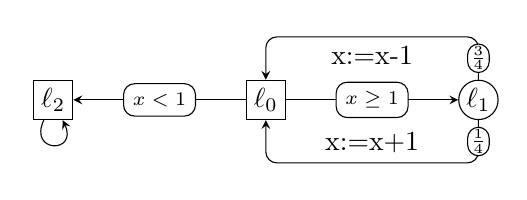
\begin{tikzpicture}[x = 1.8cm]
%\node[det] (det1) at (0,0) {$\loc_0$};
%\node[det] (while) at (1.5,-1.5)  {$\loc_1$};
%\node[det] (fin) at (0,-3) {$\loc_5$};
%\node[ran] (prob) at (3,-1.5) {$\loc_2$};
%\node[ang] (angel) at (3,0) {$\loc_3$};
%\node[dem] (demon) at (3,-3)  {$\loc_4$};
%
%\draw[tran] (det1) to node[auto, swap] {x:=0} (while);
%\draw[tran] (while) to node[font=\scriptsize,draw, fill=white, 
%rectangle,pos=0.3] {$x<0$} (fin);
%\draw[tran, loop, looseness = 5, in =-65, out = -115] (fin) to (fin);
%\draw[tran] (while) to node[font=\scriptsize,draw, fill=white, 
%rectangle,pos=0.3] {$x\geq 0$} (prob);
%\draw[tran] (prob) to node[font=\scriptsize,draw, fill=white, 
%rectangle,pos=0.3, inner sep = 1pt] {$\frac{6}{10}$} (angel);
%\draw[tran] (prob) to node[font=\scriptsize,draw, fill=white, 
%rectangle,pos=0.3, inner sep = 1pt] {$\frac{4}{10}$} (demon);
%\draw[tran] (demon) -- node[auto] {x:=x+1} (demon-|while) -- (while);
%\draw[tran] (angel) -- node[auto, swap] {x:=x+1} (angel-|while) -- (while);
%\draw[tran] (demon) to node[auto] {x:=x-1} (while);
%\draw[tran] (angel) to node[auto, swap] {x:=x-1} (while);

\node[det] (while) at (1.5,0)  {$\loc_0$};
%%\node[det] (fin) at (0,-3) {};
\node[ran] (prob) at (3,0) {$\loc_1$};
%\node[ang] (angel) at (3,0) {$\loc_3$};
%\node[dem] at (3,-3) (demon) {$\loc_4$};
%\node[det] (aif) at (2,-0.075) {$\loc_5$};
%\node[det] (aelse) at (3,-0.8) {$\loc_6$};
%\node[det] (dif) at (2,-3) {$\loc_7$};
%\node[det] (delse) at (3,-2.2) {$\loc_8$};
%\node[det] (det1) at (0,0) {$\loc_0$};
%\node[det] (while) at (1.5,-1.5)  {};
\node[det] (fin) at (0,0) {$\loc_2$};
%\node[ran] (prob) at (3,-1.5) {};
%\node[ang] (angel) at (3,0) {};
%\node[dem] at (3,-3) (demon) {};
%
%%\draw[tran] (det1) to node[auto, swap] {x:=0} (while);
\draw[tran] (while) to node[font=\scriptsize,draw, fill=white, 
rectangle,pos=0.5] {$x<1$} (fin);
\draw[tran, loop, looseness = 5, in =-65, out = -115] (fin) to (fin);
\draw[tran] (while) to node[font=\scriptsize,draw, fill=white, 
rectangle,pos=0.5] {$x\geq 1$} (prob);
%\draw[tran] (prob) to node[font=\scriptsize,draw, fill=white, 
%rectangle,pos=0.3, inner sep = 1pt] {$\frac{6}{10}$} (angel);
%\draw[tran] (prob) to node[font=\scriptsize,draw, fill=white, 
%rectangle,pos=0.3, inner sep = 1pt] {$\frac{4}{10}$} (demon);
%\draw[tran] (demon) -- node[auto] {x:=x+1} (demon-|while) -- (while);
%\draw[tran] (angel) -- node[auto, swap] {x:=x+1} (angel-|while) -- (while);
%\draw[tran] (demon) to node[auto] {x:=x-1} (while);
%\draw[tran] (angel) to node[auto, swap] {x:=x-1} (while);


%\draw[tran] (angel) -- (aif);
%\draw[tran] (angel) -- (aelse);
%\draw[tran] (demon) -- (dif);
%\draw[tran] (demon) -- (delse);

\node (dum1) at (0,0.8) {};
\node (dum2) at (0,-0.8) {};

\draw[tran] (prob) -- node[font=\scriptsize,draw, fill=white, 
rectangle,pos=0.5, inner sep = 1pt] {$\frac{3}{4}$} (prob|-dum1) -- node[auto] 
{x:=x-1}
(while|-dum1)--(while);
\draw[tran] (prob) -- node[font=\scriptsize,draw, fill=white, 
rectangle,pos=0.5, inner sep = 1pt] {$\frac{1}{4}$} (prob|-dum2) 
-- node[auto,swap] {x:=x+1} (while|-dum2)--(while);
%\draw[tran] (dif) --  (demon-|while) -- node[auto, pos=0.2] {x:=x+1} (while);
%\draw[tran] (aif) --  (angel-|while) -- node[auto, swap, pos=0.2] {x:=x+1} 
%(while);
%\draw[tran] (delse) -- node[auto] {x:=x-1} (delse-|while.305) --  (while.-55);
%\draw[tran] (aelse) -- node[auto, swap] {x:=x-1} (aelse-|while.55) --  
%(while.55);
\end{tikzpicture}
\caption{An \APP{} modelling an asymmetric 1-D random walk and the associated 
pCFG. Probabilistic locations are depicted by circles, with probabilities given 
on outgoing 
transitions. Transitions are labelled by their effects. Location $\loc_0$ is 
initial and $\loc_2$ is terminal.}
\label{fig:invariant-running}
\end{figure}


%%\vspace{-1em}
\section{Invariants and Ranking Supermartingales}\label{sec:invm}
%\vspace{-0.5em}

In this section we recall basic results on (one-dimensional) ranking 
supermartingales in probabilistic programs.

%In this section we recall known methods and constructs for solving the 
%qualitative termination and reachability questions for \APP{s}, namely  
%linear invariants and ranking supermartingales. 
%We also demonstrate that these methods are not sufficient to address the 
%quantitative variants of these questions (i.e., probabilistic termination).
%In order to discuss the necessary concepts, we recall the basics of 
%martingales, which is relevant for both this and subsequent sections. 
%Since the definitions of this section are from the literature we relegate
%relevant illustrations through example to the Appendix.

%While the core results of this section were already proven in the previous 
%literature, the version we sometimes present slight generalizations of these 
%result, which make them applicable to a larger class of programs. We discuss 
%the nature of these generalizations where appropriate.

%\vspace{-1em}
\subsection{Invariants}
%\vspace{-0.5em}

Invariants are a vital element of many program analysis techniques. 
Intuitively, invariants are maps assigning to each 
program location $\loc$ of some pCFG a predicate which is guaranteed to hold 
whenever $\loc$ is 
entered. 

\smallskip
\begin{definition}[Linear Predicate Maps (LPMs) and Invariants] We define the 
following:
\begin{compactenum}
\item
A \emph{linear predicate map (LPM)} for an \APP{} $P$ is a function $I$ 
assigning to each location $\loc$ of the pCFG $\pCFG_P$ a propositionally 
linear predicate $I(\loc)$ over the set of program variables of $P$.
\item
A \emph{linear invariant} (or just an invariant) for an \APP{} $P$ is 
a linear predicate map $\inv$ for $P$ with
the following property: for each location $\loc$ of $\pCFG_P$ and each finite 
path $(\loc_0,\vec{x}_0),\cdots,(\loc_n,\vec{x}_n)$ such that 
$(\loc_0,\vec{x}_0)=(\locinit,\vecinit)$ and $\loc_n = \loc$ it holds
$\vec{x}_n\models \inv(\loc)$.
\end{compactenum}
%%A 
%%probabilistic LPM for $P$ is a tuple $(\pinv,\pinfunc)$ such that $\pinv$ is 
%%a 
%%pure LPM for $P$ and $\pinfunc$ is a function assigning to each location 
%%$\loc$ 
%%a probability $\pi(\loc)\in[0,1]$.
\end{definition}



%A special class of LPMs are program invariants, i.e. maps assigning to each 
%program location $\loc$ an PLP which is guaranteed to hold whenever $\loc$ is 
%entered.
%Invariants are a standard construct used in automated program analysis. 
%To avoid confusion with probabilistic invariants, we call the 
%standard invariants \emph{pure}.
%
%\begin{definition}[Pure Linear Invariant]
%A \emph{pure linear invariant} (or just a pure invariant) for an \APP{} $P$ is 
%%a function map $\inv$  assigning to each location $\loc$ of the pCFG 
%%$\pCFG_P$ 
%%a propositionally 
%%linear predicate $I(\loc)$ over the set of program variables of $P$ 
%a linear predicate map $\inv$ for $P$ with
%the following property: for each location $\loc$ of $\pCFG_P$ and each finite 
%path $(\loc_0,\vec{x}_0),\cdots,(\loc_n,\vec{x}_n)$ such that 
%$(\loc_0,\vec{x}_0)=(\locinit,\vecinit)$ and $\loc_n = \loc$ it holds
%$\val_{\vec{x}_i}\models \inv(\loc)$.
%\end{definition}



%\vspace{-1em}
\subsection{Supermartingales}
%\vspace{-0.5em}

%Submartingales and their counterparts, supermartingales, are a standard tool 
%of 
(Super)martingales, are a standard tool of 
probability theory apt for analyzing probabilistic objects arising in computer 
science, from automata-based models~\cite{BKKNK:pMC-zero-reachability} to 
general probabilistic 
programs~\cite{SriramCAV,HolgerPOPL,CFNH16:prob-termination,CFG16:positivstellensatz-arxiv,BEFH16:doob-decomposition}.
 
%\PN{Maybe move this sentence to intro.} 
Let us first recall basic
definitions and results related to supermartingales, which we need in our 
analysis.

\smallskip\noindent{\bf Conditional Expectation.} 
%The notion of conditional expectation 
%tightly connected to martingales. We present only a brief informal exposition 
%here, for formal treatment see, e.g.~\cite[Chapter 9]{Williams:book}.
Let $(\Omega,\mathcal{F},\probm)$ be a probability space, 
$X\colon\Omega\rightarrow 
\Rset$ an $\mathcal{F}$-measurable function, and $\mathcal{F}'\subseteq 
\mathcal{F}$ sub-sigma-algebra of $\mathcal{F}$. The \emph{conditional 
expectation} of $X$ given $\mathcal{F}'$ is an $\mathcal{F}'$-measurable random 
variable denoted by $\E[X| \mathcal{F}']$ which satisfies, for each set $A\in 
\mathcal{F}'$, the following: 
\begin{equation}
\label{eq:cond-exp}
\E[X\cdot 1_A] = \E[\E[X|\mathcal{F}]\cdot 1_A],
\end{equation}
where $1_A \colon \Omega\rightarrow \{0,1\}$ is an \emph{indicator function} of 
$A$, i.e. function returning $1$ for 
each $\omega\in A$ and $0$ for each $\omega\in \Omega\setminus A$. Note that 
the left hand-side of~\eqref{eq:cond-exp} intuitively represents the expected 
value 
of $X(\omega)$ with domain restricted to $A$.

Recall that in context of probabilistic programs we work with probability 
spaces of the form $(\Omega,\natfilt,\probm^\sigma)$, where $\Omega$ is a 
set of runs in some $\pCFG$ and $\natfilt$ is (the smallest) sigma-algebra 
such that all the functions $\cfg{\sigma}{i}$, where $i\in \Nset_0$ and 
$\sigma$ is a scheduler, are $\natfilt$-measurable. In such a setting we can 
also consider sub-sigma-algebras $\natfilt_i$, $i\in \Nset_0$, of 
$\natfilt$, where $\natfilt_i$ is the smallest sub-sigma-algebra of 
$\natfilt$ such that all the functions $\cfg{\sigma}{j}$, $0\leq j \leq 
i$, are $\natfilt_i$-measurable. Intuitively, each set $A$ belonging to such 
an $\natfilt_i$ consists of runs whose first $i$ steps satisfy some 
property, and the probability space $(\Omega,\natfilt_i,\probm^\sigma)$ 
allows us to reason about probabilities of certain events happening in the 
first 
$i$ steps of program execution. 
%(note that since $\natfilt_i \subseteq 
%\natfilt$, we can view $\probm^\sigma$ also as a function of type 
%$\natfilt_i\rightarrow [0,1]$). 
Then, for each $A\in \natfilt_i$, the 
value $\E[\E[X|\natfilt_i]\cdot 1_A]$ represents the expected value of 
$X(\run)$ for the randomly generated run $\run$ provided that we restrict to 
runs whose
prefix of length $i$ satisfies the property given by $A$. 
Note that the sequence $\natfilt_0,\natfilt_1,\natfilt_2,\dots$ forms a 
filtration of $\natfilt$, which we call a \emph{canonical filtration}.

%%\paragraph*{Basics of Supermartingales}

\smallskip
\begin{definition}[Supermartingale]
Let $(\Omega,\mathcal{F},\probm)$ be a probability space and 
$\{\mathcal{F}_i\}_{i=0}^{\infty}$ a filtration of $\mathcal{F}$. A sequence of 
random variables $\{X_i\}_{i=0}^{\infty}$ is a \emph{supermartingale} w.r.t. 
filtration $\{\mathcal{F}_i\}_{i=0}^{\infty}$ if it satisfies these conditions:
\begin{compactenum}
\item  The process $\{X_i\}_{i=0}^{\infty}$ is \emph{adapted} to 
$\{\mathcal{F}_i\}_{i=0}^{\infty}$, i.e. for all $i\in \Nset_0$ it holds that 
$X_i$ is $\mathcal{F}_i$-measurable.
\item For all $i\in \Nset_0$ it holds $\E[|X_i|]<\infty$.
\item For all $i\in \Nset_0$ it holds 
\begin{equation}
\label{eq:supermart-def}
\E[X_{i+1}|\mathcal{F}_i] \leq X_i.
\end{equation}

A supermartingale $\{X_i\}_{i=0}^{\infty}$ has $c$-bounded differences, where 
$c\geq 0$, if $|X_{i+1}-X_i|<c$ for all $i\in \Nset_0$
\end{compactenum}
%A sequence of 
%random variables $\{X_i\}_{i=0}^{\infty}$ is a \emph{submartingale} w.r.t.  
%$\{\mathcal{F}_i\}_{i=0}^{\infty}$ if the process $\{-X_i\}_{i=0}^{\infty}$ is 
%a supermartingale w.r.t. the same filtration.
\end{definition}


Intuitively, a supermartingale is a stochastic process whose average value is 
guaranteed not to rise as time evolves, even if some information on the past 
evolution of the process is revealed. 
%Symmetrically, a submartingale is a 
%process whose value does not drop on average. 
We often need to work with supermartingales whose value 
is guaranteed to decrease on average, until a certain condition is 
satisfied. The point in time in which such a condition is satisfied is called a 
\emph{stopping time}.

\smallskip
\begin{definition}[Stopping time]
Let $(\Omega,\mathcal{F},\probm)$ be a probability space and 
$\{\mathcal{F}_i\}_{i=0}^{\infty}$ a filtration. A random variable $\stime 
\colon 
\Omega\rightarrow \Nset_0$ is called a \emph{stopping time} w.r.t. 
$\{\mathcal{F}_i\}_{i=0}^{\infty}$ if %$\stime$ is adapted to this filtration 
%and if 
for all $j\in \Nset_0$ the set $\{\omega\in \Omega\mid \stime(\omega)\leq j\}$ 
belongs to $\mathcal{F}_j$.
\end{definition}


In particular, for each set of configurations $C$ the reachability time 
$\treach{C}$ of $C$ is a stopping time w.r.t. the canonical filtration, since 
at each time $j$ we can decide whether $\treach{C}>j$ or not by looking at the 
prefix of a run of length $j$. 
%When $\Omega$ is a set of runs of some $\pCFG_P$, we can think of 
%$\stime$ as representing a 
%certain condition which can or cannot hold in a given time instance of the 
%execution of $P$, where $\stime(\run)$ represents the first point in time 
%during the execution represented by $\run$ in which $P$ holds. The condition 
%$\{\omega\in \Omega\mid \stime(\omega)\leq j\}\in \mathcal{F}_j$ then states 
%that whether $P$ holds at step $j$ of a run can be determined by looking at 
%the 
%prefix of the run of length $j$. In other words, the stopping condition cannot 
%``talk'' about future events. The typical stopping time we use in the context 
%of \APP{s} is the \emph{reachability} time $\treach{C}$ for some set of 
%configurations $C$, where $\treach{C}(\run)$ is the first point in time when 
%the current configuration on $\run$ is in $C$. In particular, if $C$ is the 
%set 
%of all configurations $(\loc,\vec{x})$ such that $\loc=\loc^\lout_P$ (the 
%terminal location of $\pCFG_P$), then we denote $\treach{C}$ by $\ttime$ and 
%call it a \emph{termination time} of $P$.
%We combine stopping conditions with martingales to get 
%\emph{$\eps$-decreasing} 
%supermartingales. %
Finally, we recall the fundamental notion of a ranking 
supermartingale.

\smallskip
\begin{definition}[Ranking supermartingale]
\label{def:ranking}
Let $(\Omega,\mathcal{F},\probm)$ be a probability space, 
$\{\mathcal{F}_i\}_{i=0}^{\infty}$ a filtration of $\mathcal{F}$, $\stime$ a 
stopping time w.r.t. that filtration, and $\eps\geq 
0$. 
A supermartingale $\{X_i\}_{i=0}^{\infty}$ (w.r.t. 
$\{\mathcal{F}_i\}_{i=0}^{\infty}$) is \emph{$\eps$-decreasing} until 
$\stime$ 
if it 
satisfies 
the following additional condition: for all $i\in \Nset_0$ it holds
\begin{equation}
\label{eq:ranking-sup}
\E[X_{i+1}|\mathcal{F}_i] \leq X_i - \eps\cdot\vec{1}_{\stime > i}.
\end{equation}

Further, $\{X_i\}_{i=0}^{\infty}$ is an \emph{$\eps$-ranking} supermartingale 
($\eps$-RSM) for $\stime$ if it 
is $\eps$-decreasing until $\stime$ and for 
each $\omega\in\Omega, j\in\Nset_0$ it holds $\stime(\omega)>j \Rightarrow 
X_j(\omega)\geq 0$.
%is a supermartingale w.r.t. $\{\mathcal{F}_i\}_{i=0}^{\infty}$. 
%A supermartingale $\{X_i\}_{i=0}^{\infty}$ is 
%is $\eps$-repulsing if for all $i\in \Nset_0$ it holds
%\begin{equation}
%\label{eq:repulsing-sub}
%\E[X_{i+1}|\mathcal{F}_i] \leq X_i - \eps\cdot\vec{1}_{\stime > i}.
%\end{equation}
\end{definition}
Intuitively, if $\stime$ is the reachability time $\treach{C}$ of some set $C$, 
then the previous definition requires that an $\eps$-ranking supermartingale 
must decrease by at least $\eps$ on average up to the point when $C$ is 
reached for a first time. After that, it must not increase (on average).
The above definition is a bit more general than the standard one in the
literature as we also consider reachability as opposed to only termination.


%Intuitively, until the condition specified by $\stime$ is satisfied, ranking 
%supermartingale is non-negative and at the same time decreasing by at least 
%$\eps$ on average, forming a probabilistic analogue of the classical ranking 
%functions. 

%We finish this part by noting that for some applications it is preferable to 
%work with supermartingales that have \emph{bounded differences.}

%\begin{definition}
%A supermartingale $\{X_i\}_{i=0}^{\infty}$ has $c$-bounded differences, where 
%$c\geq 0$, if $|X_{i+1}-X_i|<c$ for all $i\in \Nset_0$.
%\end{definition}
%Note that $\{X_i\}_{i=0}^{\infty}$ being an $\eps$-repulsing supermartingale 
%for 
%$\stime$ is 
%\emph{not} equivalent to $\{-X_i\}_{i=0}^{\infty}$ being an $\eps$-ranking 
%supermartingale for $\stime$.

%We typically work with $\eps$-ranking supermartingales whose initial value is 
%positive and $\eps$-repulsing supermartingales whose initial value is 
%negative. 
%Then, intuitively an $\eps$-ranking supermartingale is driven towards negative 
%values by at least $\eps$ in each step (on average) until it indeed becomes 
%negative, while an $\eps$-repulsing submartingale is driven \emph{away} from 
%positive values by at least $\eps$ per step, as long as it stays non-positive 
%(we cannot rule out that it eventually becomes positive, as the decrease by 
%$\eps$ is guaranteed only on average). 
%%Note that $\{X_i\}_{i=0}^{\infty}$ being an $\eps$-repulsing submartingale is 
%%\emph{not} equivalent to $\{-X_i\}_{i=0}^{\infty}$ being an $\eps$-ranking 
%%supermartingale.

\smallskip\noindent{\bf Martingales in Program Analysis.}
In the context of \APP{} analysis, we consider a special type of 
supermartingales given as functions of the current values of program variables. 
In this paper we focus on the case when these functions are \emph{linear}.

\smallskip
\begin{definition}[Linear Expression Map]
A \emph{linear expression map (LEM)} for an \APP{} $P$ is a function $\lem$ 
assigning to each program location $\loc$ of $\pCFG_P$ an affine expression 
$\lem(\ell)$ over the program variables of $P$.
\end{definition}

Each LEM $\lem$ and location $\loc$ determines an affine function $\lem(\loc)$ 
which takes as an argument an $n$-dimensional vector, where $n$ is the number 
of distinct variables in $P$. We use $\lem(\loc,\vec{x})$ as a shorthand 
notation for $\lem(\loc)(\vec{x})$. 
Martingales for \APP{} analysis are defined via a standard notion of 
pre-expectation~\cite{SriramCAV}. Intuitively, a pre-expectation of $\lem$ is a 
function which for each configuration $(\loc,\vec{x})$ returns the maximal
expected value of $\lem$ after one step is made from this configuration, where 
the maximum is taken over all possible non-deterministic choices.

\smallskip
\begin{definition}[Pre-Expectation]
Let $P$ be an \APP{} such that $\pCFG_P = 
(\locs,\pvars,\locinit,\vecinit,\transitions,\probdist,\guards)$ and let $\lem$ 
a 
linear expression map 
for~$P$. 
%Let $\locs$ 
%be the set of locations of $\pCFG_P$ and $\pvars$ its set of program 
%variables. 
The 
pre-expectation of $\lem$ is a function $\preexp{\lem}\colon \locs\times 
\Rset^{|\pvars|} \rightarrow \Rset$ defined as follows:
\begin{compactitem} %\itemsep1pt \parskip0pt \parsep0pt
\item 
if $\loc$ is a probabilistic location, then
$$\preexp{\lem}(\loc,\vec{x}):=\sum_{(\loc,1,\id_1,\loc')\in\transitions} 
Pr_{\loc}\left((\loc,1,\id_1,\loc')\right)\cdot
 \lem(\loc',\vec{x});$$
\item 
 if $\loc$ is a non-deterministic location, then
$$\preexp{\lem}(\loc,\vec{x}):=
\max_{(\loc,1,\id_1,\loc')\in\transitions}\lem(\loc',\vec{x});$$

%\item 
%$\mathrm{pre}_\eta(\loc,\mathbf{x}):=\min_{(\loc,id,\ell')\in\transitions}\eta\left(\loc',\mathbf{x}\right)$
% if $\loc$ is an angelic location;
\item 
if $\loc$ is a deterministic location, then for each $\vec{x}$ the value 
$\preexp{\lem}(\loc,\vec{x})$ is determined as follows: there is exactly one 
transition
$\tau=(\loc,j,\up,\loc')$ such that $\vec{x}\models G(\tau)$. We distinguish 
three cases:
\begin{compactitem}
\item If $\up\colon \Rset^{|\pvars|}\rightarrow \Rset$ is a function, then 
$$\preexp{\lem}(\loc,\vec{x}):= \lem(\loc',\vec{x}(j\leftarrow \up(\vec{x}))).$$
\item If $\up$ is a distribution $d$, then $$ \preexp{\lem}(\loc,\vec{x}):= 
\lem(\loc',\vec{x}(j\leftarrow \E[d])),$$ where $\E[d]$ is the expected value of the 
distribution $d$.
\item 
If $\up$ is a set, then $$ \preexp{\lem}(\loc,\vec{x}):= \max_{a\in\up}
\lem(\loc',\vec{x}(j \leftarrow a)).$$
\end{compactitem}
%$\mathrm{pre}_\eta(\loc,\mathbf{x}):=\eta(\loc',\expv_{\rvars}\left(f(\vec{x},\mathbf{r})\right))$
% if $\loc$ is a deterministic location, $(\loc,f,\loc')\in\transitions$ and 
%$\mathbf{x}\in G(\loc,f,\loc')$, where 
%$\expv_{\rvars}\left(f(\vec{x},\mathbf{r})\right)$ is the expected value of 
%$f(\vec{x},\cdot)$. %on $\rvars$ if $\vec{x}$ is treated as a constant vector.
\end{compactitem}
%\end{definition}
\end{definition}

\smallskip
\begin{definition}(Linear Ranking Supermartingale)
\label{def:lrsm}
Let $P$ be an \APP{} such that $\pCFG_P = 
(\locs,\pvars,\locinit,\vecinit,\transitions,\probdist,\guards)$, let $\inv$ be 
a linear predicate map and let 
$\confset\subseteq \locs \times \Rset^{|\pvars|}$ be some set of 
configurations. 
%\begin{compactenum}
%\item
A linear $\eps$-ranking supermartingale ($\eps$-LRSM) for $\confset$ 
supported by $\inv$ is a 
linear expression map $\lem$ for $P$ such that for all configurations 
$(\loc,\vec{x})$ of $\pCFG_P$ with
$(\loc,\vec{x})\not\in \confset$ and $\vec{x}\models \inv(\loc)$ the following 
two conditions hold:
\begin{compactitem}
%\item For all $(\loc,\vec{x})\in \locs\times\Rset^{|\pvars|}$ it holds
%\item For all  it holds 
\item
$\lem(\loc,\vec{x})\geq 0$
\item 
$\preexp{\lem}(\loc,\vec{x}) \leq \lem(\loc,\vec{x})-\eps$ 
\end{compactitem}
%\item
%\end{compactenum}
A linear $\eps$-ranking supermartingale supported by $\inv$ has 
$c$-bounded differences if for each $(\loc,\vec{x})$ such that $\vec{x}\models 
\inv(\loc)$ and each configuration $(\loc',\vec{x}')$ such that $(\loc,\vec{x}) 
(\loc',\vec{x}')$ is a path in $\pCFG_P$ it holds 
$|\lem(\loc,\vec{x})-\lem(\loc',\vec{x}')|\leq c$. 
\end{definition}


The relationship between $\eps$-LRSM in \APP{s}, (pure) invariants, and almost-sure termination 
is summarized in the following theorem. 
\smallskip
\begin{theorem}[{\cite[Theorem 1]{CFNH16:prob-termination}}]
\label{thm:old-ranking}
Let $P$ be an \APP{}, $\sigma$ a scheduler, and 
$(\Omega,\natfilt,\probm^\sigma)$ the corresponding probability space. Further, 
let $C$ be the set of terminating configurations of $\pCFG_P$ (i.e., the termination
location is reached), such that there exist an $\eps>0$ and an $\eps$-linear ranking 
supermartingale $\lem$ supported by a pure invariant $I$. 
%%for $\treach{C}$. 
Then 
\begin{compactenum}
\item
$\probm^{\sigma}(\ttime<\infty)=1$, i.e. termination is ensured almost-surely.
\item
$\E^{\sigma}[\ttime]<\lem(\locinit,\vecinit)/\eps$.
%\item
%If $\{X_i\}_{i=0}^{\infty}$  has $c$-bounded differences for some $c$, then 
%there exists a concentration bound $B$ for $\treach{C}$ such that $B\leq 
%({E^{\sigma}[X_0]}/{\eps})+1$.
\end{compactenum}
\end{theorem}


The previous result shows that if there exists  an $\eps$-LRSM 
supported by a pure invariant $I$, for $\eps>0$, then under each scheduler 
termination is ensured almost-surely.
We now demonstrate that pure invariants, though effective for almost-sure 
termination, are ineffective to answer probabilistic termination questions.


%\begin{figure}[t]
\lstset{language=affprob}
\lstset{tabsize=3}
\newsavebox{\nonterm}
\begin{lrbox}{\nonterm}
\begin{lstlisting}[mathescape]
$x:=30,y:=20$
while $y\geq 0$ do
	$x:=x+$sample$(\mathrm{Uniform}[-\frac{1}{4},1])$
	$y:=y+$sample$(\mathrm{Uniform}[-1,\frac{1}{4}])$
	while $x \leq 0$ do skip od
od
\end{lstlisting}
\end{lrbox}
\begin{figure}[t]
%%\centering
\usebox{\nonterm}
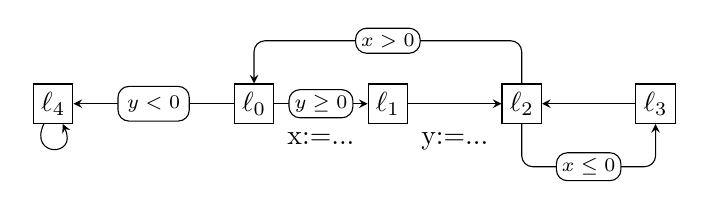
\begin{tikzpicture}[x = 1.7cm]
%\node[det] (det1) at (0,0) {$\loc_0$};
%\node[det] (while) at (1.5,-1.5)  {$\loc_1$};
%\node[det] (fin) at (0,-3) {$\loc_5$};
%\node[ran] (prob) at (3,-1.5) {$\loc_2$};
%\node[ang] (angel) at (3,0) {$\loc_3$};
%\node[dem] (demon) at (3,-3)  {$\loc_4$};
%
%\draw[tran] (det1) to node[auto, swap] {x:=0} (while);
%\draw[tran] (while) to node[font=\scriptsize,draw, fill=white, 
%rectangle,pos=0.3] {$x<0$} (fin);
%\draw[tran, loop, looseness = 5, in =-65, out = -115] (fin) to (fin);
%\draw[tran] (while) to node[font=\scriptsize,draw, fill=white, 
%rectangle,pos=0.3] {$x\geq 0$} (prob);
%\draw[tran] (prob) to node[font=\scriptsize,draw, fill=white, 
%rectangle,pos=0.3, inner sep = 1pt] {$\frac{6}{10}$} (angel);
%\draw[tran] (prob) to node[font=\scriptsize,draw, fill=white, 
%rectangle,pos=0.3, inner sep = 1pt] {$\frac{4}{10}$} (demon);
%\draw[tran] (demon) -- node[auto] {x:=x+1} (demon-|while) -- (while);
%\draw[tran] (angel) -- node[auto, swap] {x:=x+1} (angel-|while) -- (while);
%\draw[tran] (demon) to node[auto] {x:=x-1} (while);
%\draw[tran] (angel) to node[auto, swap] {x:=x-1} (while);

\node[det] (while) at (1.5,0)  {$\loc_0$};
%%\node[det] (fin) at (0,-3) {};
\node[det] (p1) at (2.5,0) {$\loc_1$};
\node[det] (p2) at (3.5,0) {$\loc_2$};

\node[det] (lp) at (4.5,0) {$\loc_3$};
%\node[ang] (angel) at (3,0) {$\loc_3$};
%\node[dem] at (3,-3) (demon) {$\loc_4$};
%\node[det] (aif) at (2,-0.075) {$\loc_5$};
%\node[det] (aelse) at (3,-0.8) {$\loc_6$};
%\node[det] (dif) at (2,-3) {$\loc_7$};
%\node[det] (delse) at (3,-2.2) {$\loc_8$};
%\node[det] (det1) at (0,0) {$\loc_0$};
%\node[det] (while) at (1.5,-1.5)  {};
\node[det] (fin) at (0,0) {$\loc_4$};
%\node[ran] (prob) at (3,-1.5) {};
%\node[ang] (angel) at (3,0) {};
%\node[dem] at (3,-3) (demon) {};
%
%%\draw[tran] (det1) to node[auto, swap] {x:=0} (while);
\node (dum1) at (0,0.8) {};
\node (dum2) at (0,-0.8) {};
\draw[tran] (while) to node[font=\scriptsize,draw, fill=white, 
rectangle,pos=0.5] {$y<0$} (fin);
\draw[tran, loop, looseness = 5, in =-65, out = -115] (fin) to (fin);
\draw[tran] (while) -- node[font=\scriptsize,draw, fill=white, 
rectangle,pos=0.5, inner sep = 2pt] {$y\geq0$} node[label={[label 
distance=0.12cm]-90:{x:=...}}] {} (p1);
\draw[tran] (p1) to node[label={[label 
distance=0.12cm]-90:{y:=...}}] {} (p2);
\draw[tran] (lp) to  (p2);
\draw[tran] (p2) -- (p2|-dum2) -- node[font=\scriptsize,draw, fill=white, 
rectangle,pos=0.5, inner sep = 2pt] {$x\leq 0$} (lp|-dum2) -- (lp);
\draw[tran] (p2) -- (p2|-dum1) -- node[font=\scriptsize,draw, fill=white, 
rectangle,pos=0.5, inner sep = 2pt] {$x> 0$} (while|-dum1) -- (while);
%\draw[tran] (prob) to node[font=\scriptsize,draw, fill=white, 
%rectangle,pos=0.3, inner sep = 1pt] {$\frac{4}{10}$} (demon);
%\draw[tran] (demon) -- node[auto] {x:=x+1} (demon-|while) -- (while);
%\draw[tran] (angel) -- node[auto, swap] {x:=x+1} (angel-|while) -- (while);
%\draw[tran] (demon) to node[auto] {x:=x-1} (while);
%\draw[tran] (angel) to node[auto, swap] {x:=x-1} (while);


%\draw[tran] (angel) -- (aif);
%\draw[tran] (angel) -- (aelse);
%\draw[tran] (demon) -- (dif);
%\draw[tran] (demon) -- (delse);



%\draw[tran] (prob) -- node[font=\scriptsize,draw, fill=white, 
%rectangle,pos=0.5, inner sep = 1pt] {$\frac{3}{4}$} (prob|-dum1) -- node[auto] 
%{x:=x-1}
%(while|-dum1)--(while);
%\draw[tran] (prob) -- node[font=\scriptsize,draw, fill=white, 
%rectangle,pos=0.5, inner sep = 1pt] {$\frac{1}{4}$} (prob|-dum2) 
%-- node[auto,swap] {x:=x+1} (while|-dum2)--(while);
%\draw[tran] (dif) --  (demon-|while) -- node[auto, pos=0.2] {x:=x+1} (while);
%\draw[tran] (aif) --  (angel-|while) -- node[auto, swap, pos=0.2] {x:=x+1} 
%(while);
%\draw[tran] (delse) -- node[auto] {x:=x-1} (delse-|while.305) --  (while.-55);
%\draw[tran] (aelse) -- node[auto, swap] {x:=x-1} (aelse-|while.55) --  
%(while.55);
\end{tikzpicture}
\caption{A program with infinitely many reachable configurations which 
terminates with high probability, but not almost 
surely, together with a sketch of its pCFG. }\label{fig:nonterm}
\end{figure}

%We now show why this approach does not work for the probabilistic reachability and termination. 

\smallskip
\begin{example}\label{ex:nonterm}
Consider the program in Figure~\ref{fig:nonterm}. 
In each 
iteration of the outer loop each of the variables is randomly modified by 
adding a number drawn from some uniform distribution.
%incremented or 
%decremented. The probability of incrementing $x$ is $\frac{3}{8}$, for
%decrementing $x$ it is $\frac{1}{8}$; the probability of incrementing $y$ it 
%is 
%$\frac{1}{8}$ and for decrementing $y$ it is $\frac{3}{8}$. 
Average increase of $x$ in each iteration is $\frac{3}{8}$, while average decrease 
of $y$ is $-\frac{3}{8}$.  It is easy to see that a program does not 
terminate almost-surely: 
there is for instance a tiny but non-zero probability of $x$ being decremented 
by at least $\frac{1}{8}$ in 
each of the first 240 loop iterations, after which we are stuck in the infinite 
inner 
loop. On 
the other hand, the expectations above show that there is a ``trend'' of $y$ 
decreasing and $x$ increasing, and executions that follow this trend eventually 
decrement $y$ below $0$ without entering the inner loop. Hence, the 
probabilistic intuition tells us that the program terminates with a high 
probability. However, the techniques of this section cannot prove 
this high-probability termination, since existence of an $\eps$-LRSM (with 
$\eps>0$) supported by a pure invariant already implies a.s. termination,
and so no such $\eps$-LRSM can exist for the program. 
\end{example}

In the next section we generalize the notion of pure invariants to stochastic invariants
for probabilistic termination to resolve issues like Example~\ref{ex:nonterm}.

%Adirect consequence of Theorems~\ref{thm:pure-supermart} is the following 
%connection 
%between pure invariants, 
%linear ranking supermartingales, and reachability properties. 
%
%\begin{corollary}
%\label{col:linear-ranking-old}
%Let $\lem$ be a linear $\eps$-ranking supermartingale for some set $C$ of 
%configurations of an \APP{} $P$ such that $\lem$ is supported by some pure 
%invariant of $P$. Then under every scheduler $\sigma$ it holds:
%
%\begin{compactenum}
%\item
%$\probm^{\sigma}(\treach{C}<\infty)=1$, i.e. the set $C$ is reached 
%almost-surely
%\item
%$\E^{\sigma}[\treach{C}]<\lem(\locinit,\vecinit)/\eps$.
%\item
%If $\{\lem(\cfg{\sigma}{i})\}_{i=0}^{\infty}$  has $c$-bounded differences for 
%some $c$, then 
%there exists a concentration bound $B$ for $\treach{C}$ such that $B\leq 
%({\lem(\locinit,\vecinit)}/{\eps})+1$.
%\end{compactenum}
%\end{corollary}







%\begin{proof}
%Denote $X_i = \lem(\cfg{\sigma}{i})$. To prove that 
%\end{proof}

%\begin{example}
%If we apply Theorem~\ref{thm:pure-supermart} on the $\frac{1}{4}$-LRSM $\lem$ 
%in Example~\ref{ex:lrsm}, we get exactly the process $\{X'_i\}_{i=0}^{\infty}$ 
%described in Example~\ref{ex:rsm}.
%\end{example}

%Having a supermartingale which decreases, on average, by some constant until 
%$C$ is reached effectively proves that $C$ is reached almost surely, very much like 
%the standard ranking functions prove that non-probabilistic program terminates. 
%Moreover, we can use such a supermartingale to prove additional assertions 
%about the reachability time.

%\begin{theorem}[variant of {\cite[Theorem 1]{CFNH16:prob-termination}}]
%\label{thm:old-ranking}
%Let $P$ be an \APP{}, $\sigma$ a scheduler, and 
%$(\Omega,\natfilt,\probm^\sigma)$ the corresponding probability space. Further, 
%let $C$ be a set of 
%configurations of $\pCFG_P$ such 
%that there exist an $\eps>0$ and an $\eps$-ranking supermartingale  
%$\{X_i\}_{i=0}^{\infty}$
%for $\treach{C}$. Then 
%\begin{compactenum}
%\item
%$\probm^{\sigma}(\treach{C}<\infty)=1$, i.e. the set $C$ is reached 
%almost-surely
%\item
%$\E^{\sigma}[\treach{C}]<\E^{\sigma}[X_0]/\eps$.
%\item
%If $\{X_i\}_{i=0}^{\infty}$  has $c$-bounded differences for some $c$, then 
%there exists a concentration bound $B$ for $\treach{C}$ such that $B\leq 
%({E^{\sigma}[X_0]}/{\eps})+1$.
%\end{compactenum}
%\end{theorem}

%\begin{remark}
%We again somewhat generalize the results of~\cite{CFNH16:prob-termination}, 
%where the 
%supermartingale 
%$\{X_i\}_{i=0}^{\infty}$ was additionally required to satisfy the 
%following: there exists $K>0$ such that with probability $1$ it holds $X_i > 
%-K$ for all $i$. We avoid this requirement by use of \emph{stopped ranking 
%supermartingale property} similar to~\cite[Section 10.9]{Williams:book}.
%\end{remark}





%Note that the requirement~\eqref{eq:ranking-sup} can be equivalently expressed 
%by stipulating that $\E[X_{i+1}|\mathcal{F}_i] \leq X_i - \eps\cdot 
%\vec{1}_{\{X_i \geq 0\}}$






\section{Lexicographic Supermartingales}
\label{sec:lexicographic}

In this section we introduce the notion of a \emph{lexicographic ranking 
supermartingale}, which generalizes the standard notion of ranking 
supermartingales. However, to define any form of a supermartingale, we need the crucial notion of conditional expectation.

\smallskip\noindent{\bf Conditional Expectation.} 
%The notion of conditional expectation 
%tightly connected to martingales. We present only a brief informal exposition 
%here, for formal treatment see, e.g.~\cite[Chapter 9]{Williams:book}.
Let $(\Omega,\mathcal{F},\probm)$ be a probability space, 
$X\colon\Omega\rightarrow 
\Rset$ an $\mathcal{F}$-measurable function, and $\mathcal{F}'\subseteq 
\mathcal{F}$ sub-sigma-algebra of $\mathcal{F}$. A \emph{conditional 
	expectation} of $X$ given $\mathcal{F}'$ is an $\mathcal{F}'$-measurable random 
variable denoted by $\E[X| \mathcal{F}']$ which satisfies, for each set $A\in 
\mathcal{F}'$, the following: 
\begin{equation}
\label{eq:cond-exp}
\E[X\cdot 1_A] = \E[\E[X|\mathcal{F}]\cdot 1_A],
\end{equation}
where $1_A \colon \Omega\rightarrow \{0,1\}$ is an \emph{indicator function} of 
$A$, i.e. function returning $1$ for 
each $\omega\in A$ and $0$ for each $\omega\in \Omega\setminus A$. Note that 
the left hand-side of~\eqref{eq:cond-exp} intuitively represents the expected 
value 
of $X(\omega)$ with domain restricted to $A$.

Note that any $\mathcal{F}'$-measurable random variable satisfying~\eqref{eq:cond-exp} can be called a conditional expectation. The definition does not guarantee that the conditional expectation is uniquely defined or that it exists at all. However, from probability theory we have the following:

\begin{proposition}
\label{prop:conditional-exp-existence}
Let $(\Omega,\mathcal{F},\probm)$ be a probability space, 
$X\colon\Omega\rightarrow 
\Rset$ an $\mathcal{F}$-measurable function, and $\mathcal{F}'\subseteq 
\mathcal{F}$ sub-sigma-algebra of $\mathcal{F}$. Assume that one of the following conditions hold:
\begin{itemize}
\item $\E[|X|]<\infty$; or
\item $X$ is non-negative and for all $\omega\in\Omega$ it holds $X(\omega)\neq \infty$.
\end{itemize}
Then there exists a conditional expectation of $X$ given $\mathcal{F}'$ and it is almost-surely unique, i.e. for each two $\mathcal{F}'$-measurable functions $f$, $g$ that satisfy~\eqref{eq:cond-exp} it holds $\probm(\{\omega\mid f(\omega)\neq g(\omega)\})=0$.
\end{proposition}
\begin{proof}
The proof for the case when $\E[|X|]$ is standard and appears in many textbooks on probability theory (e.g.~\cite{Billingsley:book,Ash:book,Rosenthal:book}). The proof for the second case is essentially the same: the condition that $X$ is non-negative and not admitting infinite value suffices for satisfying the assumptions of Radon-Nikodym Theorem, the main theoretical tool used in the proof. For the sake of completeness we present the proof in \AppendixMaterial.
\end{proof}

Since the constraint~\eqref{eq:cond-exp} defining conditional expectation is phrased in terms of expected values, the almost-sure uniqueness cannot be strengthened to uniqueness, as re-defining a random variable on a set of probability zero does not change its expectation. In the following, when we say that a conditional expectation of a random variable $X$ satisfies some inequality (e.g. $\E[X\mid\mathcal{F}]\geq 0$) on set $L\subseteq \Omega$, we mean that for each $\mathcal{F}$-measurable function $\E[X\mid\mathcal{F}]$ satisfying~\eqref{eq:cond-exp} the .

In context of probabilistic programs we work with probability 
spaces of the form $(\Omega,\natfilt,\probm^\sigma)$, where $\Omega$ is a 
set of runs in some $\pCFG$ and $\natfilt$ is (the smallest) sigma-algebra 
such that all the functions $\cfg{\sigma}{i}$, where $i\in \Nset_0$ and 
$\sigma$ is a scheduler, are $\natfilt$-measurable. In such a setting we can 
also consider sub-sigma-algebras $\natfilt_i$, $i\in \Nset_0$, of 
$\natfilt$, where $\natfilt_i$ is the smallest sub-sigma-algebra of 
$\natfilt$ such that all the functions $\cfg{\sigma}{j}$, $0\leq j \leq 
i$, are $\natfilt_i$-measurable. Intuitively, each set $A$ belonging to such 
an $\natfilt_i$ consists of runs whose first $i$ steps satisfy some 
property, and the probability space $(\Omega,\natfilt_i,\probm^\sigma)$ 
allows us to reason about probabilities of certain events happening in the 
first 
$i$ steps of program execution. 
%(note that since $\natfilt_i \subseteq 
%\natfilt$, we can view $\probm^\sigma$ also as a function of type 
%$\natfilt_i\rightarrow [0,1]$). 
Then, for each $A\in \natfilt_i$, the 
value $\E[\E[X|\natfilt_i]\cdot 1_A]$ represents the expected value of 
$X(\run)$ for the randomly generated run $\run$ provided that we restrict to 
runs whose
prefix of length $i$ satisfies the property given by $A$. 
The sequence $\natfilt_0,\natfilt_1,\natfilt_2,\dots$ forms a 
filtration of $\natfilt$, which we call a \emph{canonical filtration}.

\begin{definition}
Let $(\Omega,\genfilt,\probm)$ be a probability space and $O\subseteq \Omega$ some set.
 We say that sets $L_1,\dots,L_n$ form an almost-sure partition of $O$ if $L_1,\dots,L_n$ are pairwise disjoint and $\probm(\{\omega\in O\mid \omega \not \in L_1\cup\dots \cup L_n\})=0$
\end{definition}

\begin{definition}[Lexicographic Ranking Supermartingale]
Let $(\Omega,\genfilt,\probm)$ be a probability space, 
$\{\genfilt_i\}_{i=0}^{\infty}$ a filtration of $\genfilt$, $\stime$ a stopping 
time w.r.t. that filtration, and 
$\eps\geq 0$. 
An $n$-dimensional stochastic process $\{\vec{X}_{i}\}_{i=0}^{\infty}$ is a 
\emph{lexicographic $\eps$-ranking supermartingale for $\stime$ 
($\eps$-LexRSM)} if the 
following 
conditions hold:
\begin{compactenum}
\item For each $1\leq j \leq n$ the 1-dimensional stochastic process 
$\{\vecseq{X}{i}{j}\}_{i=0}^{\infty}$ is adapted to 
$\{\genfilt_i\}_{i=0}^{\infty}$.
%\item For each $i\in \Nset_0$ and each $1\leq j \leq n$ it holds 
%$\E[|\vecseq{X}{i}{j}|]<\infty$.
\item For each $\omega \in \Omega$, $i\in \Nset_0$ and $1\leq j \leq n$ it holds 
$\vec{X}_i (\omega)[j]\geq {0}$ and $\vec{X}_i(\omega)[j]\neq \infty$.
\item For each $i\in \Nset_0$ there exists an almost-sure partition of the set $\{\stime>i\}$ into $n$ subsets $L^i_1,\dots,L^i_n$, all of them $\genfilt_i$-measurable, such that for each $1\leq j \leq n$:
\begin{compactitem}
	\item $\E[\vecseq{X}{i+1}{j}\mid 
	\genfilt_i]\leq\vecseq{X}{i}{j} - 
	\eps$ on $L_j$; and
	\item for all $1 \leq j' < j$ we have $\E[\vecseq{X}{i+1}{j'}\mid 
	\genfilt_i]=\vecseq{X}{i}{j'}$ on $L_{j}$.
\end{compactitem}
\end{compactenum}
\end{definition}

The 1-dimensional lexicographic $\eps$-ranking supermartingale is, to a large extent, equivalent to the notion of a ranking supermartingale as studied in~\cite{xxx}. There is one significant difference: in~\cite{xxx} there is an additional \emph{integrability} condition imposed on the one-dimensional process $\{X_i\}_{i=0}^{\infty}$, which requires that for each $i\geq 0$ it holds $\E[|X_i|]<\infty$ (or equivalently $\E[X_i]<\infty$, as the process is required to be non-negative). We do not impose this condition, and indeed, it is possible to define a 3-dimensional LexRSM $\{\vec{X}_{i}\}_{i=0}^{\infty}$ such that $\E[X[3]_i]=\infty$ for some $i$ \textbf{[PETR: EXAMPLE]}. However, closer inspection of proofs in~\cite{xxx} that link 1-dimensional ranking supermartingales to a.s. termination reveals that the integrability condition is never explicitly used there. Indeed, the only point in which integrability is needed is to ensure that the conditional expectations exist and are well-defined. However, the existence of conditional expectations is also guaranteed for random variables that are non-negative, even if their expected value if infinite, see Theorem~\ref{xxx}. This is exactly the case in both the original 1-dimensional ranking supermartingales and our generalization to LexRSMs. Below we show, that also in the LexRSM case we do not need integrability to prove a.s. termination, and hence we drop the condition altogether. This is particularly relevant when applying LexRSMs to programs with non-linear arithmetic, where proving integrability of LexRSM is more difficult than in the affine case, see Example~\ref{xxx}. 

\begin{theorem}
Let $(\Omega,\genfilt,\probm)$ be a probability space, 
$\{\genfilt_i\}_{i=0}^{\infty}$ a filtration of $\genfilt$, and $\stime$ a 
stopping 
time w.r.t. that filtration. If there exists an $\eps$-LexRSM for $\stime$, 
then $\probm(\stime<\infty)=1$.
\end{theorem}
\begin{proof}
The proof proceeds by contradiction, i.e. we assume that an $\eps$-LexRSM for 
$\stime$ exists and $\probm(\stime=\infty)>0$. For succinctness we denote the 
set $\{\omega\mid \stime(\omega)=\infty\}$ by $\genRunSet_{\infty}$.

For $\omega\in \Omega$ we define the level of $\omega$ at step $i$ to be the 
number $\levelrank{\omega}{i}$ equal to either $0$, if $\stime(\omega)\leq i$ or $\omega$ does not belong to $L^i_1 \cup \dots\cup L^i_n$, 
or otherwise to the $1\leq j \leq n$ such that $\omega\in L^i_j$. By the definition of 
$\eps$-LexRSM the value $\levelrank{\omega}{i}$ is well-defined for all 
$\omega$ and moreover, the random variable $\levelrank{}{i}$ is $\genfilt_i$-measurable. We denote by $\minlev(\omega)$ the smallest $0 \leq j \leq n$ such 
that $j$ is a level of $\omega$ at infinitely many steps. Note that $\omega \in 
\genRunSet_{\infty}$ implies $\minlev(\omega)\neq 0$, and $\probm(\genRunSet_{\infty})=\probm(\{\minlev \neq 0 \})$, as for each $i$ almost all $\omega$'s for which $\stime(\omega)>i$ belong to $L^i_1 \cup \dots\cup L^i_n$. We denote by $M_i$ 
the set of all $\omega$'s with $\minlev(\omega)=i$.

Throughout the proof we use several times the following fundamental fact: if 
$\probm(A)>0$ for some set $A$ and $A=A_1\cup A_2 \cup A_3\cdots$ for some 
sequence of sets $A_1,A_2,A_3,\dots$, then there exists $i$ such that 
$\probm(A_i)>0$.

Now since $\genRunSet_{\infty}=M_1,\dots,M_n$, there must be $1\leq \fixn{j} \leq n$ 
s.t. $\probm(M_{\fixn{j}})>0$. For each $\omega\in M_{\fixn{j}}$ there is the smallest number
${i}_{\omega,\fixn{j}}\in\Nset_0$ such that for all $i\geq {i}_{\omega,{j}}$ it holds 
$\levelrank{\omega}{i}\geq \fixn{j}$. Denote by $S_{\fixn{j},{i}}$ the set of all $\omega$'s in $M_{\fixn{j}}$ s.t. 
$i_{\omega,\fixn{j}}={i}$. 
Since $M_{\fixn{j}} = M_{\fixn{j},1} \cup M_{\fixn{j},2} \cup M_{\fixn{j},3} \cup \cdots$, there is $\fixn{i}\in 
\Nset_0$ 
s.t. 
$\probm(M_{\fixn{j},\fixn{i}})>0$. Continuing on the same note, for each $B\in \Nset$ we 
denote by $M_{\fixn{j},\fixn{i}}^{B}$ the set off all $\omega$'s in $M_{\fixn{j},\fixn{i}}$ s.t. 
$\vecseq{X}{\fixn{i}}{\fixn{j}}(\omega)\leq B$. Since $M_{\fixn{j},\fixn{i}}= M_{\fixn{j},\fixn{i}}^{1} \cup M_{\fixn{j},\fixn{i}}^{2} 
\cup M_{\fixn{j},\fixn{i}}^{3} \cup \cdots  $, there is $\fixn{B}\in \Nset$ s.t. 
$\probm(M_{\fixn{j},\fixn{i}}^{\fixn{B}})>0$. Denote $\fixn{p}=\probm(M_{\fixn{j},\fixn{i}}^{\fixn{B}})$.

Let $D$ be the set of all $\omega\in \Omega$ such that 
$\vecseq{X}{\fixn{i}}{\fixn{j}}(\omega)\leq \fixn{B}$. Note that $M_{\fixn{j},\fixn{i}}^{B} \subseteq D$ and $D\in 
\genfilt_i$ (and thus also $D\in \genfilt_{i'}$ for all $i'\geq i$). 
Define a stopping time $U$ w.r.t. filtration $\{\genfilt_i\}_{i=0}^{\infty}$ as follows: for all $\omega \in \Omega$ 
we put 
$U(\omega)=\inf\{k\in \Nset_0 \mid k\geq \fixn{i} \text{ and }
\levelrank{\omega}{k} < \fixn{j} \}$.

Define a 
(one-dimensional) stochastic process $\{Y_k\}_{k=0}^{\infty}$ as 
follows:
$$
Y_k(\omega) = \begin{dcases}
0 & \text{if $\omega \not\in D$}\\
\fixn{B} & \text{if $\omega \in D$ and $k<\fixn{i}$ }\\
\vecseq{X}{k}{\fixn{j}}(\omega) & \text{if $\omega \in D$, $k\geq \fixn{i}$ and 
$U(\omega)>k$ 
}\\
\vecseq{X}{U(\omega)}{\fixn{j}}(\omega) & \text{if $\omega\in D$, $k\geq 
\fixn{i}$ and 
$U(\omega)\leq k$ }.
\end{dcases}
$$

We prove several properties of the process $\{Y_k\}_{k=0}^{\infty}$. 
First, clearly for all $k\geq 0$, $Y_k(\omega)\geq 0$. Second, for each $k\geq \fixn{i}$, the variable $Y_k$ is $\genfilt_k$-measurable, as $D\in \genfilt_{\fixn{i}}$, $\{\vecseq{X}{i}{\fixn{j}}(\omega)\}_{i=0}^{\infty}$ is adapted to the filtration $\{\genfilt_i\}_{i=0}^{\infty}$ and $U$ is a stopping time w.r.t. this filtration. Finally, for any $k\in \Nset_0$ denote by 
$\noofdec_k$ the random variable such that $\noofdec_k(\omega) = |\{i'\in 
\Nset\mid \fixn{i} \leq i' < k \text{ and } \levelrank{\omega}{i'}=\fixn{j}\} |$.
We claim 
that for each $k\geq \fixn{i}$ 
it holds 
\begin{equation}
\label{eq:lexrsm-soundness-main}
\E[Y_k]\leq \fixn{B}\cdot \probm(D) - \eps\cdot\sum_{\ell=0}^{k-\fixn{i}} \ell\cdot\probm(D 
\cap \{U\geq k\} \cap \{\noofdec_k 
= 
\ell\}).
\end{equation}

The proof of~\eqref{eq:lexrsm-soundness-main} goes by induction on $k$. For 
$k=\fixn{i}$ the sum on the right-hand side equals $0$, so the 
inequality immediately follows from the definition of $Y_k$. Now assume 
that~\eqref{eq:lexrsm-soundness-main} holds for some $k\geq \fixn{i}$. We have that 
\begin{align}
\label{eq:lexrsm-ind-1}
\E[Y_{k+1}] &= \underbrace{\E[Y_{k+1}\cdot \indicator{\Omega\setminus D}]}_{=0=\E[Y_k\cdot\indicator{\Omega\setminus D}]} +  \underbrace{\E[Y_{k+1}\cdot \indicator{D \cap \{U \leq k\}}]}_{=\E[Y_k\cdot\indicator{D\cap \{U\leq k\}}]} + \underbrace{\E[Y_{k+1}\cdot \indicator{D \cap \{U > k\}}]}_{=\E[\vecseq{X}{k+1}{\fixn{j}}\cdot\indicator{D\cap \{U>k \} }]},
\end{align}
where the equality $\E[Y_{k+1}\cdot \indicator{D \cap \{U \leq k\}}] =\E[Y_k\cdot\indicator{D\cap \{U\leq k\}}] $ follows from the fact that $Y_{k+1}(\omega)=Y_k({\omega})=\vecseq{X}{U(\omega)}{\fixn{j}}(\omega)$ for $\omega\in \{U\leq k\}$, and similarly for the last term. We prove that 
\begin{equation}
\label{eq:lexrsm-ind-2}
\E[\vecseq{X}{k+1}{\fixn{j}}\cdot \indicator{D\cap \{U > k \}}] \leq \E[Y_k\cdot \indicator{D\cap \{U > k \}} -\eps\cdot \indicator{D\cap \{U>k\} \cap \{\levelrank{}{k}= \fixn{j}\} }] .
\end{equation}
Indeed, it holds
\begin{equation}
\label{eq:lexrsm-ind-3}
\E[\vecseq{X}{k+1}{\fixn{j}}\cdot \indicator{D\cap \{U > k \}}] = \E[\vecseq{X}{k+1}{\fixn{j}}\cdot \indicator{D\cap \{U > k \} \cap \{\levelrank{}{k}=\fixn{j} \} }]  + \E[\vecseq{X}{k+1}{\fixn{j}}\cdot \indicator{D\cap \{U > k \} \cap \{\levelrank{}{k}>\fixn{j}\} }], 
\end{equation}
since $\levelrank{\omega}{k}\geq \fixn{j}$ for all $\omega \in \{U>k\}$. Since the set $D\cap \{U > k \} \cap \{\levelrank{}{k}=\fixn{j} \}$ is $\genfilt_k$-measurable, we get
\begin{align}
\E[\vecseq{X}{k+1}{\fixn{j}}\cdot \indicator{D\cap \{U > k \} \cap \{\levelrank{}{k}=\fixn{j} \} }] &= \E[\E[\vecseq{X}{k+1}{\fixn{j}}\mid \genfilt_k]\cdot \indicator{D\cap \{U > k \} \cap \{\levelrank{}{k}=\fixn{j} \} }] \label{eq:lexrsm-ind-4}\\
&\leq \E[(\vecseq{X}{k}{\fixn{j}} - \eps)\cdot \indicator{D\cap \{U > k \} \cap \{\levelrank{}{k}=\fixn{j} \}}] \label{eq:lexrsm-ind-5}\\
&=\E[(Y_k - \eps)\cdot \indicator{D\cap \{U > k \} \cap \{\levelrank{}{k}=\fixn{j} \}}] \label{eq:lexrsm-ind-6},
\end{align}
where~\eqref{eq:lexrsm-ind-4} follows from the definition of conditional expectation~\eqref{eq:cond-exp},~\eqref{eq:lexrsm-ind-5} follows from the definition of $\{\levelrank{}{k}=\fixn{j}\}$, and~\eqref{eq:lexrsm-ind-6} holds since $Y_k(\omega)=\vecseq{X}{k}{\fixn{j}}(\omega)$ for $\omega$ with $U(\omega)> k$. Almost identical argument shows that
\begin{equation}
\label{eq:lexrsm-ind-7}
\E[\vecseq{X}{k+1}{\fixn{j}}\cdot \indicator{D\cap \{U > k \} \cap \{\levelrank{}{k}>\fixn{j} \} }] \leq \E[Y_k\cdot \indicator{D\cap \{U > k \} \cap \{\levelrank{}{k}>\fixn{j} \}}].
\end{equation}
Plugging~\eqref{eq:lexrsm-ind-6} and~\eqref{eq:lexrsm-ind-7} into~\eqref{eq:lexrsm-ind-3} yields~\eqref{eq:lexrsm-ind-2}. Now we can plug~\eqref{eq:lexrsm-ind-2} into~\eqref{eq:lexrsm-ind-1} to get
\begin{align}
\E[Y_{k+1}]&\leq \E[Y_k] - \eps\cdot \E[\indicator{D \cap \{U>k\} \cap \{\levelrank{}{k} = \fixn{j} \} }] = \E[Y_k] - \eps\cdot \probm(D \cap \{U>k\} \cap \{\levelrank{}{k} = \fixn{j} \} ) \nonumber\\
&\leq \fixn{B}\cdot \probm(D) - \eps\cdot\left(\sum_{\ell=0}^{k-\fixn{i}} \ell\cdot\probm(D 
\cap \{U\geq k\} \cap \{\noofdec_k = \ell\})\right) -\eps\cdot \probm(D \cap \{U>k\} \cap \{\levelrank{}{k} = \fixn{j} \}),
\end{align}
where the last inequality follows from induction hypothesis. Hence, using $D_{k,\ell}$ as a shorthand for $D 
\cap \{U\geq k\} \cap \{\noofdec_k = \ell\}$, to prove~\eqref{eq:lexrsm-soundness-main} it remains to show that
\begin{equation}
\label{eq:lexrsm-ind-8}
\sum_{\ell=0}^{k-\fixn{i}} \ell\cdot\probm(D_{k,\ell}) + \probm(D \cap \{U>k\} \cap \{\levelrank{}{k} = \fixn{j} \}) = \sum_{\ell=0}^{k+1-\fixn{i}} \ell\cdot\probm(D_{k+1,\ell}).
\end{equation}
The left-hand side of~\eqref{eq:lexrsm-ind-8} is equal to
\begin{align}
&\phantom{+}\;\sum_{\ell=0}^{k-\fixn{i}} \ell\cdot\probm(D_{k,\ell} \cap \{\levelrank{}{k}=\fixn{j}\}) + \sum_{\ell=0}^{k-\fixn{i}} \ell\cdot\probm(D_{k,\ell}\cap \{\levelrank{}{k}>\fixn{j}\} )\nonumber \\ 
&+\sum_{\ell=0}^{k-\fixn{i}}\probm(\underbrace{D \cap \{U>k\} \cap \{\levelrank{}{k} = \fixn{j}\} \cap \{\noofdec_k = \ell\}}_{=D_{k,\ell} \cap \{\levelrank{}{k} = \fixn{j}\}})
\nonumber \\
&= \sum_{\ell=0}^{k-\fixn{i}}(\ell+1) \cdot\probm(D_{k,\ell}\cap \{\levelrank{}{k} = \fixn{j}\}) +  \sum_{\ell=0}^{k-\fixn{i}} \ell\cdot\probm(D_{k,\ell}\cap \{\levelrank{}{k}>\fixn{j}\} ) \nonumber\\
&=\sum_{\ell=0}^{k-\fixn{i}} (\ell+1)\cdot \probm{(D_{k+1,\ell+1} \cap \{\levelrank{}{k} = \fixn{j}\})} +  \sum_{\ell=0}^{k-\fixn{i}} \ell\cdot\probm(D_{k+1,\ell}\cap \{\levelrank{}{k}>\fixn{j}\} ) \label{eq:lexrsm-ind-9}\\
&= \sum_{\ell=1}^{k+1-\fixn{i}} \ell\cdot \probm{(D_{k+1,\ell} \cap \{\levelrank{}{k} = \fixn{j}\})} +  \sum_{\ell=0}^{k-\fixn{i}} \ell\cdot\probm(D_{k+1,\ell}\cap \{\levelrank{}{k}>\fixn{j}\} )
   \nonumber \\
&= (k+1-\fixn{i})\cdot \probm{(D_{k+1,k+1-\fixn{i}}\cap\{\levelrank{}{k} =\fixn{j} \} )} + \sum_{\ell=1}^{k-\fixn{i}} \ell \cdot \probm(D_{k+1,\ell})  \nonumber\\
&= (k+1-\fixn{i})\cdot\probm(D_{k+1,k+1-\fixn{i}}) + \sum_{\ell=1}^{k-\fixn{i}}\ell\cdot\probm(D_{k+1,\ell}) = \text{ right-hand side of~\eqref{eq:lexrsm-ind-8}} \label{eq:lexrsm-ind-11}.
\end{align}
The individual steps in the above computation are justified as follows: in~\eqref{eq:lexrsm-ind-9} we use the facts that for all $\omega$'s whose level in step $k$ is $\fixn{j}$ it holds that $\noofdec_k(\omega)+1=\noofdec_{k+1}(\omega)$, and similarly, for $\omega$'s whose level in step $k$ is $>\fixn{j}$ it holds $\noofdec_k(\omega)=\noofdec_{k+1}(\omega)$. Moreover, for all $\omega\in D_{k,\ell}$ it holds that $\levelrank{k}{\omega}\geq \fixn{j} \Rightarrow U(\omega)\geq k+1$. Finally, in~\eqref{eq:lexrsm-ind-11} we use the fact that all $\omega\in D_{k+1,k+1-\fixn{i}}$ need to have level $\fixn{j}$ in step $k$, since otherwise such an $\omega$ would need to have level $\fixn{j}$ for at least $k+1-\fixn{i}$ times within steps $\{\fixn{i},\fixn{i}+1,\dots,k-1\}$, but there are $k-\fixn{i}$ such steps, a contradiction. This concludes the proof of~\eqref{eq:lexrsm-soundness-main}.

Now according to~\eqref{eq:lexrsm-soundness-main} it holds  $\E[Y_k]\leq \fixn{B}\cdot \probm(D) - \eps\cdot\sum_{\ell=0}^{k-\fixn{i}} \ell\cdot\probm(D 
\cap \{U\geq k\} \cap \{\noofdec_k 
= 
\ell\})$ for all $k\geq \fixn{i}$. Let $m=3\fixn{B}\cdot \probm(D)/(\eps\cdot \fixn{p})$. For each $\omega\in M_{\fixn{j},\fixn{i}}^{\fixn{B}} $ there exists $k_m(\omega)\geq \fixn{i}$ such that $\noofdec_{k_{m}(\omega)}\geq m$. Hence, $M_{\fixn{j},\fixn{i}}^{\fixn{B}} = \bigcup_{k=\fixn{i}}^{\infty} M_{\fixn{j},\fixn{i}}^{\fixn{B}} \cap \{k_{m}(\omega) \leq k\}$ and $\fixn{p}=\probm(M_{\fixn{j},\fixn{i}}^{\fixn{B}})=\lim_{k\rightarrow \infty}\probm(M_{\fixn{j},\fixn{i}}^{\fixn{B}} \cap \{k_{m} \leq k\})$. Thus, there exists $k_0$ such that $\probm(M_{\fixn{j},\fixn{i}}^{\fixn{B}} \cap \{\noofdec_{k_0}\geq m\}) \geq \fixn{p}/2$. Denote $\fixn{M}= M_{\fixn{j},\fixn{i}}^{\fixn{B}} \cap \{\noofdec_{k_0}\geq m\}$. Clearly $\fixn{M} \subseteq D\cap \{U\geq k_0 \} \cap \{\noofdec_{k_0}\geq m \}$. From \eqref{eq:lexrsm-soundness-main} it follows that
\begin{align*}
\E[Y_{k_0}]&\leq \fixn{B}\cdot \probm(D) - \eps\cdot\sum_{\ell=0}^{k_0-\fixn{i}} \ell\cdot\probm(D 
\cap \{U\geq k_0\} \cap \{\noofdec_{k_0} 
=
\ell\}) \\
&= \fixn{B}\cdot \probm(D) - \eps\cdot \sum_{\ell=1}^{k_0-\fixn{i}} \probm(D 
\cap \{U\geq k_0\} \cap \{\noofdec_{k_0} 
\geq 
\ell\})\\
& \leq \fixn{B}\cdot \probm(D) - \eps\cdot \sum_{\ell=1}^{m} \probm(D 
\cap \{U\geq k_0\} \cap \{\noofdec_{k_0} 
\geq 
\ell\})\\
&\leq \fixn{B}\cdot \probm(D) - \eps\cdot m \cdot \fixn{p}/2 < 0, 
\end{align*}
the last inequality following by substituting for $m$. But for each $k$ the random variable $Y_k$, so it must also have a non-negative expectation, a contradiction.
%\begin{enumerate}
%\
%\end{itemize}
%\end{enumerate}


%\begin{fact}
	
%\end{fact}


%\[
%\levelrank{\omega}{i} = \begin{dcases}
%0 & \text{if $\stime(\omega)\leq i$} \\
% 
%\end{dcases}
%\]
\end{proof}


\section{Applying Lexicographic Supermartingales to Probabilistic Programs}
\label{sec:lex-programs}

We now discuss how to leverage the mathematical results of the previous section 
to provide a sound proof rule for almost-sure termination of probabilistic 
programs. Hence, for the rest of this section we fix a \PP{} $\program$ and the 
associated pCFG 
$\pCFG_\program=(\locs,\pvars,\locinit,\vecinitset,\transitions,\updates,\probdist,\guards)$.

We aim to define a function assigning a non-negative vector to each 
configuration (so called measurable map) such that in each point of 
computation, the expected value of the function after performing one more 
computational step is smaller (in lexicographic ordering) than the current one. 
We formalize this property below.
%This property can be formalized using the standard  notion of 
%\emph{pre-expectation}~\cite{xxx}.

\begin{definition}[Measurable Maps and Linear Expression Maps]
A 1-dimensional \emph{measurable map} for a \PP{} $\program$ is a  
real-valued function $\lem$ 
assigning to each program location $\loc$ of $\pCFG_P$ a Borel-measurable function $\lem(\loc)$  of program variables, i.e. each $\lem(\loc)$  is a function of type $\Rset^{|\pvars|}\rightarrow \Rset$. As a special case, if all the functions $\lem(\loc)$ are affine, then we call $\lem$ a 1-dimensional \emph{linear expression map (LEM)}. 
Am $n$-dimensional measurable/linear expression map is a vector $\vec{\lem}=(\lem_1,\dots,\lem_n)$ of 1-dimensional measurable/linear expression maps. 
\end{definition}

Each 1-dimensional measurable map $\lem$ and location $\loc$ determines a function $\lem(\loc)$ 
which takes as an argument an $|\pvars|$-dimensional vector. We use $\lem(\loc,\vec{x})$ as a shorthand 
notation for $\lem(\loc)(\vec{x})$.

We now formalize the notion of a transition in a pCFG being ranked by a 
measurable map. We first define this notion for transitions that do not go out 
of a probabilistic branching location, as these require a special treatment.

\begin{definition}
\label{def:rank1}
Let $\lem$ be a measurable map, $(\loc,\vec{x})$ be a configuration such that 
$\loc\not\in \locsPB$ and let 
$\tau=(\loc,\loc')$ be a 
transition outgoing from $\loc$. For an $\eps\geq 0$ we say that $\tau$ is 
\emph{$\eps$-ranked by $\lem$ from $(\loc,\vec{x})$} if the following 
conditions are 
satisfied, depending on the type of $\loc$:
\begin{compactitem} %\itemsep1pt \parskip0pt \parsep0pt
%		\item 
%		if $\loc$ is a probabilistic branching location, then
%		$$\preexp{\lem}(\loc,\vec{x}):=\sum_{(\loc,\loc')\in\transitions} 
%		Pr_{\loc}\left(\loc,\loc'\right)\cdot
%		\lem(\loc',\vec{x});$$
		\item 
		if $\loc$ is a deterministic or non-deterministic branching location, 
		then
		$$\lem(\loc',\vec{x}) \leq 
		\lem(\loc,\vec{x})-\eps;$$
		
		%\item 
		
%%$\mathrm{pre}_\eta(\loc,\mathbf{x}):=\min_{(\loc,id,\ell')\in\transitions}\eta\left(\loc',\mathbf{x}\right)$
		% if $\loc$ is an angelic location;
%		\item 
%		if $\loc$ is a deterministic location, then there is 
%exactly one 
%		transition
%		$\tau=(\loc,\loc')$ such that $\vec{x}\models G(\tau)$. We put 
%$$\preexp{\lem}(\loc,\vec{x}):= \lem(\loc',\vec{x})$$.
		\item 
		If $\loc$ is an assignment location, then we distinguish 
		three cases, depending on $\updates(\tau)=(j,\up)$ (recall that $\up$ 
is an update element):
		\begin{compactitem}
			\item If $\up\colon \Rset^{|\pvars|}\rightarrow \Rset$ is a 
Borel-measurable function, then we require
			$$\lem(\loc',\vec{x}(j\leftarrow 
\up(\vec{x}))) \leq \lem(\loc,\vec{x})-\eps$$
			\item If $\up$ is a distribution $d$, then we require $$ 
			\lem(\loc',\vec{x}(j\leftarrow \E[d])) \leq 
			\lem(\loc,\vec{x})-\eps,$$ 
			where $\E[d]$ is the 
expected value of the 
			distribution $d$.
			\item 
			If $\up$ is a set, then we require $$\sup_{a\in\up}
			\lem(\loc',\vec{x}(j \leftarrow a)) \leq \lem(\loc,\vec{x})-\eps.$$
		\end{compactitem}
		
%%$\mathrm{pre}_\eta(\loc,\mathbf{x}):=\eta(\loc',\expv_{\rvars}\left(f(\vec{x},\mathbf{r})\right))$
		% if $\loc$ is a deterministic location, 
%$(\loc,f,\loc')\in\transitions$ and 
		%$\mathbf{x}\in G(\loc,f,\loc')$, where 
		%$\expv_{\rvars}\left(f(\vec{x},\mathbf{r})\right)$ is the expected 
%value of 
		%$f(\vec{x},\cdot)$. %on $\rvars$ if $\vec{x}$ is treated as a constant 
%%vector.
	\end{compactitem}
\end{definition}

Since ranking supermartingales are required to decrease on average, for 
individual transitions outgoing from $\locsPB$ it does not make sense to say 
that they are ranked or not. Instead, for each $\loc\in\locsPB$ we consider all 
outgoing transitions together.

\begin{definition}
\label{def:rank2}
Let $\lem$ be a measurable map, and let $(\loc,\vec{x})$ be a configuration with
$\loc\in \locsPB$. For an $\eps\geq 0$ we say that $\loc$ is $\eps$-ranked by 
$\lem$ from $(\loc,\vec{x})$ if 
$$\sum_{(\loc,\loc')\in\transitions} 
		Pr_{\loc}\left(\loc,\loc'\right)\cdot
		\lem(\loc',\vec{x}\leq \lem(\loc,\vec{x})-\eps.$$
\end{definition}

To capture the specific of $\locsPB$, we introduce the 
notion of \emph{generalized transition}.

\begin{definition}
A generalized transition of a pCFG $\pCFG$ is either a transition of $\pCFG$ 
outgoing 
from location not in $\locsPB$ or a location $\loc\in\locsPB$.
\end{definition}

Intuitively, we represent the set of transitions outgoing from $\loc\in\locsPB$ 
by the source location $\loc$.  For generalized transitions 
$\tilde{\tau}=\loc\in\locsPB$ we say that $\tilde{\tau}$ is outgoing from 
$\loc$.

Definitions~\ref{def:rank1} and~\ref{def:rank2} 
define when is a generalized transition $\eps$-ranked by $\lem$ from 
configuration $(\loc,\vec{x})$. We say that a 
generalized transition is \emph{unaffected} by $\lem$ from $(\loc,\vec{x})$ if 
it is $0$-ranked by $\lem$ from $(\loc,\vec{x})$.

%\begin{definition}[Pre-Expectation]
%	Let $\lem$ 
%	be 1-dimensional measurable map for a \PP{} $\program$.
%	%Let $\locs$ 
%	%be the set of locations of $\pCFG_P$ and $\pvars$ its set of program 
%	%variables. 
%	The 
%	pre-expectation of $\lem$ is a function $\preexp{\lem}\colon \locs\times 
%	\Rset^{|\pvars|} \rightarrow \Rset\cup\{\infty\}$ defined as follows:
%	\begin{compactitem} %\itemsep1pt \parskip0pt \parsep0pt
%		\item 
%		if $\loc$ is a probabilistic branching location, then
%		$$\preexp{\lem}(\loc,\vec{x}):=\sum_{(\loc,\loc')\in\transitions} 
%		Pr_{\loc}\left(\loc,\loc'\right)\cdot
%		\lem(\loc',\vec{x});$$
%		\item 
%		if $\loc$ is a non-deterministic branching location, then
%		$$\preexp{\lem}(\loc,\vec{x}):=
%		\max_{(\loc,\loc')\in\transitions}\lem(\loc',\vec{x});$$
%		
%		%\item 
%		
%%%$\mathrm{pre}_\eta(\loc,\mathbf{x}):=\min_{(\loc,id,\ell')\in\transitions}\eta\left(\loc',\mathbf{x}\right)$
%		% if $\loc$ is an angelic location;
%		\item 
%		if $\loc$ is a deterministic location, then for each $\vec{x}$ the 
%value 
%		$\preexp{\lem}(\loc,\vec{x})$ is determined as follows: there is 
%exactly one 
%		transition
%		$\tau=(\loc,\loc')$ such that $\vec{x}\models G(\tau)$. We put 
%$$\preexp{\lem}(\loc,\vec{x}):= \lem(\loc',\vec{x})$$.
%		\item 
%		If $\loc$ is an assignment location, then there is exactly one 
%transition $\tau=(\loc,\loc')$ outgoing from $\loc$.
%		We distinguish 
%		three cases, depending on $\updates(\tau)=(j,\up)$ (recall that $\up$ 
%is an update element):
%		\begin{compactitem}
%			\item If $\up\colon \Rset^{|\pvars|}\rightarrow \Rset$ is a 
%Borel-measurable function, then 
%			$$\preexp{\lem}(\loc,\vec{x}):= \lem(\loc',\vec{x}(j\leftarrow 
%\up(\vec{x}))).$$
%			\item If $\up$ is a distribution $d$, then $$ 
%\preexp{\lem}(\loc,\vec{x}):= 
%			\lem(\loc',\vec{x}(j\leftarrow \E[d])),$$ where $\E[d]$ is the 
%expected value of the 
%			distribution $d$.
%			\item 
%			If $\up$ is a set, then $$ \preexp{\lem}(\loc,\vec{x}):= 
%\sup_{a\in\up}
%			\lem(\loc',\vec{x}(j \leftarrow a)).$$
%		\end{compactitem}
%		
%%%$\mathrm{pre}_\eta(\loc,\mathbf{x}):=\eta(\loc',\expv_{\rvars}\left(f(\vec{x},\mathbf{r})\right))$
%		% if $\loc$ is a deterministic location, 
%%$(\loc,f,\loc')\in\transitions$ and 
%		%$\mathbf{x}\in G(\loc,f,\loc')$, where 
%		%$\expv_{\rvars}\left(f(\vec{x},\mathbf{r})\right)$ is the expected 
%%value of 
%		%$f(\vec{x},\cdot)$. %on $\rvars$ if $\vec{x}$ is treated as a constant 
%%%vector.
%	\end{compactitem}
%	%\end{definition}
%\end{definition}

%Intuitively, a pre-expectation of $\lem$ is a 
%function which for each configuration $(\loc,\vec{x})$ returns the maximal
%expected value of $\lem$ after one step is made from this configuration, where 
%the maximum is taken over all possible non-deterministic choices.
%Note that the only way in which pre-expectation can attain an infinite value 
%is 
%due to non-deterministic assignment. However, if the program in question has 
%\emph{bounded non-determinism}, in the sense that all non-deterministic 
%assignments can only choose the assignment value from a bounded set\footnote{A 
%set $u \subseteq \mathcal{R}$ is bounded if it is contained in some interval 
%of 
%a finite length}, then the pre-expectation of any real-valued measurable map 
%is 
%a real-valued function.

As in termination analysis of non-probabilistic programs, our LexRSMs are typically supported by \emph{invariants}, i.e. overapproximations of the set of reachable configuration. 

\begin{definition}[Invariant Map and Linear Invariant Map]
An \emph{invariant map} for a \PP{} $\program$ is a function $\inv$ assigning to each location of $\pCFG_{\program}$ a Borel-measurable set $\inv({\loc})\subseteq \Rset^{|\pvars|}$ of variable valuations, so called invariant of $\loc$, such that for each configuration $(\loc,\vec{x})$ reachable from the initial configuration it holds $\vec{x}\in \inv(\loc)$. Additionally, if each set $\inv(\loc)$ is of the form $\{\vec{x}\mid\vec{x}\models \Psi^\ell \}$ for some propositionally linear predicate $\Psi^\ell$, then we call $\inv$ a \emph{linear invariant map} (LIM).
\end{definition}

Slightly abusing the notation, we view each LIM equivalently as a function assigning linear predicates (whose satisfaction sets overapproximate the set of reachable valuations) to program locations.

We now have all the ingredients needed to define the notion of LexRSM maps for probabilistic programs. For notational convenience, we extend the function $\guards$ (which assigns guards to deterministic transitions) to the set of all generalized transition: for a generalized transition $\tau'$ which is not a standard transition outgoing from deterministic location, we put $\guards(\tau')=0\leq 0 \equiv \mathit{true}$.

\begin{definition}[Lexicographic Ranking Supermartingale Map]
Let $\eps>0$. An $n$-dimensional \emph{lexicographic $\eps$-ranking supermartingale map} ($\eps$-LexRSM map) for a program $\program$ supported by an invariant map $\inv$ is an $n$-dimensional measurable map $\vec{\lem}=(\lem_1,\dots,\lem_n)$ for $\program$ such that for each configuration $(\loc,\vec{x})$ where $\loc\neq \locterm$ and $\vec{x}\in \inv(\loc)$ the following conditions are satisfied:
 \begin{compactitem}
 	%\item For all $(\loc,\vec{x})\in \locs\times\Rset^{|\pvars|}$ it holds
 	%\item For all  it holds 
 	\item
 	for all $1\leq j \leq n$, $\lem_j(\loc,\vec{x})\geq 0$; and
 	\item 
 	for each generalized transition $\tilde{\tau}$ outgoing from $\loc$ such that $\vec{x}\models\guards(\tilde\tau)$ there 
 	exists $1\leq j 
 	\leq$ n such that
 	\begin{compactitem}
 	\item
 	$\tilde{\tau}$ is $\eps$-ranked by $\lem_j$ from $(\loc,\vec{x})$
 	\item
 	for all $1\leq j'<j$ we have that $\tilde{\tau}$ is unaffected by 
 	$\lem_{j'}$ from $(\loc,\vec{x})$.
 	\end{compactitem}
 \end{compactitem}
If additionally $\lem$ is a linear expression map, then we call it a linear $\eps$-LexRSM map ($\eps$-LinLexRSM).
\end{definition}

%\textbf{[PETR: DEFINE LOCATION TERMINATION]}

The main result is the soundness of $\eps$-LexRSM maps for proving a.s. 
termination.

\begin{theorem}
\label{thm:lexrsm-programs}
Let $\program$ be a probabilistic program. Assume that there exists an $\eps>0$ 
and an $n$-dimensional $\eps$-LexRSM map $\vec{\lem}=(\lem_1,\dots,\lem_n)$ for 
$\program$ supported 
by some 
invariant map $\inv$. 
Then $\program$ terminates almost surely.
\end{theorem}
\begin{proof}
Let $\sigma$ be any measurable scheduler and $\vecinit\in\vecinitset$ any 
initial variable valuation in $\program$.
We define an $n$-dimensional stochastic process 
$\{\vec{X}_{i}\}_{i=0}^{\infty} $ on the probability space 
$(\OmegaRun,\natfilt,\probm^{\sigma}_{\vecinit})$ such 
that for each 
$i\geq 0$ and $1\leq j 
\leq n$ and each run $\run$ we put $\vecseq{X}{i}{j}(\run) = 
\lem_j(\cfg{\sigma}{i}(\run))$. We claim that $\{\vec{X}_{i}\}_{i=0}^{\infty}$ 
is a strict $n$-dimensional $\eps$-LexRSM for the termination time $\ttime$ of $\program$. Clearly 
the process is real-valued, componentwise non-negative, and adapted to the 
canonical filtration of $\natfilt$. It remains to prove that condition (3) in 
Definition~\ref{def:lexrsm} is satisfied. To this end, for each $i\geq 0$ we 
define an almost-sure partition of the set $\{\run\in \OmegaRun\mid 
\ttime(\run) >i\}$ into sets $L^{i}_1,\dots,L^{i}_n$ by putting $L^i_j$ to be 
the set of all runs $\run$ such that $\ttime(\run)>i$ and for $\run$ the index 
$j$ is the smallest one such that the $(i+1)$-th transition on $\run$ is ranked 
by $\lem_j$ from $\cfg{\sigma}{i}(\run)$. Due to 
definition of an $\eps$-LexRSM map such a $j$ exists for all 
$\run\in\{\ttime>i\}$ and hence we indeed have a partition (so $L^i_{n+1}=\emptyset$ for all $i$). It remains to prove 
that irrespective of the initial choice of $\sigma$ and $\vecinit$ it holds, 
for each $1\leq j 
\leq n$ and $j'<j$, that $\E^\sigma_{\vecinit}[\vecseq{X}{i+1}{j}\mid 
\natfilt_i]\leq X_i[j]-\eps $ on $L_j^i$ and 
$\E^\sigma_{\vecinit}[\vecseq{X}{i+1}{j}\mid 
\natfilt_i]\leq X_i[j] $ on $L_{j'}^i$. This follows easily from 
the definition of $L^{i}_1,\dots,L^{i}_n$ and from the definition of a 
transition being $\eps$-ranked by $\lem_j$.

Since  $\{\vec{X}_{i}\}_{i=0}^{\infty}$ 
is an $\eps$-LexRSM for $\ttime$, from Theorem~\ref{thm:lexrsm-programs} it 
follows that $\probm^{\sigma}_{\vecinit}(\ttime <\infty) =1$, irrespective of 
$\sigma$ and $\vecinit$.
\end{proof} 

We conclude this section by showing that (Lin)LexRSMs can, unlike 1-dimensional 
RSMs, prove a.s. 
termination of programs whose expected termination time is infinite.
\lstset{language=affprob}
\lstset{tabsize=2,escapechar=\&}
\newsavebox{\infas}
\begin{lrbox}{\infas}
	\begin{lstlisting}[mathescape]
$x:=1$;$c:=1$ 
while $c\geq 1$ do				
	if prob(0.5) then			
		$x:=2\cdot x$			
	else						
		$c:=0$					
	fi							
od								
while $x\geq 0$ do $x:=x-1$ od	
	\end{lstlisting}
\end{lrbox}
\newsavebox{\infast}
\begin{lrbox}{\infast}
	\begin{lstlisting}[mathescape]

$(6c+2,x)$
$(6c+1,x)$
$(6c+3,x)$

$(3,x)$


$(0,x)$	
	\end{lstlisting}
\end{lrbox}
\newsavebox{\infastinv}
\begin{lrbox}{\infastinv}
	\begin{lstlisting}[mathescape]

$[c\geq 0 \wedge x\geq 1]$
$[c\geq 1 \wedge x\geq 1]$
$[c\geq 1 \wedge x\geq 1]$

$[c\geq 1 \wedge x \geq 1]$


$[x\geq 0]$	
	\end{lstlisting}
\end{lrbox}
\begin{figure}[t]
	\centering
	\usebox{\infas}
	\hspace{0.1cm}
	\usebox{\infast}
	\hspace{0.1cm}
	\usebox{\infastinv}
\caption{An a.s. terminating program with infinite expected termination time. A 
2-dimensional $1$-LinLexRSM map for the program is given on the right, along 
with the 
supporting invariants in square brackets. The invariants and a LinLexRSM on 
each 
line belong to the program location in which the program is \emph{before} 
executing the command on that line. The function is indeed a $1$-LinLexRSM, 
since in the probabilistic branching location $\loc$ we have 
$\preexp{\lem}(\loc,(x,c))=3c+3$ and $3c+3\leq 6c+1-1$ for all $c\geq 1$.} 
\label{fig:inftime}
\end{figure}

\begin{example}
\label{ex:infinite-time}
Consider the program in Figure~\ref{fig:inftime}. It is easy to see that it 
terminates a.s., but the expected termination time is infinite: to see this, 
note that that the expected value of variable $x$ upon reaching the second loop 
is $\frac{1}{2}\cdot 1 + \frac{1}{4}\cdot 2 + \frac{1}{8}\cdot 4 + \cdots = 
\frac{1}{2}+\frac{1}{2}+\frac{1}{2}+\cdots=\infty$ and that the time needed to 
get out of the second loop is equal to the value of $x$ upon entering the loop. 
However, a.s. termination of the program is proved by a 2-dimensional LinLexRSM 
$\lem$ pictured in the figure.
\end{example}




\section{Algorithmic Aspects}

In this section we describe a polynomial-time algorithm for synthesizing linear $\eps$-LexRSM maps in affine probabilistic programs supported by a given linear invariant map $\inv$. The algorithm, based on iterative solving of linear constraints, is an adaptation of a similar algorithm for finding lexicographic ranking functions in non-probabilistic programs~\cite{xxx}. Hence, we provide only a high-level description, focusing on new aspects of our adaptation. 

The main idea is to iteratively synthesize 1-dimensional linear expression map that $1$-rank a subset of generalized transitions. These maps form the individual components of the sought-after $1$-LinLexRSM map. In each iteration, we start with a set $U$ of the yet-unranked generalized transitions. We seek a 1-dimensional LEM which ranks the maximal number of elements if $U$, and is unaffected by the remaining elements of $U$ (here by ranking a generalized transition $\tilde\tau$ we mean ranking it from each configuration $(\loc,\vec{x})$, where $\loc$ is the source location of $\tilde\tau$ and $\vec{x}\in\inv(\loc)$). If no 1-dimensional LEM that would rank at least one element in $U$ exists, then there is no LinLexRSM map for the program. Otherwise, we remove the newly ranked elements from $U$ and continue into the next iteration, until $U$ becomes empty. The process is summarized in Algorithm~\ref{xxx}.

Hence, the main computational task of the algorithm is to check, for a given set of generalized transition $U$, whether there exists a 1-dimensional LEM $\lem$ such that:
\begin{compactenum}
\item for each location $\loc\in\locs$ and all $\vec{x}\in \inv(\loc)$ it holds $\lem(\loc,\vec{x})\geq 0$;
\item for each $\tilde{\tau}\in U$ and  each configuration $(\loc,\vec{x})$ where $\loc$ is the source of $\tilde{\tau}$ and $\vec{x}\in \inv(\loc)\cap\{\vec{x}'\mid \vec{x}'\models \guards(\tilde{\tau})\}$ we have that $\tilde{\tau}$ is unaffected by $\lem$ from $(\loc,\vec{x})$; and
\item there is $\tilde{\tau}\in U$ that is $1$-ranked by $\lem$, from each configuration $(\loc,\vec{x})$ where $\loc$ is the source of $\tilde{\tau}$ and $\vec{x}\in \inv(\loc)\cap\{\vec{x}'\mid \vec{x}'\models \guards(\tilde{\tau})\}$; we then say that $\lem$ ranks $\tilde{\tau}$ w.r.t. $\inv$.
\end{compactenum}
  Moreover, if such an LEM $\lem$ exists, the algorithm has to find one that maximizes the number of gen. transitions in $U$ ranked by it. Both these tasks can be accomplished by the standard  method of linear constraints based on the use of Farkas's lemma, which was widely use for synthesis of termination proofs in both probabilistic and non-probabilistic programs~\cite{xxx}. That is, the algorithm first constructs, for each location $\loc$ a \emph{template} for $\lem$, i.e. an expression of the form $a_1^{\loc}x_1 + \cdots + a_{|\pvars|}^{\loc}x_{|\pvars|} = b^{\loc} $, where $x_1,\dots,x_{|\pvars|}$ are program variables and $a_1^{\loc},\dots,a_{|\pvars|}^{\loc},b^{\loc} $ are yet unknown coefficients. That is, supplying concrete values for all the unknown coefficients yields an LEM. Now the conditions (1) and (2) above can be expressed using linear constraints on the coefficients. More precisely, using the construction provided e.g. in~\cite{xxx} (which includes a use of the Farkas's lemma) we construct in polynomial time, for each generalized transition $\tilde{\tau}$, a system of linear constraints $\linsystem_{\tilde{\tau}}$ over set of variables $\{ a_1^{\loc},\dots,a_{|\pvars|}^{\loc},b^{\loc}\mid \loc\in\locs \}\cup \{\eps_{\tilde\tau}\}\cup F$, where $F$ is the set of fresh variables (not appearing in any template) and $\eps_{\tilde\tau} $ is constrained to be non-negative. Each solution of the system $\linsystem_{\tilde{\tau}}$ yields a LEM which satisfies the constraints (1) and (2) for $\tilde{\tau}$. Moreover, each solution of $\linsystem_{\tilde{\tau}}$ yields a LEM which $\eps_{\tilde{\tau}}$-ranks $\tilde{\tau}$. To find a LEM which satisfies all constraints (1)--(3) as well as maximizes the number of 1-ranked elements of $U$ it is sufficient to construct $\linsystem_{\tilde{\tau}}$ for each $\tilde{\tau}\in U$ and solve the following linear program $\lp_{U}$:
  \begin{align*}
\text{maximize }  &\sum_{\tilde{\tau} \in U} \eps_{\tilde\tau} \text{ subject to constraints}\\[0.3cm]
&\linsystem_{\tilde{\tau}}\,;\quad\quad \quad\quad\tilde{\tau}\in U\\
&0 \leq \eps_{\tilde{\tau}} \leq 1\,; \quad \tilde{\tau}\in U
  \end{align*}
  
Each system $\linsystem_{\tilde{\tau}}$ is constructed in such a way that if it admits a solution with some $\eps_{\tilde{\tau}}$ positive, then decreasing the value of $\eps_{\tilde{\tau}}$ in that solution to any non-negative value still yield a valid solution (this corresponds to the fact that if some transition is $\eps$-ranked by $\lem$, than it is $\eps'$-ranked by $\lem$ for each $0\leq \eps'\leq \eps$). Morever, each solution where $\eps_{\tilde{\tau}}$ is positive can be rescaled into another solution in which $\eps_{\tilde{\tau}}$ is at least $1$. It follows that of $\lp_{U}$ has at least one feasible solution, then it has an optimal solution in which each $\eps_{\tilde{\tau}}$ is either $0$ or $1$. If the system does not have a solution or all the $\eps_{\tilde{\tau}}$ are equal to zero then there is no LEM satisfying (1)--(3). Otherwise, the optimal solution of $\lp_{U}$ yields a LEM $\lem$ which satisfies (1)--(3) and maximizes the number of 1-ranked elements of $U$.

This polynomial-time linear-programming step is used as a sub-procedure in Algorithm~\ref{algo:linlexrsm} for LinLexRSM synthesis. 

\begin{algorithm}
\SetKwInOut{Input}{input}\SetKwInOut{Output}{output}
\DontPrintSemicolon

\Input{An \APP{} $\program$ together with an invariant map $\inv$.}
\Output{A multi-dimensional LinLexRSM if it exists, otherwise ``No LinLexRSM''}
$U \leftarrow \text{ all generalized transitions of } \pCFG_{\program}$\;
$d\leftarrow 0$\;
\While{$U$ is non-empty}{
	$d \leftarrow d+1$\;
	construct and solve $\lp_{U}$\;
	\If{$\lp_U$ does not have feasible solution or optimal value is $0$}{\Return{No LinLexRSM}}
	\Else{$\sol\leftarrow$ optimal solution of $\lp_U$\;
		$\lem_d \leftarrow $ the LEM $\lem$ induced by $\sol$\;
		$U\leftarrow U \setminus \{\tilde{\tau}\mid \eps_{\tilde{\tau}}=1 \text{ in }\sol \}$}
}
\Return{$(\lem_1,\dots,\lem_d)$}
\caption{Synthesis of LinLexRSMs for \APP{}s}
\label{algo:linlexrsm}
\end{algorithm}

Both soundness and relative completeness of Algorithm~\ref{algo:linlexrsm} follow by arguments identical to those presented in~\cite{xxx}. 
\begin{theorem}
	Suppose that Algorithm~\ref{algo:linlexrsm} is run on an \APP{} $\program$ together with linear invariant map $\inv$. If teh algorithm returns a $d$-dimensional LEM $\vec{\lem}=(\lem_1,\dots,\lem_d)$, then $\vec{\lem}$ is a $1$-LinLexRSM map for $\program$ supported by $\inv$. Conversely, if the algorithm returns ``No LinLexRSM'', then for any $d'\in \Nset$ and $\eps>0$ there is no $d'$-dimensional $\eps$-LinLexRSM for $\program$  supported by $\inv$.
\end{theorem}
\begin{proof}[Proof (sketch)]
For soundness, let $U_i$ and $U_{i}$ denote the content of $U$ just before the $i$-th iteration of the while loop. Then each $\tilde{\tau}\in U_{i}\setminus U_{i+1}$ is $1$-ranked by $\lem_i$, for each $1\leq i \leq d$. Since $U_{d}=\emptyset$, each generalized transition of $\pCFG_{\program}$ is 1-ranked by some component of $\vec{\lem}$. Since \textbf{[PETR: REWRITE (1) TO REQUIRE NON-NEG EVERYWHERE]}
\end{proof}

\
\section{Compositionality of Ranking Supermartingales Revisited}
\label{sec:compositional}

\subsection{One-Dimensional Compositional Proofs of Almost-Sure Termination}

Compositionality in the context of termination proving means providing the 
proof of termination step-by-step, handling one loop at a time, rather than 
attempting to construct the proof (in our case, a LexRSM) at 
once~\cite{KSTW10:compositional-transition-invariants}. 
%In non-probabilistic setting, the 
%relationship between lexicographic ranking functions and compositional 
%termination proving is well established, as well as the importance of 
%compositional proofs for efficient implementation. 
In the context of 
probabilistic programs, the work~\cite{HolgerPOPL} attempted to provide a 
compositional notion of almost-sure termination proof based on the 
\emph{probabilistic variant rule (V-rule),} which we explain in a more detail 
below. However, for the method to work,~\cite{HolgerPOPL} imposes a 
technical~\emph{uniform integrability} condition, whose checking is hard to 
automatize. In this 
section we show that using our insights into LexRSMs we 
can obtain a different notion of a probabilistic V-rule which is sound 
without any additional assumptions, and which can be used to compositionally 
prove termination 
of programs that the previous method cannot handle. 

%The reason for this attempt was to provide a method of 
%proving a.s. termination for programs where 1-dimensional ranking 
%supermartingales are not sufficient. Since our LexRSMs were conceived with a 
%similar motivation, we devote this section to a thorough comparison of our 
%approach with the one of~\cite{HolgerPOPL}. 

%There are two main features of LexRSMs compared with the previous approach, 
%which we call a PVSM (probabilistic V-rule supermartingale) approach. First, 
%the PVSM approach is only applicable to programs in which termination of each 
%loop can be witnessed by a suitable 1-dimensional ranking supermartingale. But 
%there are already single-loop programs for which no 1-dimensional ranking 
%supermartingale exists but a LexRSM does, see the following example.
%
%\textbf{[PETR: ADD EXAMPLE]}
%
%%The need for multi-dimensional ranking arises within loops that might go 
%%through several ``computation phases'' before terminating, and loops 
%%containing 
%%non-deterministic choices.
%
%Second, as already noted in~\cite{HolgerPOPL}, the probabilistic V-rule is not 
%sound in general. In order to rectify this issue, in~\cite{HolgerPOPL} they 
%impose an additional constraint of \emph{uniform integrability} on ranking 
%supermartingales that prove termination of individual loops, 
%under which the probabilistic V-rule is shown to be sound. Apart from uniform 
%integrability being somewhat restrictive in itself, in~\cite{HolgerPOPL} it is 
%argued that proving uniform integrability is beyond the capability of 
%state-of-the-art automated theorem provers. As a substitute for 
%these,~\cite{HolgerPOPL} introduces a type system that can be used to 
%automatically prove 
%uniform integrability of ranking supermartingales for a restricted class of 
%programs. In particular, the method cannot handle programs in which 
%termination 
%is controlled by a variable that can be modified by a non-constant value in 
%some sub-program, e.g. 
%variable $x$ which appears in an assignment of the form $x:=x-y$. 

Let $\program$ be a \PP{} of the form $\textbf{while } \Psi \textbf{ do } 
\programbody \textbf{ od}$, and let $\pCFG_{\program}$ be the associated pCFG, whose set of locations we denote by $\locs$. We denote by $\loops(\program)$ the set of all locations of $\pCFG_{\program}$ that belong to a sub-pCFG of $\pCFG_{\program}$ corresponding to some nested loop of $\program$. We also define $\slice(\program)$ to be the set $\locs\setminus\loops(\program)$ of locations that do not belong to any nested sub-loop.  A formal definition of 
both functions is given in \AppendixMaterial, we illustrate them in the 
following example.
%We denote by $\loops(\program)$ the set of all 
%loops in $\program$ there are on the top level of $\programbody$, i.e. they are 
%nested loops of $\program$ nested directly "below" the outer loop. We define an 
%un-nested slice of $\program$ to be a \PP{} $\slice(\program)$ obtained from 
%$\program$ by removing all loops in $\loops(\program)$ and replacing them with 
%skip statements. We also define the set 
%$\alloops(\program)$ of all loops in $\program$, i.e. 
%$\alloops(\program):=\loops(\program)\cup \{\loops(\program')\mid \program'\in 
%\loops(\program)\}$. The above definitions do not specify the initialization 
%preamble for the sub-programs $\program'\in\alloops(\program)$: we can deem 
%this pre-amble empty, i.e. consider these sub-programs with any initial 
%valuation, or, provided that some invariant map $\inv$ for $\program$ is 
%given, we can set the set of possible initial valuations of a sub-program 
%$\program'$ to be the set $\inv(\loc^{\lin}_{\program'})$, where 
%$\inv(\loc^{\lin}_{\program'})$ is the location of $\program$ corresponding to 
%the head of the loop $\program'$.
%A formal definition of 
%both functions is given in \AppendixMaterial, we illustrate them in the 
%following example.

%\textbf{[PETR: INSERT EXAMPLE]}
\begin{example}
Consider the program $\program$ in Figure~\ref{fig:uniint4} and its associated 
pCFG. Then $\loops(\program)=\{\loc_2,\loc_3\}$ and 
$\slice(\program)=\{\loc_0,\loc_1,\loc_4,\loc^{\lout}\}$.
\end{example}

Given an invariant map $\inv$, we say that a 1-dimensional measurable map 
$\lem$ for $\pCFG_{\program}$ is $\eps$-$\inv$-ranking in location $\loc$, if 
for each $\vec{x}\in\inv(\loc)$  each generalized transition~$\tilde{\tau}$ 
outgoing from $\loc$ is $\eps$-ranked by $\lem$. 

We recall the notion of compositional ranking supermartingale as introduced 
in~\cite{HolgerPOPL}. We call it a PV supermartingale, as it is based on so 
called probabilistic variant rule. Due to differences in syntax and semantics, 
the definition is syntactically slightly different from~\cite{HolgerPOPL}, but 
the essence is the same. A measurable map $\lem$ is propositionally linear, if 
each function $\lem(\loc)$ is of the form $\indicator{G_1}\cdot E_1 + \cdots 
\indicator{G_k}\cdot E_k$, where each $\indicator{G_i}$ is an indicator 
function of some polyhedron and each $E_i$ is a linear expression.

\begin{definition}[PV-supermartingale {\cite[Definition 7.1.]{HolgerPOPL}}]
A 1-dimensional propositionally linear map $\lem$ is a PV supermartingale (PVSM) for a program $\program$ supported by an invariant map $\inv$ if there exists $\eps>0$ such that $\lem$ is $\eps$-$\inv$-ranking an $\inv$-non-negative in each location $\loc\in\slice{(\program)}$ and $\inv$-unaffected in each $\loc\in\loops(\program)$.
\end{definition}

As a matter of fact, the condition that $\lem$ should be non-negative in locations of $\slice{(\program)}$ is not explicitly mentioned in \cite{HolgerPOPL}. However, it is implicitly used in some of the proofs and one can easily construct an example where, if the non-negativity in $\slice{(\program)}$ is not required, the Theorem~\ref{thm:holger-comp} below, which also comes from~\cite{HolgerPOPL}, does not hold. Hence, we state the condition explicitly.

In~\cite{HolgerPOPL} they show that even if all nested loops were already 
proved to terminate a.s. and there is a PVSM for the program, then the program 
itself might not terminate a.s. Then they impose a \emph{uniform integrability} 
constraint on the PVSM under which a 
PVSM together with a proof of a.s. termination of each nested sub-loop of 
$\program$ entails termination of the whole program $\program$. 
%they 
%impose an additional constraint of \emph{uniform integrability} on ranking 
%supermartingales that prove termination of individual loops, 
%under which the probabilistic V-rule is shown to be sound. 
Uniform integrability is a deep 
concept from probability and measure theory: a sequence $X_0,X_1,X_2,\dots$ of 
random variables is uniformly integrable if for each $\delta>0$ there exists an 
$K\in \Nset$ such that for all $n\geq 0$ it holds $\E[|X_n|\cdot\indicator{X_n 
	\geq K}]\leq \delta$.
Apart from uniform 
integrability being somewhat restrictive in itself, in~\cite{HolgerPOPL} it is 
argued that proving uniform integrability is beyond the capability of 
state-of-the-art automated theorem provers. As a substitute for 
these,~\cite{HolgerPOPL} introduces a type system that can be used to 
automatically prove 
uniform integrability of ranking supermartingales for a restricted class of 
programs.
We do not repeat the precise definition of the typesystem here, we just say 
that a PVSM satisfying the condition imposed by the type system 
\emph{typechecks} correctly. 
In~\cite{HolgerPOPL} the following was proved:

\begin{theorem}[\cite{HolgerPOPL}]
\label{thm:holger-comp}
Let $\program$ be a \PP{} of the form $\textbf{while } \Psi \textbf{ do } 
\programbody \textbf{ od}$. Assume that each nested loop of $\program$ 
terminates almost surely from each reachable configuration, and that there 
exists a PVSM for $\program$ that typechecks correctly. Then $\program$ 
terminates almost surely.
\end{theorem}

%, we just explain its motivation and give examples where it fails, i.e. 
%examples where $\program$ terminates a.s. (and hence the same holds also for 
%its nested loops) and a PV martingale exists, but no PVSM typechecks.  

%The purpose of the typesystem is, in principle, to ensure that the stochastic 
%process which, in each time step, returns the current value of the PVSM, is 
%uniformly integrable inside the nested loops.  As noted in~\cite{HolgerPOPL}, 
%proofs of uniform 
%integrability are hard to (semi)-automatize, and hence they devise the 
%typechecking as a sound (but not complete) method of proving uniform 
%integrability. This is illustrated in the following example.
The intricacies of uniform integrability are shown in the following example.

\begin{example}
\label{ex:uniform}
\label{EX:UNIFORM}
Consider the two \APP{}s in Figure~\ref{fig:uniint}, that differ only in one 
coefficient in the 
assignment on line 5. For the inner loop there exists (in both cases) a 
1-dimensional linear ranking supermartingale whose value in each location is 
equal to $c+d_{\loc}$, where $d_{\loc}$ is a location-specific constant. Since 
the expected change of $c$ in each loop step is $-0.5$, this is indeed a LRSM. 
Also, in both cases, a LEM of the form $x+d_{\loc}'$, again for some suitable 
location-specific constants $d_{\loc}'$, is a PVSM for the outer loop, as $x$ 
decreases and is non-negative within the outer loop and its expected change is 
non-negative within the inner loop (more precisely, the inner-loop expected 
change of $x$ zero in the left program and $-\frac{x}{4} - \frac{3}{4}$ in the 
right 
program). 
However, the variable $x$ is uniformly integrable within the inner loop of the 
right program while for the left program this does not hold: we show this 
in~\AppendixMaterial. The example shows that proving uniform integrability 
requires intricate reasoning about quantitative behaviour of the program. 
Moreover, as shown below, none of the two programs have a PVSM that typechecks.

% compute the distribution of 
%$x$ in this stand-alone program after $n$ steps. In both cases, $x$ has value 
%$0$ with probability 
%$1-\frac{1}{2^n}$, as this is the probability of setting $x$ to zero in the 
%first $n$ steps, after which the loop terminates. With the remaining 
%probability $\frac{1}{2^n}$ the value of $x$ is $2^n \cdot x_0 - 2^{n+1}+2$ in 
%the left program and $(\frac{3}{2})^n \cdot x_{0} -3\cdot((\frac{3}{2})^n +1)$ 
%in the right program, where $x_0$ is the value of $x$ upon entering the inner 
%loop (both equations are obtained by solving a simple linear recurrence). 
%Hence, for the right program, the expectation of $x$ after $n$ steps of the 
%inner loop (viewed as a stand-alone program) tends to zero as $n\rightarrow 
%\infty$, which in particular shows uniform integrability. However, in left 
%inner loop, $\E[|X_n|\cdot\indicator{X_n 
%	\geq }]\geq 1$ 
\end{example}
%However, as we show below, for none of these programs there exists a PVSM that 
%typechecks.

\lstset{language=affprob}
\lstset{tabsize=2}
\newsavebox{\uniinto}
\begin{lrbox}{\uniinto}
\begin{lstlisting}[mathescape]
while $x\geq 0$ do
	$c:=1$;
	while $x\geq 1$ and $c\geq 1$ do
		if prob(0.5) then $x:=0$
			else $x:=2(x-1)$ fi;
		if prob(0.5) then $c:=0$ 
			else skip fi
	od;
	$x:=x-1$
od
\end{lstlisting}
\end{lrbox}
\newsavebox{\uniintt}
\begin{lrbox}{\uniintt}
	\begin{lstlisting}[mathescape]
while $x\geq 0$ do
	$c:=1$;
	while $x\geq 1$ and $c\geq 1$ do
		if prob(0.5) then $x:=0$
			else $x:=\frac{3}{2}(x-1)$ fi;
		if prob(0.5) then $c:=0$ 
			else skip fi
	od;
	$x:=x-1$
od
	\end{lstlisting}
\end{lrbox}
\begin{figure}[t]
	%%\centering
	\usebox{\uniinto}
	\hspace{1cm}
	\usebox{\uniintt}
\caption{Examples of programs with (right) and without (left) uniformly 
integrable PVSMs.}
\label{fig:uniint}
\end{figure}

\lstset{language=affprob}
\lstset{tabsize=2}
\newsavebox{\unintthree}
\begin{lrbox}{\unintthree}
	\begin{lstlisting}[mathescape]
while $x\geq 0$ do
	while $y\geq 0$ do
		$z:=x$;
		while $z\geq 0$ do
			$z:=z-1$;
			$x:=x-1$
		od;
		$y:=y-1$
	od;
	$x:=x+$sample$(\mathit{Uniform[-3,1]})$
od
	\end{lstlisting}
\end{lrbox}
\newsavebox{\unintfour}
\begin{lrbox}{\unintfour}
	\begin{lstlisting}[mathescape]
while $x\geq 0 $ do
	$y:=x$;
	while $y\geq 1$ do
		$y:=y+$sample$(\mathit{Uniform[-3,1]})$
	od;
	$x:=x-1$
od
	\end{lstlisting}
\end{lrbox}
\begin{figure}[t]
	%%\centering
	\begin{subfigure}{0.45\textwidth}
		\usebox{\unintfour}
		\vspace{0.2cm}
		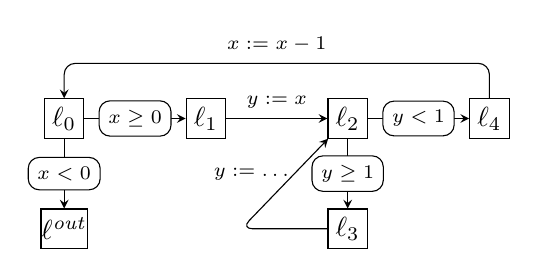
\begin{tikzpicture}[x=1.8cm,y=1.4cm]
		\node[det] (init) at (0,0) {$\loc_0$};
		\node[det] (fin) at (0,-1) {$\loc^{\lout}$};
		\node[det] (as1) at (1,0) {$\loc_1$};
		\node[det] (inner) at (2,0) {$\loc_2$};
		\node[det] (as2) at (2,-1) {$\loc_3$};
		\node[det] (as3) at (3,0) {$\loc_4$};
%		
		\draw[tran] (init) to node[font=\scriptsize,draw, fill=white, 
		rectangle,pos=0.5] {$x<0$} (fin);
		\draw[tran] (init) to node[font=\scriptsize,draw, fill=white, 
		rectangle,pos=0.5] {$x\geq 0$} (as1);
		\draw[tran] (as1) -- node[auto,font=\scriptsize] {$y:=x$} (inner);
		\draw[tran] (inner) to node[font=\scriptsize,draw, fill=white, 
		rectangle,pos=0.5] {$y<1$} (as3);
		\draw[tran] (inner) to node[font=\scriptsize,draw, fill=white, 
		rectangle,pos=0.5] {$y\geq 1$} (as2);
		\draw[tran,rounded corners] (as2) -- (1.25,-1) -- 
		node[font=\scriptsize, 
		label={[xshift=-0.4cm,yshift=-0.2cm,font=\scriptsize] 
		{$y:=\dots$}}] 
		{} 
		(inner);
		\draw[tran, rounded corners] (as3) -- (3,0.5) -- node[font=\scriptsize, 
		label={[font=\scriptsize, yshift=-0.1cm] {$x:=x-1$}}] {} (0,0.5) -- 
		(init);
		\end{tikzpicture}
		%	\hspace{1cm}
		%	\usebox{\uniintt}
		\caption{Example for slicing illustration: program and its pCFG.}
		\label{fig:uniint4}
	\end{subfigure}
	\hspace{0.5cm}
	\begin{subfigure}{0.45\textwidth}
	\usebox{\unintthree}
	%	\hspace{1cm}
	%	\usebox{\uniintt}
	\caption{Program where the outer loop does not have a PVSM that 
		typechecks.}
	\label{fig:uniint2}
	\end{subfigure}
\caption{Program illustrations.}
\label{fig:comp-ex}
\end{figure}

Indeed, taking a closer look at typesystem in~\cite{HolgerPOPL}, there are several reasons for typechecking of PVSM to fail. The major ones are:
\begin{compactenum}
\item
A PVSM $\lem$ for \PP{} $\program$ will not typecheck if $\program$ has a 
nested loop in which the value of $\lem$ can change unboundedly in a single 
step (see Figure~\ref{fig:uniint}). 
\item
A PVSM $\lem$ for  \PP{} $\program$ will not typecheck if $\program$ has a 
nested loop which itself has a nested loop in which some variable appearing in 
some expression in $\lem$ is modified, see 
Figure~\ref{fig:uniint2}.\footnote{Both these statements regarding typechecking 
failure are somewhat simplified, even in these two cases the PVSM might 
sometimes typecheck correctly, in case where the nested loops are followed by 
assignments which completely overwrite the effect of these loops, e.g. if 
the program in Figure~\ref{fig:uniint2} contained an assignment $x:=0$. 
However, the statements intuitively 
summarize the major reasons for typechecking failure. }
\end{compactenum}



Thus, the typechecking algorithm may rule out programs where the termination-controlling variable represents e.g. a length of an array, which can be doubled/halved in some sub-program do to (de)allocation, merging, or splitting.
To overcome the rather strict typechecking, we use the results on LexRSMs to define a new notion of compositional ranking supermartingales, which we call \emph{nob-negative compositional (NC)} supermartingales. For the sake of generality, we allow NC martingales to be general measurable maps, not necessarily propositionally linear.

\begin{definition}
\label{def:nonneg-comp}
A 1-dimensional measurable map $\lem$ is an NC supermartingale (NCSM) for a program $\program$ supported by an invariant map $\inv$ if there exists $\eps>0$ such that $\lem$ is:
\begin{compactenum}
\item  $\inv$-non-negative in each location of $\pCFG_{\program}$;
\item 
 $\eps$-$\inv$-ranking in each location $\loc\in\slice{(\program)}$; and
\item 
  $\inv$-unaffected in each $\loc\in\loops(\program)$.
\end{compactenum}
A (propositionally) linear NCSM (LinNCSM) is a NCSM which is also a (propositionally) linear expression map.
\end{definition}



We can prove that NCSMs are a sound method for proving a.s. termination in a compositional way, without any additional assumptions.

\begin{theorem}
\label{thm:nonneg-comp}
Let $\program$ be a \PP{} of the form $\textbf{while } \Psi \textbf{ do } 
\programbody \textbf{ od}$. Assume that each nested loop of $\program$ 
terminates almost surely from each reachable configuration, and that there 
exists a NCSM for $\program$ supported by some invariant map. Then $\program$ 
terminates almost surely from each initial configuration.
\end{theorem}
\begin{proof}[Proof (Key Idea)]
Assume that there is set of non-terminating runs $A$ of positive probability.
Let $\{X_i\}_{i=0}^{\infty}$ be a stochastic process returning the value of 
NCSM $\lem$ in step $i$. We show that for each $i$ it holds $\E[X_i] 
\leq \lem(\locinit,\vecinit) - \eps\cdot \E[\sharp_i]$, where $\sharp_i$ is the 
random variable returning the number of times a location from 
$\slice(\program)$ is visited. Since all sub-loops of $\program$ terminate 
a.s., $\lim_{i\rightarrow \infty}\sharp_i(\run)=\infty$ for $\run\in A$. Since 
$A$ has positive probability $\lim_{i\rightarrow 
\infty}\E[\sharp_i(\run)=\infty]$, it holds $\lim_{i\rightarrow 
\infty}\E[X_i] = -\infty$, a contradiction with non-negativity of $\lem$.
\end{proof}

Hence, NCSMs effectively trade the uniform integrability condition for 
non-negativity over the whole program. We believe that the latter condition is 
substantially easier to impose and check automatically, especially in the case 
of affine probabilistic programs and (propositionally) linear NCSMs: for 
\APP{}s, synthesizing NCSM entails synthesizing sufficient program invariants 
(for which there is a good automated tool support~\cite{FG10:aspic})  encoding 
the ranking, 
unaffection, and non-negativity conditions into a collection of linear 
constraints (as for general LinLexRSMs in Section~\ref{sec:algo}). 
Figures~\ref{fig:uniint} and~\ref{fig:uniint2} show instances where attempts to 
to prove of a.s. termination via PVSMs fail while proofs via LinNCSMs work. 

\begin{example}
For all programs in Figures~\ref{fig:uniint} and~\ref{fig:uniint2} there are 
LinNCSMs for all the loops in the program, which shows that the programs 
terminate 
a.s. In Figure~\ref{fig:uniint}, for both programs the inner loops have 
LinNCSMs of the form $c+d_{\loc}$, for $d_{\loc}$ a location-specific constant, 
while the outer loops have LinNCSMs of the form $x+d_{\loc}'$. In 
Figure~\ref{fig:uniint2} the program similarly has LinNCSMs defined, proceeding 
from the innermost loop and neglecting the location-specific constants, by 
variables $z$, $y$, $x$.
\end{example}
%While we defined NCSMs as one-dimensional measurable maps to make them analogous to 

Using LinNCSMs we can devise the following simple algorithm for compositional proving of almost-sure termination of \APP{}s:

\begin{algorithm}
\SetKwInOut{Input}{input}\SetKwInOut{Output}{output}
\DontPrintSemicolon

\Input{An \APP{} $\program$ together with an invariant map $\inv$.}
$d\leftarrow \text{ depth of loop nesting in $\program$}$\;
\For{$i \leftarrow d$ \KwTo $0$}{
\ForEach{sub-loop $\program'$ of $\program$ nested $i$ levels below the main loop}{
\label{algoline:one}
$\linsystem \leftarrow$ system of lin. constraints encoding the existence of LinNCSM for $\program'$ supported by $\inv$\;
\label{algoline:two}\If{$\linsystem$ not solvable}{check existence of a PVSM for $\program'$~\cite{HolgerPOPL}
\;
\lIf{PVSM does not exist}{\Return{``cannot prove a.s. termination of $\program$''}}
}
}
}
\Return{``$\program$ terminates a.s.'' }
\caption{Compositional Termination Proving}
\label{algo:compositional}
\end{algorithm}

The soundness of the algorithm follows from Theorems~\ref{thm:nonneg-comp} and 
\ref{thm:holger-comp}. Note that we use the PVSM-based algorithm 
of~\cite{HolgerPOPL} as a back-up sub-procedure for the case when LinNCSM-based 
proof fails. Hence, Algorithm~\ref{algo:compositional} can compositionally 
prove a.s. termination of strictly larger class of programs than the PVSM-based 
algorithm alone.

To summarize, the novelty of NCSMs is the following:
\begin{compactenum}
\item
NCSMs allow compositional, fully automated proofs of a.s. termination without the need for reasoning about uniform integrability.
\item LinNCSMs are capable of proving a.s. termination of programs for which no uniformly integrable PVSMs exist (and hence the method of~\cite{HolgerPOPL} cannot be used at all on such programs).
\item LinNCSMs are capable of proving a.s. termination of programs for which the method of~\cite{HolgerPOPL} cannot be applied in an automated way, do to failure of the typechecking procedure.
\end{compactenum}

\subsection{Multidimensional Compositional Ranking}

As noted previously, a fundamental advantage of LexRSMs over PVSMs is that LexRSMs can handle loops that go through several computational phases and as a result of this do not admit one-dimensional ranking supermartingales. Above, we defined NCSMs as one-dimensional objects, to make them analogous to PVSMs for better comparison. However, we can also define a multi-dimensional version of NCSMs. We say that, given an invariant map $\inv$, an $n$-dimensional measurable map is $\inv$-ranking in a location $\loc$ if for each $\vec{x}\in \inv(\loc)$ there exists $1\leq j \leq n$ such that $\preexp{\lem_j}(\loc,\vec{x}) \leq \lem_j(\loc,\vec{x})-\eps$ and for each $j'<j$ the map $\lem_{j'}$ is $\inv$-unaffected in $\loc$.

\begin{definition}
An $n$-dimensional measurable map $\vec{\lem}=(\lem_1,\dots,\lem_n)$ is an NC supermartingale (NCSM) for a program $\program$ supported by an invariant map $\inv$ if there exists $\eps>0$ such that:
\begin{compactenum}
	\item  for each $1\leq i \leq n$, $\lem_i$ is non-negative in each location of $\pCFG_{\program}$;
	\item 
	$\vec{\lem}$ is $\eps$-ranking in each location $\loc\in\slice{(\program)}$; and
	\item 
	for each $1\leq i \leq n$, $\lem_i$ is
	unaffected in each $\loc\in\loops(\program)$.
\end{compactenum}
An $n$-dimensional (propositionally) linear NCSM (LinNCSM) is an $n$-dimensional NCSM which is also a (propositionally) linear expression map.
\end{definition}

The following theorem can be proved in the same way as Theorem~\ref{thm:nonneg-comp}.

\begin{theorem}
Let $\program$ be a \PP{} of the form $\textbf{while } \Psi \textbf{ do } 
\programbody \textbf{ od}$. Assume that each nested loop of $\program$ terminates almost surely from each reachable configuration, and that there exists a NCSM for $\program$ supported by some invariant map. Then $\program$ terminates almost surely.
\end{theorem}

For \APP{}s, we can generalize Algorithm~\ref{algo:compositional} by changing line~\ref{algoline:one} to ``check existence of a multi-dimensional LinNCSM for $\program'$'' and line~\ref{algoline:two} to ``\textbf{if} a multi-dimensional LinNCSM does not exist.'' The check of existence of a multi-dimensional LinNCSM for $\program'$ can be done by algorithm presented in Section~\ref{xxx}, modified so as to only pursue ranking for transitions outgoing from locations belonging to $\slice(\program')$. (I.e., only these transitions have $\eps_{\tau}$ included in the objective function, and algorithm terminates once all such transitions are ranked.) This further expands the usage of the algorithm.

There are several advantages of using LexRSMs in a compositonal way. First, using Algorithm~\ref{algo:compositional} (modified for multi-dimensional LinNCSMs) we opt for solving a larger number of smaller linear systems rather than a smaller number of larger ones, which may be sometimes advantageous for performance reasons. Second, using compositional reasoning, we can leverage LexRSMs in a situation where some of the sub-loops were already proved to be a.s. terminating by some other argument, such as using an interactive proof assistant that leverages human intuition. This makes the LexRSM method applicable to programs whose parts are difficult to treat via automated static analysis.


%% I SHOULD MAYBE EXPLAIN THAT THE NEED TO PERFORM A STATIC ANALYSIS OF THE WHOLE PROGRAM IS 
%% NOT LIMITING, AS SOMETHING SIMILAR NEEDS TO BE DONE FOR PVSM. BUT MAYBE LEAVE THIS FOR REBUTTAL. :)

%Each measurable map for $\lem$ can be, in a natural way, restricted to a 
%measurable map $\lem_{\program'}$ for $\program'\in \loops(\program)$, 
%since each pCFG $\pCFG_{\program'}$ is a sub-pCFG of $\pCFG_{\program}$. 
%Similarly, a measurable map $\lem$ for $\program$ can be restricted to a 
%measurable map $\lem_{\slice}$ for $\slice(\program)$, since 
%$\pCFG_{\slice(\program)}$ is produced from $\pCFG_{\program}$ essentially by 
%removing certain locations (provided that we identify the locations forming 
%heads of nested loops with locations preceding skip statements), and 
%$\lem_{\slice}$ is defined to be equal to $\lem$ in all the locations that 
%remained. Similarly, 


\section{Bounds on Expected Termination Time}

As shown in Example~\ref{ex:infinite-time}, already LinLexRSM maps are capable 
of proving almost-sure termination of programs whose expected termination time 
is infinite. However, it is often desirable to obtain bounds on expected 
runtime of a program. In this section, we present a LexRSM-based proof rule for 
obtaining bounds on expected runtime, and we show how to automatize the usage 
of this proof rule to obtain bounds on expected runtime in a 
subclass of \PP{}s.

As in the case of a.s. termination we start with general mathematical statement 
about LexRSMs. We define a restricted class of strict LexRSMs with \emph{bounded 
expected conditional increase} property. Recall from 
definition~\ref{def:lexrsm} that strict
LexRSM for a stopping time $\stime$ is characterized by the possibility to 
a.s. partition, for each $i\in \Nset_0$, the set $\{\omega\in \Omega\mid 
\stime(\omega)>i \}$ into $n$ sets $L^i_1,\dots,L^i_d$ such that, intuitively, 
on $L^i_j$ the conditional expectation of $\vec{X}_{i+1}[j]$ given $\genfilt_i$ 
is smaller than $\vec{X}_i[j]$, and for all $j'<j$, on $L^i_{j'}$ the 
conditional expectation of $\vec{X}_{i+1}[j]$ given $\genfilt_i$ 
is no larger than $\vec{X}_i[j]$. This leaves the opportunity of conditional 
expectation of $\vec{X}_{i+1}[j]$ being larger than $\vec{X}_i[j]$ on 
$L^i_{j''}$ with $j''>j$. The conditional expected increase property bounds the 
possibility of this increase.

\begin{definition}
	\label{def:lexrsm-eci}
Let $\{\vec{X}_{i}\}_{i=0}^{\infty}$ be an 
$n$-dimensional strict LexRSM for some stopping time $\stime$, defined w.r.t. some 
filtration $\{\genfilt_i\}_{i=0}^{\infty}$. We say that 
$\{\vec{X}_{i}\}_{i=0}^{\infty}$ has \emph{$\vec{c}$-bounded expected 
conditional 
increase (ECI),} for 
some non-negative vector $\vec{c}\in\Rset^d$, if there exists an instance $(\{\vec{X}_{i=0}^{\infty},\{L_1^i,\dots,L_{n+1}^i\}_{i=0}^{\infty})$ of the strict LexRSM (i.e. $L^i_{n+1}=\emptyset$ for all $i$) such that for each $i\in \Nset_0 $ and 
each $1\leq 
j \leq n $ it holds 
$\E[\vecseq{X}{i+1}{j}\mid \genfilt_i]\leq \vecseq{X}{i}{j}+\vec{c}[j]$ on 
$L^i_{j''}$, 
for all $j''>j$ 
(here $L^i_1,\dots,L^i_n$ are as in Definition~\ref{def:lexrsm}).
\end{definition}

For strict LexRSMs with $\vec{c}$-bounded ECI we have the following result. For 
simplicity, 
we formulate the result for 1-LexRSMs, though it is easy to prove analogous 
result for general $\eps$-LexRSMs, $\eps>0$, at the cost of obtaining less 
readable formula.

\begin{theorem}
\label{thm:runtime-bound}
\label{THM:RUNTIME-BOUND}
Let $\{\vec{X}_{i}\}_{i=0}^{\infty}$ be an 
$n$-dimensional strict LexRSM with $c$-bounded ECI for some stopping time $\stime$. 
Then $\E[\stime]\leq  
\sum_{j=1}^{n}\E[\vecseq{X}{0}{j}]\cdot(1+\sum_{j'= j+1}^{n}\prod_{j'}^{n} 
\vec{c}[j'])$.
\end{theorem}
\begin{proof}
Fix an instance $(\{\vec{X}_{i=0}^{\infty},\{L_1^i,\dots,L_{n+1}^i\}_{i=0}^{\infty})$ satisfying Definition~\ref{def:lexrsm-eci}. Denote $\noofdecrank_j(\omega)$ the number of steps $i$ in which $\omega\in 
L_j^i$. Since by Theorem~\ref{thm:lexrsm-main} the existence of strict LexRSM entails 
$\probm(\stime<\infty)=1$, the value $\noofdecrank_j(\omega)$ is a.s. finite for all $1\leq j \leq n$. 
We prove that for each $1\leq j \leq n$ it holds $\E[\noofdecrank_j]\leq 
\vec{c}[j]\cdot\left(\sum_{j'<j}\E[\noofdecrank_{j'}]\right) + 
\E[\vecseq{X}{0}{j}].$ Since $\stime(\omega)=\sum_{1\leq j \leq n} 
\noofdecrank_j(\omega)$, for each $\omega\in \Omega$ (and hence, due to 
linearity of expectation $\E[\stime]=\sum_{1\leq j \leq n} 
E[\noofdecrank_j]$), the statement of the 
Theorem follows by an easy induction. 

To prove the required inequality, let $\nodecrank{k}{j}(\omega)$ be the number 
of steps $i$ \emph{within the first $k$} steps such that $\omega\in L_j^i$. We 
prove, by induction on $k$, that for each $k$ it holds 
$\E[\nodecrank{k}{j}]\leq 
\vec{c}[j]\cdot\left(\sum_{j'<j}\E[\nodecrank{k}{j'}] \right)+ 
\E[\vecseq{X}{0}{j}] - \E[\vecseq{X}{k}{j}]$. Once this is proved, the 
desired inequality follows by taking $k$ to $\infty$, since 
$\lim_{k\rightarrow \infty}\E[\nodecrank{k}{j}] = \E[\noofdecrank_j]$ and 
$\lim_{k\rightarrow \infty}\E[\vecseq{X}{k}{j}] \geq 0$. The inductive proof is 
somewhat technical and deferred to \AppendixMaterial.

%The base case $k=0$ is simple as both sides of the inequality are zero. Assume 
%that the inequality holds for some $k\geq 0$. We have 
%$\E[\nodecrank{k+1}{j}]=\E[\nodecrank{k}{j}]+\probm{(L_j^{k})}$, so from 
%induction hypothesis we get 
%\begin{equation}
%\label{eq:time1}
%\E[\nodecrank{k+1}{j}]\leq 
%\vec{c}[j]\cdot\left(\sum_{j'<j}\E[\nodecrank{k}{j'}] \right)+ 
%\E[\vecseq{X}{0}{j}] - \E[\vecseq{X}{k}{j}] + \probm{(L_j^{k})}.\end{equation} 
%Now denote 
%$L^k_{<j} = L^k_1 \cup \dots\cup L^k_{j-1}$ and $L^k_{>j}= 
%L^k_{j+1}\cup\dots\cup L^k_{d}$. We have  
%$\E[\vecseq{X}{k}{j}] = \E[\vecseq{X}{k}{j}\cdot 
%\indicator{ L_{<j}^k}] + \E[\vecseq{X}{k}{j}\cdot 
%\indicator{ L_j^k}] + \E[\vecseq{X}{k}{j}\cdot 
%	\indicator{L_{>j}^k}] \geq 
%\E[\vecseq{X}{k+1}{j}\cdot 
%	\indicator{ L_{<j}^k}] -\vec{c}[j]\cdot \probm(L_{<j}^k) + 
%	\E[\vecseq{X}{k+1}{j}\cdot 
%	\indicator{ L_{j}^k}] + \probm(L_{j}^k) + \E[\vecseq{X}{k+1}{j}\cdot 
%	\indicator{ L_{>j}^k}]= \E[\vecseq{X}{k+1}{j}] -\vec{c}[j]\cdot 
%	\probm(L_{<j}^k)+ \probm(L_{j}^k)$. Plugging this 
%	into~\ref{eq:time1} yields
%\begin{align*}
%\E[\nodecrank{k+1}{j}]&\leq 
%\vec{c}[j]\cdot\left(\sum_{j'<j}\E[\nodecrank{k}{j'}] \right)+ 
%\E[\vecseq{X}{0}{j}] - \E[\vecseq{X}{k+1}{j}] + \vec{c}[j]\cdot 
%\probm(L_{<j}^k)\\
%&=\vec{c}[j]\cdot\left(\sum_{j'<j}\E[\nodecrank{k+1}{j'}] \right)+ 
%\E[\vecseq{X}{0}{j}] - \E[\vecseq{X}{k+1}{j}].
%\end{align*}
%
%\end{align}
\end{proof}

To transfer this mathematical result to probabilistic programs, we want to 
impose a restriction on LexRSM maps that ensures that all components of a 
LexRSM map have, from each reachable configuration, an expected one-step 
increase of at most $c$. Here $c$ can be a constant, but it can also be a value 
that depends on the initial configurations: this is to handle cases where some 
variables are periodically reset to a value related to the initial variable 
values, such as variable $y$ in Figure~\ref{fig:uniint4}. To this end, let 
$\program$ be a \PP{} with a pCFG $\pCFG_\program$ and let 
$\vec{\lem}=(\lem_1,\dots,\lem_n)$ be an 
$n$-dimensional $1$-LexRSM map for $\program$. Consider an $n$-dimensional 
vector 
$\vec{\bar{c}}=(\bar{c}_1,\dots,\bar{c}_n)$ whose each component is an 
expression over variables of 
$\program$. We say 
that $\vec{\lem}$ has 
$\vec{\bar{c}}$-bounded ECI w.r.t. invariant map $\inv$ if the following holds 
for each initial configuration $(\locinit,\vecinit)$ with $\vecinit\in 
\vecinitset$: for 
each 
configuration $(\loc,\vec{x})$ with $\vec{x}\in \inv(\loc)$ and generalized 
transition $\tilde{\tau}$ 
of 
$\pCFG_\program$ outgoing from $(\loc,\vec{x})$ it holds that if $j$ is 
the smallest index such that 
$\tilde{\tau}$ is $1$-ranked by $\lem_j$ from $(\loc,\vec{x})$, then for all 
$j'>j$ the gen. transition $\tilde{\tau}$ is $f$-ranked by $\lem_{j'}$ from 
$(\loc,\vec{x})$, where $f=-c_{j'}(\vecinit)$. From 
Theorem~\ref{thm:runtime-bound} we have the following:

\begin{corollary}
\label{col:runtime-progs}
Let $\program$ be a probabilistic program. Assume that there exists an 
$n$-dimensional $\eps$-LexRSM map $\vec{\lem}=(\lem_1,\dots,\lem_d)$ for 
$\program$ supported 
by some 
invariant map $\inv$, scuh that $\vec{\lem}$ has $\vec{\bar{c}}$-bounded ECI 
(w.r.t. $\inv$) 
for some vector of expressions $\vec{\bar{c}}=(\bar{c}_1,\dots,\bar{c}_n)$. 
Then under each scheduler $\sigma$ and for each initial valuation of program 
variables $\vecinit\in\vecinitset$ it holds $\E^{\sigma}_{\vecinit}[\ttime]\leq
\sum_{j=1}^{n}\lem_j(\locinit,\vecinit)\cdot(1+\sum_{j'= j+1}^{n}\prod_{j'}^{n} 
\bar{c}_{j'}(\vecinit)).$
%\sum_{j=1}^{n}\lem_j(\locinit,\vecinit)\cdot(\bar{c}_j(\vecinit))^{n-j}$.
\end{corollary}

\begin{example}
Consider the program in Figure~\ref{fig:uniint4}. For the program we have an 
invariant map $\inv$ with $\inv(\loc_0)=x\geq -1$, $\inv(\loc_1)=\inv(\loc_4) = 
x\geq 0 
\wedge z\geq 0$, $\inv(\loc_2)=\inv(\loc_3)= x\geq 0 \wedge y \geq 0
\wedge z\geq 0$, and $\inv(\loc^{\lout})=\mathit{true}$. Further, there exists 
the following 
$3$-dimensional 
$1$-LinLexRSM map $\vec{\lem}$ supported by $\inv$: 
$\vec{\lem}(\loc_0)=(2x+3,0,2)$, $\vec{\lem}(\loc_1)=(2x+3,0,1)$, 
$\vec{\lem}(\loc_2)=(2x+2,y,1)$, $\vec{\lem}(\loc_3)=(2x+2,y,0)$, 
$\vec{\lem}(\loc_4)=(2x+2,0,0)$, and $\vec{\lem}(\loc^{\lout})=(0,0,0)$. It is 
easy to check that $\vec{\lem}$ is has $(0,z,2)$-bounded ECI. Applying 
Corollary~\ref{col:runtime-progs} yields $\E[\ttime]\leq (2x_{\mathit{init}} + 
3)\cdot(1+3z_{\mathit{init}})+0+2= 6x_{\mathit{init}}z_{\mathit{init}} + 
2x_{\mathit{init}} + 9z_{\mathit{init}}+5$. Note that this quadratic bound is 
asymptotically optimal for the given program.
\end{example}

Now assume that we have synthesized a $1$-LexRSM map $\vec{\lem}$ and we want 
to check if there exists $\bar{\vec{c}}$ such that $\vec{\lem}$ has 
$\bar{\vec{c}}$-bounded ECI. In the linear setting (i.e. the program is an 
\APP{}, masp $\lem$ and $\inv$ are linear, and we seek $\vec{\bar{c}}$ which is 
a vector of affine expressions) we can encode the existence of $\vec{\bar{c}}$ 
into a system of linear inequalities in the similar way as the existence of a 
linear LexRSM maps was encoded in Section~\ref{sec:lex-programs}. That is, we 
set up a linear template with unknown coefficients for each component of 
$\vec{\bar{c}}$ and using Farkas's lemma we set up a system of linear 
constraints, which includes the unknown coefficients as variables, encoding the 
fact that $\vec{\lem}$ has $\bar{\vec{c}}$-bounded ECI. Details are provided 
in~\AppendixMaterial. In this way, we can check in polynomial time if 
Corollary~\ref{col:runtime-progs} can be applied to $\vec{\lem}$, and if yes, 
we can synthesize the witness vector $\bar{\vec{c}}$. Since $\bar{\vec{c}}$ 
consists of affine expressions, Corollary~\ref{col:runtime-progs} provides a 
polynomial (in the size of 
initial variable valuation) upper bound on expected runtime.

%\textbf{[PETR: FINISH THIS SECTION]}


%\input{martingale-use}
%\input{repulsing-use}
%\input{effectivity}
%\input{alg}
%%\input{syntax}
%%\input{semantics}
%%\input{termination}
%%\input{term-complexity}
%%\input{concentration-complexity}
%%\input{concentration}
%\input{experiment}

\section{Related Work}
In this section we discuss the related works.

\smallskip\noindent{\em Probabilistic programs and termination.}
In early works the termination for concurrent probabilistic programs was studied 
as fairness~\cite{SPH84}, which ignored precise probabilities.
For countable state space a sound and complete characterization of almost-sure termination 
was presented in~\cite{HS85}, but nondeterminism was absent.
A sound and complete method for proving termination of finite-state programs
was given in~\cite{EGK12}.
For probablistic programs with countable state space and without 
nondeterminism, the {\em Lyapunov ranking functions} provide a sound and 
complete method to prove positive termination~\cite{BG05,Foster53}.
For probabilistic programs with nondeterminism, but restricted to discrete probabilistic
choices, the termination problem was studied in~\cite{MM04,MM05}.
The RSM-based (ranking supermatingale-based) approach extending ranking functions was first 
presented in~\cite{SriramCAV} for probabilistic programs without non-determinism,
but with real-valued variables, and its extension for probabilistic programs
with non-determinism has been studied in~\cite{HolgerPOPL,CFNH16:prob-termination,CAV-POLY,POPL,ARXIV}.
While all these results deeply clarify the role of RSMs for probabilistic programs, 
the notion of lexicographic RSMs to obtain a practical approach for termination 
analysis for probabilistic programs has not been studied before, which we consider in 
this work.


\smallskip\noindent{\em Other approaches.}
Besides RSMs, other approaches has also been considered for probabilistic programs.
A sound approach~\cite{DBLP:conf/sas/Monniaux01} for almost-sure termination 
is to explore the exponential decrease of probabilities upon bounded-termination 
through abstract interpretation~\cite{DBLP:conf/popl/CousotC77}.
MENTION PROOF RULES AND NOT AN AUTOMATED APPROACH.



\smallskip\noindent{\em Non-probabilistic programs.}
Termination analysis of non-probabilistic programs has also been extensively 
studied~\cite{DBLP:conf/cav/BradleyMS05,DBLP:conf/tacas/ColonS01,DBLP:conf/vmcai/PodelskiR04,DBLP:conf/pods/SohnG91,BMS05b,CSZ13,LJB01}.
Ranking functions are at the heart of the termination analysis, and lexicographic 
ranking function has emerged as one of the most efficient and practical approaches
for termination analysis~\cite{}.
In this work we extend such lexicographich ranking functions to probabilistic programs,
and present lexicographic RSMs for almost-sure termination analysis of probabilistic programs
with non-determinism.



\section{Conclusion and Future Work}
In this work we considered lexicographic RSMs for termination analysis of probabilistic
programs with nondeterminism.
We showed it presents a sound approach for almost-sure termination, that is compositional,
algorithmically efficient, and leads to approach that can handle realistic programs.
There are several interesting directions of future work.
Lexicographic ranking functions has been considered in several works to 
provide different practical methods for analysis of non-probabilistic programs.
First, while our work presents the foundations of lexicographic RSMs for probabilistic 
programs, extending other practical methods of lexicographic ranking functions to 
lexicographic RSMs is an interesting direction of future work.
Second, while our algorithmic approaches focus on the linear case, it would be interesting
to consider other non-linear, and polynomial functions in the future.







%{\scriptsize
\bibliographystyle{ACM-Reference-Format}
\bibliography{bibliography-master,new-popl18}
%}
%\clearpage
%\appendix

%\begin{center}
%{\Large Supplementary Material}
%\end{center}

%\input{app-def}

%%\nouppercaseheads
%\def\@secfont{\sffamily\bfseries}
\section{Details of Program Syntax}
In this subsection we present the details of the syntax of (affine) 
probabilistic 
programs.

Recall that $\vars$ %and $\mathcal{R}$ 
is a collection of 
\emph{variables}.
%and \emph{random} variables, respectively. 
Moreover, let $\mathcal{D}$ be a set of \emph{probability distributions} on 
real numbers.
The abstract syntax of affine
probabilistic programs (\APP s)
is given by the grammar in Figure~\ref{fig:syntax}, where
the expressions $\langle \mathit{pvar}\rangle$ and $\langle
\mathit{dist}\rangle$  range over $\vars$ and $\mathcal{D}$, respectively.
We allow for non-deterministic assignments, expressed by a statement $x:=
\text{\textbf{ndet($\mathit{dom}$)}}$, where $\mathit{dom}$ is a \emph{domain
specifier} determining the set from which the value can be chosen: for general 
programs it can be any Borel-measureable set, for \APP{}s it has to be an 
interval (possibly of infinite length).  
The grammar is such that $\langle \mathit{expr} \rangle$ %and $\langle
%\mathit{rexpr} \rangle$ 
may evaluate to an arbitrary affine expression over the
program variables.
%, and the program and random variables, respectively (note that
%random variables can only be used in the RHS of an assignment). 
Next, $\langle
\mathit{bexpr}\rangle$ may evaluate to an arbitrary propositionally linear
predicate. 

For general (not necessary affine) \PP{}s we set $\langle\mathit{expr}\rangle$ 
to be the set of all expressions permitted by the set of mathematical 
operations of the underlying language. Similarly, $\langle\mathit{bexpr} 
\rangle$ is the set of all predicates, as defined in Section~\ref{sec:prelim}.

The guard of each if-then-else statement is either $\star$, 
representing a (demonic) non-deterministic choice between the branches,
a keyword \textbf{prob}($p$), where $p\in [0,1]$ is a number given in decimal
representation (represents a probabilistic choice, where  the if-branch is
executed with probability $p$ and the then-branch with probability $1-p$), or
the guard is a propositionally linear predicate, in which case the statement
represents a standard deterministic conditional branching.

%We assume that each \APP{} $\program$ is preceded by an initialization 
%preamble 
%in 
%which 
%each variable appearing in $\program$ is assigned some concrete number. 
Regarding distributions, for each $d\in \mathcal{D}$ we assume the
existence of a program primitive denoted by '\textbf{sample($d$)}' implementing 
sampling from $d$. In practice, the distributions appearing in a program would 
be those for which sampling is 
provided by suitable libraries (such as 
uniform distribution over some interval, Bernoulli, geometric, etc.), 
but we 
abstract away from these implementation details. For the purpose of our 
analysis, it is sufficient that for each distribution $d$ appearing in the 
program the following characteristics: expected value $\expv[d]$ of $d$ and a 
set $SP_d$ containing \emph{support} of $d$  (the support of $d$ is the 
smallest 
closed set of real numbers whose complement has probability zero 
under $d$). \footnote{In 
particular, 
a support of a \emph{discrete} probability 
distribution $d$ is simply the at most countable set of all points on a real 
line that have positive probability under $d$. For continuous distributions, 
e.g. a normal distribution, uniform, etc., the support is typically either 
$\Rset$ or some closed real interval. } For \APP{}s, $SP_d$ is required to be 
an 
interval. 
\begin{figure}
\begin{align*}
\langle \mathit{stmt}\rangle &::= 
%\,\langle\mathit{pvar}\rangle
%\,\text{'$:=$'}\, \langle\mathit{rexpr} \rangle \mid 
%\langle\mathit{pvar}\rangle \,\text{'$:=$}\,
%\text{\textbf{ndet($\langle\mathit{dom}\rangle$)}'}  \\
\langle \mathit{assgn} \rangle \mid \text{'\textbf{skip}'} \mid 
\langle\mathit{stmt}\rangle \, \text{';'} \, \langle \mathit{stmt}\rangle \\
%
&\mid   \text{'\textbf{if}'} \,
\langle\mathit{ndbexpr}\rangle\,\text{'\textbf{then}'} \, \langle
\mathit{stmt}\rangle \, \text{'\textbf{else}'} \, \langle \mathit{stmt}\rangle
\,\text{'\textbf{fi}'}
\\
%
&\mid  \text{'\textbf{while}'}\, \langle\mathit{bexpr}\rangle \,
\text{'\textbf{do}'} \, \langle \mathit{stmt}\rangle \, \text{'\textbf{od}'}
\\
\langle \mathit{assgn} \rangle &::= 
\,\langle\mathit{pvar}\rangle
\,\text{'$:=$'}\, \langle\mathit{expr} \rangle \mid 
\langle\mathit{pvar}\rangle \,\text{'$:=$}\,
\text{\textbf{ndet($\langle\mathit{dom}\rangle$)}'}
\\
&\mid \langle\mathit{pvar}\rangle \,\text{'$:=$}\,
\text{\textbf{sample($\langle\mathit{dist}\rangle$)}'}
%
%
%
%
%&
%
%\\
%
%\\
\\
\vspace{0.5\baselineskip}
%\\
%\langle\mathit{var} \rangle &::= \langle\mathit{pvar} \rangle \mid 
%\langle\mathit{rvar}\rangle
%\\
%%\vspace{\baselineskip}
%\vspace{0.5\baselineskip}
%\\
\langle\mathit{expr} \rangle &::= \langle \mathit{constant} \rangle \mid
\langle\mathit{pvar}\rangle
%\\
\mid \langle \mathit{constant} \rangle \,\text{'$\cdot$'} \,
\langle\mathit{pvar}\rangle
\\
%
&\mid \langle\mathit{expr} \rangle\, \text{'$+$'} \,\langle\mathit{expr} \rangle
\mid \langle\mathit{expr} \rangle\, \text{'$-$'} \,\langle\mathit{expr} \rangle
%\\
%%
%\vspace{0.5\baselineskip}
%%\\
%\langle\mathit{rexpr} \rangle &::= \langle\mathit{expr} \rangle \mid 
%\langle\mathit{rvar}\rangle 
%%\mid
%% \langle\mathit{pvar}\rangle 
%\mid\langle\mathit{constant} \rangle \,\text{'$*$'} \,
%\langle\mathit{rvar}\rangle \\
%%
%&\mid
%%\langle\mathit{constant} \rangle \,\text{'$*$'} \, \langle\mathit{pvar}\rangle
%%\mid 
%\langle\mathit{rexpr} \rangle\, \text{'$+$'} \,\langle\mathit{rexpr} \rangle
%\mid \langle\mathit{rexpr} \rangle\, \text{'$-$'} \,\langle\mathit{rexpr}
%\rangle
%%\\
%%\vspace{0.5\baselineskip}
%%\\ \langle\mathit{bexpr} \rangle &::= \langle \mathit{predicate}\rangle \mid 
%%\neg \langle\mathit{predicate}\rangle
\\
%
%\vspace{0.5\baselineskip}
%\langle \mathit{dom} \rangle &::= \text{'\textbf{Int}'} \mid
%\text{'\textbf{Real}'} \mid
%\text{'\textbf{Int}$[\langle\mathit{constant}\rangle,\langle\mathit{constant}\rangle]$'}
% \\ 
%% 
% &\mid
%\text{'\textbf{Real}$[\langle\mathit{constant}\rangle,\langle\mathit{constant}\rangle]$'}
%\mid \langle \mathit{dom} \rangle \text{'\textbf{or}'}\langle \mathit{dom}
%\rangle
%\\
%
%\vspace{0.5\baselineskip}
%\\
\langle \mathit{bexpr}\rangle &::=  \langle \mathit{affexpr} \rangle \mid
\langle \mathit{affexpr} \rangle \, \text{'\textbf{or}'} \,
\langle\mathit{bexpr}\rangle
\vspace{0.5\baselineskip}
\\
%
%\vspace{\baselineskip}
%\\
\langle\mathit{affexpr} \rangle &::=  \langle\mathit{literal} \rangle\mid
\langle\mathit{literal} \rangle\, \text{'\textbf{and}'}
\,\langle\mathit{affexpr} \rangle
\\
%
\langle\mathit{literal} \rangle &::= \langle\mathit{expr} \rangle\,
\text{'$\leq$'} \,\langle\mathit{expr} \rangle \mid \langle\mathit{expr}
\rangle\, \text{'$\geq$'} \,\langle\mathit{expr} \rangle
\\
%
&\mid \neg \langle \mathit{literal} \rangle
\\
%
%\vspace{0.5\baselineskip}
%\\
\langle\mathit{ndbexpr} \rangle &::= {\star}\mid
\text{'\textbf{prob($p$)}'} \mid \langle\mathit{bexpr} \rangle
\end{align*}
\caption{Syntax of affine probabilistic programs (\APP 's).}
\label{fig:syntax}
\end{figure}

%The syntax is such that $\langle \mathit{expr} \rangle$ and $\langle
%\mathit{rexpr} \rangle$ may evaluate to an arbitrary affine expression over the
%program variables, and the program and random variables, respectively (note
%that random variables can only be used in the RHS of an assignment). Next,
%$\langle \mathit{bexpr}\rangle$ may evaluate to an arbitrary disjunction of
%polyhedral constraints (i.e. conjunctions of linear inequalities and equalities
%over the program variables).



%Additionally to the program body generated by the grammar, we assume that each
%program has a preamble in which both program and random variables are declared.
%We assume that every program variable is initialized to some fixed constant
%upon declaration, and that for each of the random variables its
%For random variables we need to suitably specify their distribution in the
%preamble. This amounts to either directly specifying the joint distribution of
%these variables, or stipulating the variables to be stochastically independent
%and specifying a probability distribution for each one of them. We point out
%that the only parameters of the program's random variables that we use in the
%process of deriving ranking supermartingales are their expected values (which
%we assume to be well-defined and finite) and, for deriving concentration
%inequalities, also bounds on their range. \PN{Is this true? Do we not need
%bounds on their range for as termination as well?} The exact distributions are
%only needed for the actual execution of the program.


%\begin{example}\label{ex:prog}
%We present an example of an affine probabilistic program shown in
%Figure~\ref{ex:prob}.
%The program variable is $x$, and there is a while loop, where given a
%probabilistic
%choice one of two statement blocks $Q_1$ or $Q_2$ is executed.
%The block $Q_1$ (resp. $Q_2$) is executed if the probabilistic choice is at
%least
%$0.6$ (resp. less than $0.4$).
%The statement block $Q_1$ (resp., $Q_2$) is an angelic (resp. demonic)
%conditional
%statement to either increment or decrement $x$.
%\lstset{language=affprob}
%\lstset{tabsize=3}
%\newsavebox{\affproblist}
%\begin{lrbox}{\affproblist}
%\begin{lstlisting}[mathescape]
%$x:=0$;
%while $x \geq 0$ do
%	if prob(0.6) then
%		if angel then
%			$x:=x+1$
%		else
%			$x:=x-1$
%		fi
%	else
%		if demon then
%			$x:=x+1$
%		else
%			$x:=x-1$
%		fi
%	fi
%od
%\end{lstlisting}
%\end{lrbox}
%\begin{figure}[t]
%%%\centering
%\usebox{\affproblist}
%\caption{An example of a probabilistic program}\label{ex:prob}
%\end{figure}
%\end{example}


\section{Details of Program Semantics}


\begin{remark}[Use of random variables]
%\label{rem:randuse}
In the paper we sometimes work with random variables 
that are functions of the type $R\colon\Omega \rightarrow S$ for some finite 
set $S$. These can be captured by the definition given in 
Section~\ref{sec:prelim} by identifying the 
elements of $S$ with distinct real numbers.\footnote{This is equivalent to 
saying that a function $R\colon \Omega\rightarrow S$, with $S$ finite, is a 
random variable if for each $s\in S$ the set $\{\omega\in \Omega\mid 
R(\omega)=s\}$ belongs to $\mathcal{F}$.} The exact choice of numbers is 
irrelevant in such a case, as we are not interested in, e.g. computing expected 
values of such random variables, or similar operations. 
\end{remark}


\paragraph*{From Programs to pCFGs}
To every probabilistic program $P$ we can assign a pCFG $\pCFG_P$ whose 
locations correspond to the values of the
program counter of $P$ and whose transition relation captures the behaviour of
$P$. We illustrate the construction for \APP{}s, for general programs it is 
similar. To obtain $\pCFG_{P}$, we first rename 
the variables in $P$ to 
$x_1,\dots,x_n$, where $n$ is the number of distinct variables in the program. 
The
construction of $\pCFG_P$ can be described inductively.
For each program $P$ the pCFG $\pCFG_P$ contains two distinguished
locations, $\ell^{\lin}_{P}$ and $\ell^{\lout}_{P}$, the latter one being always
deterministic, that intuitively represent the state of the program counter
before and after executing $P$, respectively. In the following, we denote by 
$\id_1$ a function such that for each $\vec{x}$ we have 
$\id_{1}(\vec{x})=\vec{x}[1]$.
\begin{compactenum}
\item {\em Deterministic Assignments and Skips.}
For $P= {x_j}{:=}{E}$ where $x_j$ is a program variable and $E$ is an 
expression, or $P = \textbf{skip}$, the pCFG $\pCFG_P$ consists only of
%these two (deterministic) locations
locations $\ell^{\lin}_P$ and $\ell^{\lout}_P$ (first assignment location, 
second one deterministic) and a
transition $(\ell^{\lin}_{P},\ell^{\lout}_P)$. In the first case, 
$\updates(\ell^{\lin}_{P},\ell^{\lout}_P)=(j,E)$.
\item {\em Probabilistic and Non-Deterministic Assignemnts}
For $P= {x_j}{:=}{\textbf{sample($d$)}}$ where $x_j$ is a program variable and 
$d$ is a distribution, the pCFG $\pCFG_P$ consists locations $\ell^{\lin}_P$ 
and $\ell^{\lout}_P$ and a
transition $\tau=(\ell^{\lin}_{P},\ell^{\lout}_P)$ with $\updates(\tau)=(j,d)$. For 
$P= 
{x_j}{:=}{\textbf{ndet($\mathit{dom}$)}}$, the construction is similar, with 
the only transition being $\tau=(\ell^{\lin}_{P}\ell^{\lout}_P)$ and 
$\updates(\tau)=(j,D)$, where 
$D$ is 
the set specified by the domain specifier $\mathit{dom}$.

\item {\em Sequential Statements.}
For $P = Q_1;Q_2$ we take the pCFGs $\pCFG_{Q_1}$, $\pCFG_{Q_2}$ and
join them by identifying the location $\ell^{\lout}_{Q_1}$ with
$\ell^{\lin}_{Q_2}$, putting $\ell^{\lin}_{P}=\ell^{\lin}_{Q_1}$ and
$\ell^{\lout}_{P}=\ell^{\lout}_{Q_2}$.

\item {\em While Statements.}
For $P = \textbf{while $\phi$ do }Q \textbf{ od}$ we add a new deterministic
location $\ell^{\lin}_{P}$ which we identify with $\ell^{\lout}_{Q}$, a new
deterministic location $\ell^{\lout}_{P}$, and transitions
$\tau=(\ell^{\lin}_{P},\ell^{\lin}_{Q})$,
$\tau'=(\ell^{\lin}_{P},\ell^{\lout}_{P})$ such that $G(\tau)=\phi$ and
$G(\tau')=\neg\phi$.

\item {\em If Statements.}
Finally, for $P = \textbf{if $\mathit{ndb}$ then }Q_1 \textbf{ else } Q_2
\textbf{ fi}$ we add a new location $\ell^{\lin}_{P}$ (which is not an 
assignment location) together with two
transitions $\tau_1 = (\ell^{\lin}_{P},\ell^{\lin}_{Q_1})$, $\tau_2 =
(\ell^{\lin}_{P},\ell^{\lin}_{Q_2})$, and we identify the locations 
$\ell^{\lout}_{Q_1}$ and $\ell^{\lout}_{Q_1}$ with $\ell^{\lout}_{P}$. (If both
$Q_j$'s consist of a single statement, we also identify $\ell^\lin_{P}$ with 
$\ell^{\lin}_{Q_j}$'s.) In this
case the newly added location $\ell^\lin_{P}$ is non-deterministic branching if 
and only 
if
$ndb$ is the keyword '$\star$'. If
$\mathit{ndb}$ is of the form $\textbf{prob($p$)}$, the location $\ell^\lin_{P}$
is probabilistic branching with $\probdist_{\ell^\lin_{P}}(\tau_1)=p$ and
$\probdist_{\ell^\lin_{P}}(\tau_2)=1-p$. Otherwise (i.e. if $\mathit{ndb}$ is a
predicate), $\ell^\lin_{P}$ is a deterministic location
with $G(\tau_1)=\mathit{ndb}$ and $G(\tau_2)=\neg \mathit{ndb}$.
\end{compactenum}
Once the pCFG $\pCFG_P$ is constructed using the above rules, we put
$G(\tau)=\textit{true}$ for all transitions $\tau$ outgoing from deterministic
locations whose guard was not set in the process, and finally we add a self-loop
on the location $\ell^{\lout}_P$. This ensures that the assumptions in
Definition~\ref{def:stochgame} are satisfied.
Furthermore note that for pCFG obtained for a program $P$, since the only
branching is if-then-else branching, every location $\loc$ has at most two
successors $\loc_1,\loc_2$.

\def\xx{\ref{prop:conditional-exp-existence}}

\section{Proof of Proposition~\xx}

We first recall the general statement of the Radon-Nikodym theorem. Given two measurable spaces\footnote{A generalization of a probability space where the measure of $\Omega$ does not have to be 1, but any non-negative number or even infinity.} $(\Omega,\genfilt,\mu)$ and $(\Omega,\genfilt,\nu)$, we say that $\nu$ dominates $\mu$, written $\mu<<\nu$ if for all $A\in \genfilt$, $\nu(A)=0$ implies $\mu(A)=0$. Radon-Nikodym theorem states that if both $\mu$ and $\nu$ are sigma-finite (that is, $\Omega$ is a union of countably many sets of finite measure under $\nu$ and $\mu$), then $\mu<<\nu$ implies that there exists an almost-surely unique $\genfilt$-measurable function $f\colon \Omega\rightarrow [0,\infty)$ such that for each $A \in\genfilt$, the Lebesgue integral of the function $f\cdot\indicator{A}$ in measurable space  $(\Omega,\genfilt,\nu)$ is equal to $\mu(A)$. The function $f$ is called a Radon-Nikodym derivative of $\mu$ w.r.t. $\nu$, and we denote in by $\frac{d\mu}{d\nu}$.

Now assume that $X$ is a non-negative real-valued random variable in some probability space $(\Omega,\genfilt,\probm)$ and $\genfilt'$ is a sub-sigma algebra of $\genfilt$. Note that $\probm$ is sigma-finite. Define a measure $\mu$ on $\genfilt'$ by putting $\mu(A)=\E[X\cdot\indicator{A}]$, for each $A\in \genfilt$ (here $\E$ is the expectation operator, i.e. the Lebesgue integral, in probability space $(\Omega,\genfilt',\probm')$, where $\probm'$ is a restriction of $\probm$ to $\genfilt'$). Then $\mu$ is sigma-finite: indeed, for any $n\in \Nset$ let $A_n = \{\omega\in\Omega\mid X(\omega)\leq n\}$. Then $\mu(A_n)\in [0,n]$, in particular it is finite, and since $X$ is real-valued, we have $\Omega=\bigcup_{n=1}^{\infty} A_n$. Hence, $\frac{d\mu}{d\probm'}$ exists and is almost-surely unique. It is now easy to check that $\frac{d\mu}{d\probm'}$ satisfies the condition defining the conditional expectation $\E[X\mid \genfilt']$: indeed, the condition is equivalent to $\E[X\mid \genfilt']$ being a derivative of $\mu$ w.r.t. $\probm'$. This concludes the proof.

%%\section{Integrability of Variables in Non-Affine Programs}
%%
%%Consider the o

\section{Computations for the proof of Theorem~\ref{THM:LEXRSM-MAIN}}

Recall that we aim to prove equation~\eqref{eq:lexrsm-soundness-main}.

For 
$k=\fixn{i}$ the sum on the right-hand side equals $0$, so the 
inequality immediately follows from the definition of $Y_k$. Now assume 
that~\eqref{eq:lexrsm-soundness-main} holds for some $k\geq \fixn{i}$. We have that 
\begin{align}
\label{eq:lexrsm-ind-1}
\E[Y_{k+1}] &= \underbrace{\E[Y_{k+1}\cdot \indicator{\Omega\setminus D}]}_{=0=\E[Y_k\cdot\indicator{\Omega\setminus D}]} +  \underbrace{\E[Y_{k+1}\cdot \indicator{D \cap \{F \leq k\}}]}_{=\E[Y_k\cdot\indicator{D\cap \{F\leq k\}}]} + \underbrace{\E[Y_{k+1}\cdot \indicator{D \cap \{F > k\}}]}_{=\E[\vecseq{X}{k+1}{\fixn{j}}\cdot\indicator{D\cap \{F>k \} }]},
\end{align}
where the equality $\E[Y_{k+1}\cdot \indicator{D \cap \{F \leq k\}}] =\E[Y_k\cdot\indicator{D\cap \{F\leq k\}}] $ follows from the fact that $Y_{k+1}(\omega)=Y_k({\omega})=\vecseq{X}{F(\omega)}{\fixn{j}}(\omega)$ for $\omega\in \{F\leq k\}$, and similarly for the last term. We prove that 
\begin{equation}
\label{eq:lexrsm-ind-2}
\E[\vecseq{X}{k+1}{\fixn{j}}\cdot \indicator{D\cap \{F > k \}}] \leq \E[Y_k\cdot \indicator{D\cap \{F > k \}} -\eps\cdot \indicator{D\cap \{F>k\} \cap \{\levelrank{}{k}= \fixn{j}\} }] .
\end{equation}
Indeed, it holds
\begin{equation}
\label{eq:lexrsm-ind-3}
\E[\vecseq{X}{k+1}{\fixn{j}}\cdot \indicator{D\cap \{F > k \}}] = \E[\vecseq{X}{k+1}{\fixn{j}}\cdot \indicator{D\cap \{F > k \} \cap \{\levelrank{}{k}=\fixn{j} \} }]  + \E[\vecseq{X}{k+1}{\fixn{j}}\cdot \indicator{D\cap \{F > k \} \cap \{\levelrank{}{k}>\fixn{j}\} }], 
\end{equation}
since $\levelrank{\omega}{k}\geq \fixn{j}$ for all $\omega \in \{F>k\}$. Since the set $D\cap \{F > k \} \cap \{\levelrank{}{k}=\fixn{j} \}$ is $\genfilt_k$-measurable, we get
\begin{align}
\E[\vecseq{X}{k+1}{\fixn{j}}\cdot \indicator{D\cap \{F > k \} \cap \{\levelrank{}{k}=\fixn{j} \} }] &= \E[\E[\vecseq{X}{k+1}{\fixn{j}}\mid \genfilt_k]\cdot \indicator{D\cap \{F > k \} \cap \{\levelrank{}{k}=\fixn{j} \} }] \label{eq:lexrsm-ind-4}\\
&\leq \E[(\vecseq{X}{k}{\fixn{j}} - \eps)\cdot \indicator{D\cap \{F > k \} \cap \{\levelrank{}{k}=\fixn{j} \}}] \label{eq:lexrsm-ind-5}\\
&=\E[(Y_k - \eps)\cdot \indicator{D\cap \{F > k \} \cap \{\levelrank{}{k}=\fixn{j} \}}] \label{eq:lexrsm-ind-6},
\end{align}
where~\eqref{eq:lexrsm-ind-4} follows from the definition of conditional expectation~\eqref{eq:cond-exp},~\eqref{eq:lexrsm-ind-5} follows from the definition of $\{\levelrank{}{k}=\fixn{j}\}$, and~\eqref{eq:lexrsm-ind-6} holds since $Y_k(\omega)=\vecseq{X}{k}{\fixn{j}}(\omega)$ for $\omega$ with $F(\omega)> k$. Almost identical argument shows that
\begin{equation}
\label{eq:lexrsm-ind-7}
\E[\vecseq{X}{k+1}{\fixn{j}}\cdot \indicator{D\cap \{F > k \} \cap \{\levelrank{}{k}>\fixn{j} \} }] \leq \E[Y_k\cdot \indicator{D\cap \{F > k \} \cap \{\levelrank{}{k}>\fixn{j} \}}].
\end{equation}
Plugging~\eqref{eq:lexrsm-ind-6} and~\eqref{eq:lexrsm-ind-7} into~\eqref{eq:lexrsm-ind-3} yields~\eqref{eq:lexrsm-ind-2}. Now we can plug~\eqref{eq:lexrsm-ind-2} into~\eqref{eq:lexrsm-ind-1} to get
\begin{align}
\E[Y_{k+1}]&\leq \E[Y_k] - \eps\cdot \E[\indicator{D \cap \{F>k\} \cap \{\levelrank{}{k} = \fixn{j} \} }] = \E[Y_k] - \eps\cdot \probm(D \cap \{F>k\} \cap \{\levelrank{}{k} = \fixn{j} \} ) \nonumber\\
&\leq \fixn{B}\cdot \probm(D) - \eps\cdot\left(\sum_{\ell=0}^{k-\fixn{i}} \ell\cdot\probm(D 
\cap \{F\geq k\} \cap \{\noofdec_k = \ell\})\right) -\eps\cdot \probm(D \cap \{F>k\} \cap \{\levelrank{}{k} = \fixn{j} \}),
\end{align}
where the last inequality follows from induction hypothesis. Hence, using $D_{k,\ell}$ as a shorthand for $D 
\cap \{F\geq k\} \cap \{\noofdec_k = \ell\}$, to prove~\eqref{eq:lexrsm-soundness-main} it remains to show that
\begin{equation}
\label{eq:lexrsm-ind-8}
\sum_{\ell=0}^{k-\fixn{i}} \ell\cdot\probm(D_{k,\ell}) + \probm(D \cap \{F>k\} \cap \{\levelrank{}{k} = \fixn{j} \}) = \sum_{\ell=0}^{k+1-\fixn{i}} \ell\cdot\probm(D_{k+1,\ell}).
\end{equation}
The left-hand side of~\eqref{eq:lexrsm-ind-8} is equal to
\begin{align}
&\phantom{+}\;\sum_{\ell=0}^{k-\fixn{i}} \ell\cdot\probm(D_{k,\ell} \cap \{\levelrank{}{k}=\fixn{j}\}) + \sum_{\ell=0}^{k-\fixn{i}} \ell\cdot\probm(D_{k,\ell}\cap \{\levelrank{}{k}>\fixn{j}\} )\nonumber \\ 
&+\sum_{\ell=0}^{k-\fixn{i}}\probm(\underbrace{D \cap \{F>k\} \cap \{\levelrank{}{k} = \fixn{j}\} \cap \{\noofdec_k = \ell\}}_{=D_{k,\ell} \cap \{\levelrank{}{k} = \fixn{j}\}})
\nonumber \\
&= \sum_{\ell=0}^{k-\fixn{i}}(\ell+1) \cdot\probm(D_{k,\ell}\cap \{\levelrank{}{k} = \fixn{j}\}) +  \sum_{\ell=0}^{k-\fixn{i}} \ell\cdot\probm(D_{k,\ell}\cap \{\levelrank{}{k}>\fixn{j}\} ) \nonumber\\
&=\sum_{\ell=0}^{k-\fixn{i}} (\ell+1)\cdot \probm{(D_{k+1,\ell+1} \cap \{\levelrank{}{k} = \fixn{j}\})} +  \sum_{\ell=0}^{k-\fixn{i}} \ell\cdot\probm(D_{k+1,\ell}\cap \{\levelrank{}{k}>\fixn{j}\} ) \label{eq:lexrsm-ind-9}\\
&= \sum_{\ell=1}^{k+1-\fixn{i}} \ell\cdot \probm{(D_{k+1,\ell} \cap \{\levelrank{}{k} = \fixn{j}\})} +  \sum_{\ell=0}^{k-\fixn{i}} \ell\cdot\probm(D_{k+1,\ell}\cap \{\levelrank{}{k}>\fixn{j}\} )
\nonumber \\
&= (k+1-\fixn{i})\cdot \probm{(D_{k+1,k+1-\fixn{i}}\cap\{\levelrank{}{k} =\fixn{j} \} )} + \sum_{\ell=1}^{k-\fixn{i}} \ell \cdot \probm(D_{k+1,\ell})  \nonumber\\
&= (k+1-\fixn{i})\cdot\probm(D_{k+1,k+1-\fixn{i}}) + \sum_{\ell=1}^{k-\fixn{i}}\ell\cdot\probm(D_{k+1,\ell}) = \text{ right-hand side of~\eqref{eq:lexrsm-ind-8}} \label{eq:lexrsm-ind-11}.
\end{align}
The individual steps in the above computation are justified as follows: 
in~\eqref{eq:lexrsm-ind-9} we use the facts that for all $\omega$'s whose level 
in step $k$ is $\fixn{j}$ it holds that 
$\noofdec_k(\omega)+1=\noofdec_{k+1}(\omega)$, and similarly, for $\omega$'s 
whose level in step $k$ is $>\fixn{j}$ it holds 
$\noofdec_k(\omega)=\noofdec_{k+1}(\omega)$. Moreover, for all $\omega\in 
D_{k,\ell}$ it holds that $\levelrank{k}{\omega}\geq \fixn{j} \Rightarrow 
F(\omega)\geq k+1$. Finally, in~\eqref{eq:lexrsm-ind-11} we use the fact that 
all $\omega\in D_{k+1,k+1-\fixn{i}}$ need to have level $\fixn{j}$ in step $k$, 
since otherwise such an $\omega$ would need to have level $\fixn{j}$ for at 
least $k+1-\fixn{i}$ times within steps $\{\fixn{i},\fixn{i}+1,\dots,k-1\}$, 
but there are $k-\fixn{i}$ such steps, a contradiction. This concludes the 
proof of~\eqref{eq:lexrsm-soundness-main}.

\section{Complexity Clarification for Theorem~\ref{THM:ALGO}}

Since instances of linear programming is in~\textsc{PTIME}, it remains to show 
that each system $\linsystem_{\tilde{\tau}}$ is constructible in polynomial 
time. In~\cite{CFNH16:prob-termination} it shown that this can be done provided 
that guard of each transition in pCFG is a propositionally linear predicate. 
Now all transition guards in $\pCFG_\program$ are of the form $\phi$ or 
$\neg\phi$, where $\phi$ is a guard of a conditional or of while-loop in 
$\program$. If $\phi$ is a linear assertion, then $\neg\phi$ can be converted 
into a propositionally linear predicate in polynomial time, after which the 
construction of~\cite{CFNH16:prob-termination} can be used. 

\section{Additional Computation for Example~\ref{EX:UNIFORM}}

 To see that $x$ is uniformly integrable in the left program and not in the 
 right one (within the inner loop), 
 imagine the inner loop as a stand-alone program and let $X_n$ be the value of 
 variable $x$ after $n$ steps of this stand-alone program (i.e., when the loop 
 terminates $x$ no longer changes). Solving a simple linear recurrence shows 
 that in the right program $\E[X_n] \rightarrow 0$ as $n\rightarrow \infty$, 
 which in particular shows uniform integrability of $X_0,X_1,X_2,\dots$. On the 
 other hand, in the left program for each $K>0$ we have $\probm(X_K \geq 
 2^K\cdot{x_0})\geq \frac{1}{2^K}$, where $x_0$ is the value of $x$ upon 
 entering the loop. Hence $\E[|X_K|cdot\indicator{X_K 
 	\geq K}]\geq 1$ for each $K$ sufficiently large, which is incompatible with 
 uniform integrability. 
 





%\input{further-proofs}

%\bibliographystyleadd{abbrvnat}
%\bibliographyadd{diss}


\end{document}
